\documentclass[10pt, conference]{IEEEtran}

\usepackage{cite}
\usepackage{url}
\usepackage{amsmath,amssymb,amsfonts}
\usepackage{algpseudocode}
\usepackage{algorithm}
\usepackage{graphicx}
\usepackage{textcomp}
\usepackage{xcolor}
\usepackage{booktabs}
\usepackage{makecell}
\usepackage[font=footnotesize,labelfont=bf]{subcaption}




\def\BibTeX{{\rm B\kern-.05em{\sc i\kern-.025em b}\kern-.08em
    T\kern-.1667em\lower.7ex\hbox{E}\kern-.125emX}}
\begin{document}

\title{Active Learning in Neural Networks\\

}

\author{\IEEEauthorblockN{DT Nicolay 26296918}
\IEEEauthorblockA{\textit{Computer Science Division} \\
\textit{Stellenbosch University}\\
Stellenbosch, South Africa \\
26296918@sun.ac.za}
}

\maketitle

\begin{abstract}
Passive learning approaches are sometimes inefficient, since they assume that all training observations contribute equally. Active learning provides a solution to this by deciding which observations are important and rather learning on those first. This paper compares two active learning approaches, output sensitivity and uncertainty sampling, against passive learning. A single hidden-layer neural network is considered across six problems of varying complexity. Three classification problems and three function approximations are run over 50 trial runs to analyse performance. Active learning shows mixed results which depend on the nature and complexity of the dataset. For small datasets, all methods perform equivalently. For larger datasets, the passive learning and output sensitivity approaches outperform uncertainty-based methods. The uncertainty-based methods do however show more efficient performance in early stages of training. Computational overhead of active learning approaches must be weighed against sample efficiency gains. This paper provides empirical evidence for when active learning approaches are more beneficial than passive learning.
\end{abstract}

\begin{IEEEkeywords}
active learning, neural networks, uncertainty sampling, output sensitivity analysis, sample efficiency, supervised learning, stochastic gradient descent, pattern informativeness, entropy-based selection, ensemble methods
\end{IEEEkeywords}

\section{Introduction}
% intro
Traditional passive learning approaches in supervised learning assume that all training observations contribute equally to the learning process. However, this assumption does not always hold in practice, leading to inefficient computations. Active learning is a method of obtaining predictive models with high precision at a limited cost through the adaptive selection of samples for labelling \cite{Hino2020ActiveLP}. This study implements and compares two active learning approaches, output sensitivity analysis \cite{sasla} and uncertainty sampling \cite{alus}, against traditional passive learning. The comparison of the performance of these approaches is performed on three classification and three function approximation problems of varying complexity. 

% discuss neural network
The passive and active learning approaches are implemented using a neural network architecture with one hidden layer. The control parameters of the neural network are optimised through a grid search. The performance of the various algorithms is evaluated based on accuracy, convergence rate, and sample efficiency. Notably, the models are compared based on the number of training observations seen during training. This is done to illustrate the efficiency of the active learning approaches.

This paper contributes to the understanding of active learning's practical applicability by providing an empirical comparison of selection strategies across diverse problem domains. While active learning theory suggests significant efficiency gains through intelligent sample selection, its real-world effectiveness depends critically on problem characteristics, dataset size, and computational constraints. Through comprehensive statistical analysis including omnibus testing, pairwise comparisons with Bonferroni correction, and effect size measurements, this study reveals when active learning provides genuine advantages over traditional passive approaches and when the added complexity fails to justify the computational overhead.

% outline of document
The theoretical background of active learning is presented in section 2, while section 3 walks through the implementation of the two active learning approaches with a neural network architecture. Section 4A describes the dataset preparation, followed by the performance criteria in section 4B. Section 4C and 4D outline the experimental design and framework for analysis. Section 5 summarises the results of the various algorithms and discusses their comparative performances with statistical analyses.

\section{Background}
The active learning paradigm and various approaches to active learning are discussed in this section. Active learning is described by assessing how it is useful and the manner in which it should be applied.

\subsection{Passive Learning}
% - Traditional supervised learning paradigm
% - Stochastic Gradient Descent algorithm
% - Random sampling of training data
% - Advantages and limitations
% - Mathematical formulation of SGD updates
Traditional supervised learning approaches perform passive learning during training where the algorithm has no control over which training samples it receives. That is, when techniques such as Stochastic Gradient Descent (SGD) are used, samples of the data are taken at random to update model parameters iteratively. SGD represents a form of passive learning since the model does not \textit{choose} the data points it learns from. This approach is interpretable and easy to implement, especially since there is no overhead required for observation selection.

Mathematical updates during SGD in passive learning can be expressed as:
\[
w_{t+1} = w_t - \eta \nabla_{w} L(x_i, y_i; w_t)
\]

where $\eta$ is the learning rate, $(x_i, y_i)$ is a randomly sampled observation 
from the training data at iteration $t$ and $L$ represents the loss function.



Random sampling is unbiased, but potentially inefficient in the presence of high noise and variance \cite{mahdavi}. Passive learning assumes that the distribution of the training data matches that of the test distribution, and that all the training observations contribute equally. This assumption does not always hold in practice, leading to inefficient computations. More specifically, the algorithm may waste effort on uninformative observations.


\subsection{Active Learning Paradigm}
% - Core concepts and motivation
% - Query strategy framework
% - Theoretical advantages over passive learning
In supervised learning, acquiring labelled training data for a predictive model can be very costly, but acquiring a large amount of unlabeled data is often quite easy. Active learning is a method of obtaining predictive models with high precision at a limited cost through the adaptive selection of samples for labelling \cite{Hino2020ActiveLP}. Rather than passively accepting training examples from the teacher, the network is allowed to use its current knowledge about the problem to have some deterministic control over training examples, and to guide the search for informative patterns \cite{sasla}. This may result in shorter training times due to fewer observations needing to be considered by the algorithm. That is, if the complexity of the observation selection approach does not exceed the reduction in training time achieved by considering fewer observations. Therefore, careful consideration is required to decide on an approach to observation selection.



\subsection{Output Sensitivity Analysis}
% - Mathematical foundation of sensitivity analysis
% - How gradients indicate information content
% - Instance selection based on network sensitivity
% - Algorithm description and theoretical justification
% - Reference to SASLA.pdf concepts
For this approach, begin by considering the entire training set and iteratively remove observations that are shown to be less informative. The neural network uses its learned knowledge of the distribution at each selection interval to do so.


% pattern informativeness
The core of this algorithm is based on pattern informativeness. The following definitions and the corresponding mathematical formulation follow the approach introduced by Engelbrecht \cite{sasla}. An informative pattern is defined as one that has a strong influence of the neural network outputs, whilst an uninformative pattern has a negligible effect. That is, the informativeness of a pattern is the sensitivity of the neural network output vector to small perturbations in the input vector. Denote the informativeness of pattern $p$ as $\Phi^{(p)}$. Then,
\begin{equation}
	\Phi^{(p)} = \lVert \mathbf{S}_o^{(p)}	 \rVert,
	\label{eq:inform}
\end{equation}

where $\mathbf{S}_o^{(p)}$ is the output sensitivity vector for pattern $p$ (defined in (\ref{eq:sens})), and $\lVert \cdot \rVert$ is any suitable norm.  
Consider the maximum-norm:

\begin{equation}
	\Phi_{\infty}^(p) = \lVert \mathbf{S}_o^{(p)} \rVert_\infty 
	= \max_{k=1,\dots,K} \{ \big| S_{o,k}^{(p)} \big| \},
	\label{eq:mn}
\end{equation}

where $S_{o,k}^{(p)}$ refers to the sensitivity of a single output unit $o_k$ to changes in the input vector $\mathbf{z}$.  

The output sensitivity vector is defined as

\begin{equation}
	\mathbf{S}_o^{(p)} = \lVert \mathbf{S}_{oz}^{(p)} \rVert,
	\label{eq:sens}
\end{equation}

where $\mathbf{S}_{oz}^{(p)}$ is the output--input layer sensitivity matrix. Assuming sigmoid activation functions in both the hidden and output layers, each element $S_{oz,ki}^{(p)}$ of the sensitivity matrix is computed as

\begin{equation}
	S_{oz,ki}^{(p)} = o_k^{(p)} \big(1 - o_k^{(p)}\big) 
	\sum_{j=1}^{J} w_{kj} \, y_j^{(p)}\big(1 - y_j^{(p)}\big) v_{ji},
	\label{eq:sens_mat}
\end{equation}

where $w_{kj}$ is the weight between output unit $o_k$ and hidden unit $y_j$, $v_{ji}$ is the weight between hidden unit $y_j$ and input unit $z_i$, $o_k^{(p)}$ is the activation value of output $o_k$, $y_j^{(p)}$ is the activation of hidden unit $y_j$, and $J$ is the total number of hidden units (including the bias unit to the output layer).  

Suitable norms for calculating the output sensitivity vector include the sum-norm or the Euclidean norm, i.e.,

\begin{equation}
	S_{o,k}^{(p)} = \lVert {S}_{oz}^{(p)} \rVert_1 
	= \sum_{i=1}^{I} \big| S_{oz,ki}^{(p)} \big|,
\end{equation}

or

\begin{equation}
	S_{o,k}^{(p)} = \lVert {S}_{oz}^{(p)} \rVert_2 
	= \sqrt{ \sum_{i=1}^{I} \big( S_{oz,ki}^{(p)} \big)^2 },
\end{equation}

where $I$ is the total number of input units (including the bias unit to the hidden layer).  

Using Equation~\ref{eq:mn}, a pattern is considered \textit{informative} if one or more of the output units is sensitive to small perturbations in the input vector. The larger the value of $\Phi_1^{(p)}$, the more informative the pattern $p$ is.  

To illustrate, assume gradient descent is used to find optimal weight values:

\begin{equation}
	\Delta w_{kj}, \, \Delta v_{ji} \propto \big(t_k^{(p)} - o_k^{(p)}\big),
\end{equation}

where $t_k$ is the target value for output unit $o_k$ for pattern $p$.  
Each new pattern can be viewed as a perturbation of a previously presented pattern. Let $\Phi_\infty^{(p)} = \big| S_{o,k}^{(p)}\big|$. If $\Phi_\infty^{(p)}$ is large, the output value of $o_k$ changes significantly compared to the previous presentation, making pattern $p$ highly informative. Conversely, if $\Phi_\infty^{(p)}$ is small, no significant change in $o_k$ occurs, and pattern $p$ is an insignificant contributor to the gradient direction, thus uninformative for the learning process.


\subsection{Uncertainty Sampling}
% - Uncertainty measures in classification vs regression
% - Entropy-based uncertainty for classification
% - Variance-based uncertainty for function approximation
% - Algorithm description and theoretical foundation
% - Reference to ALUS.pdf concepts
Uncertainty sampling, a frequently utilised active learning strategy, selects instances about which the model is uncertain but it does not consider the reasons for why the model is uncertain \cite{alus}. There are two reasons that a model may be uncertain about an observation. Considering a classification scenario, \textit{conflicting-evidence uncertainty} is where there is strong conflicting evidence for multiple classes. On the other hand, \textit{insufficient-evidence uncertainty} describes the situation where there is not enough evidence to classify an observation to any class. Uncertain instances often lie close to the decision boundary. Understandably, a model's variance on \textit{conflicting-evidence uncertainty} is higher than \textit{insufficient-evidence uncertainty}. 

In contrast with the output sensitivity approach, begin with an empty set of observations and iteratively include the most uncertain observations. That is, to select an informative instance $\langle x^{*}, ? \rangle \in U$ and incorporate the new labelled instance $\langle x^{*}, y \rangle$ into $L$. More formally, Algorithm~\ref{alg:pool_active_learning} was presented by Sharma and Bilgic \cite{alus}, and describes the process of building the subset.


\begin{algorithm}
	\caption{Pool-Based Active Learning}
	\label{alg:pool_active_learning}
	\begin{algorithmic}[1]
		\State \textbf{Input:} $U$ - unlabeled data, $L$ - labeled data, $\theta$ - classification model, $B$ - budget
		\Repeat
		\For{all $\langle x^{(i)}, ? \rangle_i \in U$}
		\State compute $\text{utility}(x^{(i)}, \theta)$
		\EndFor
		\State pick highest utility $x^*$ and query its label
		\State $L \leftarrow L \cup \{\langle x^*, y^* \rangle\}$
		\State $U \leftarrow U \setminus \{\langle x^*, y^* \rangle\}$
		\State Train $\theta$ on $L$
		\State $B = B - 1$
		\Until{$B == 0$}
	\end{algorithmic}
\end{algorithm}

This study considers two ways to quantify uncertainty. First, given a probabilistic classifier that outputs a distribution over classes $P(y|x, \mathbf{w})$, the predictive entropy of an observation $x$ is defined as
\begin{equation}
H(x) = - \sum_{c=1}^{C} P(y=c \mid x, \mathbf{w}) \log P(y=c \mid x, \mathbf{w}).
\label{eq:entropy}
\end{equation}
This approach has been widely used in literature \cite{e1, e2, e3}, however often along with other techniques.

A second approach to measuring uncertainty involves using model ensembles. Instead of relying on a single model's output, construct an ensemble of models (via bootstrap sampling, random initialisations, or subspace sampling), and measure the disagreement among them. That is, for $k$ models, compute
\begin{equation}
\mathrm{Var}_{k}(P(y \mid x, \mathbf{w}_k)),
\label{eq:var-e}
\end{equation}
where $\bar P(y \mid x)$ is the mean predictive distribution across the models. Empirically, ensemble methods often provide more reliable uncertainty estimates than single-model entropy, especially in settings with model misspecification or limited data \cite{Yin2023_uncertainty_active_learning}.

\section{Implementation}

The approach to implementing the algorithms is described in this section.

\subsection{Neural Network Architecture}
% - Single hidden layer specification
% - Hidden unit determination process (overestimate strategy)
% - Activation function selection and justification
% - Cost function selection
% - Regularisation
The neural network architecture is composed of one hidden layer, of which the number of hidden units is determined through a grid search for each problem. Figure~\ref{fig:nnarch} illustrates an overview of the architecture. Each hidden layer has a sigmoid activation function. However, only the classification tasks use a sigmoid activation function for the output units. Weight decay, specifically L2 regularisation, is considered along with various values for momentum.

\begin{figure}[htbp]
	\centering
	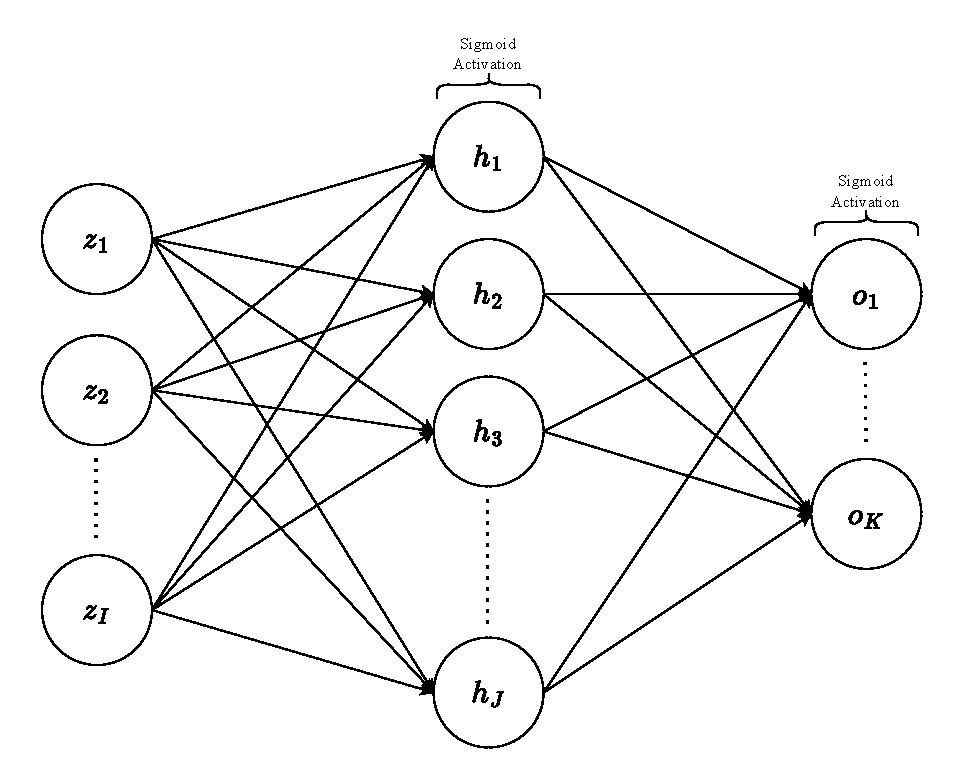
\includegraphics[width=0.45\textwidth]{images/NNarch.pdf}
	\caption{Neural network architecture. Here, $z_i$ represents input units, $h_i$ represents hidden units, and $o_i$ represents output units.}
	\label{fig:nnarch}
\end{figure}

The grid search is only performed once using the MSE Loss given in Equation~\ref{eq:mse} in the passive learning setting. Here, $N$ represents the number of training patterns, $K$ represents the number of output units, $t_k^{(i)}$ is the target value for output unit $k$ in pattern $i$, $o_k^{(i)}$ is the network output of unit $k$ in pattern $i$, $w_j$ is the weight parameter and $\lambda$ is the weight decay coefficient. The same parameter values obtained from the passive learning grid search are used in the active learning procedures in order to maintain the focus of the comparison on the algorithms and not the parameters. SGD is used to determine the optimal parameter values.
\begin{equation}
L_{\text{MSE+WD}} = \frac{1}{N} \sum_{i=1}^{N} \sum_{k=1}^{K} \big( t_{k}^{(i)} - o_{k}^{(i)} \big)^2
+\lambda \sum_{j} w_j^2
\label{eq:mse}
\end{equation}


\subsection{Output Sensitivity Algorithm}
% - Detailed implementation of output sensitivity analysis
% - Detailed implementation of uncertainty sampling
% - Query selection mechanisms
% - Batch size considerations for active learning
The output sensitivity active learning implementation follows the background derivations previously described. A conservative pattern selection constant, $\beta = 0.9$ is used. That is, the algorithm only picks the most informative samples, keeping the training subset small at first. 

The algorithm operates by repeatedly training the neural network on training subset $D_T$ until a termination criterion on $D_T$ is triggered. In this implementation, a budget of 1000 epochs is used. The exact gradient-based output sensitivity is computed using Equation~\ref{eq:sens_mat}. The pattern informativeness is then computed using both sum-norm and max-norm metrics in Equation~\ref{eq:inform} and \ref{eq:mn}. The average pattern informativeness is calculated and multiplied by $(1 - \beta)$ to determine the selection threshold. The patterns with informativeness above this threshold are selected from the candidate set. A safety mechanism was implemented here to ensure that at least one sample per class is kept. Initially these calculations were performed linearly, however vectorising them results in a massive improvement in performance. A selection interval parameter is used to determine after how many epochs the selection takes place, this is set to one unless otherwise stated.

\subsection{Uncertainty Sampling Algorithm}
Both entropy and ensemble-based uncertainty sampling were implemented. The Pool-Based Active Learning Framework described in Algorithm~\ref{alg:pool_active_learning} is implemented. First, the algorithm starts with a small labelled set $L$ and large unlabelled pool $U$. The initial labelled set is defined as the smaller of 10\% of the training data or 10 observations. Then, for each query iteration, compute the utility (uncertainty) for all the samples in $U$. This is computed using the softmax of the output units,to obtain probabilities for use in the equation Equation~\ref{eq:entropy}. Further normalise the raw entropy obtained from Equation~\ref{eq:entropy} by dividing by $\log(C)$, this is to ensure that the entropy is in the range [0, 1]. The highest utility sample is selected and its label queried, then moved from $U$ to $L$. Now, simply retrain the model on the updated $L$ set and repeat this process until the budget is exhausted. Here, the budget is defined as the number of remaining samples.

For the ensemble-based approach, three independent neural networks are trained simultaneously with different random weight initialisations to create diversity in their learned representations. Rather than using entropy of a single model's output distribution as the uncertainty metric, the disagreement among ensemble members is exploited. Specifically, for each unlabelled sample $\mathbf{x}_i \in U$, perform forward passes through all ensemble members to obtain softmax-normalised probability distributions $\{\mathbf{p}^{(1)}_i, \mathbf{p}^{(2)}_i, ..., \mathbf{p}^{(n_{ensemble})}_i\}$. The uncertainty is then quantified as the total predictive variance across the ensemble using Equation~\ref{eq:var-e}. Higher variance indicates greater disagreement among models, suggesting the sample lies in an ambiguous region of the feature space where additional labelled data would be most informative. During training, all ensemble members are updated synchronously on the same labelled set $L$ using independent optimisers, and final predictions are made via majority voting across the ensemble. This approach trades increased computational cost (linear in $n_{ensemble}$) for potentially better-calibrated uncertainty estimates, particularly valuable when dealing with limited labelled data where single-model confidence may be poorly calibrated.

\subsection{Software and Hardware Specifications}
% - Programming language and libraries used
% - Computational resources
% - Code repository reference (as required)
All experiments were performed on a Fedora Linux system with a 13th Gen Intel Core i3-13100 x8 CPU and 16GiB of memory. The code for this paper is available on GitHub \cite{github}.



\section{Empirical Process}
The datasets along with their respective pre-processing measures are presented in this section, followed by a summary of the performance criteria and the experimental design. Finally, the statistical analysis framework is described.
\subsection{Dataset Selection and Pre-processing}
% - Description of at least 3 classification problems
% - Description of at least 3 function approximation problems  
% - Varying complexity justification
% - Data preprocessing steps with motivations
% - Train/validation/test splits
Three classification and regression problems were selected. One simple, one medium, and one hard problem were selected for each to illustrate how the algorithms apply to varying problem complexities. 

The iris dataset was used as the simplest classification problem with four predictors and three target classes. The distribution of the classes is noted in Table~\ref{tab:dataset_descriptions}. The wine cultivar dataset was used as a dataset of medium complexity. It contains 13 feature variables and a target variable of three classes representing different wine cultivars. The fashion-MNIST dataset is a more complex dataset containing pixel information from $28 \times 28$ grey scale images. There are 10 equally distributed target classes each representing different articles of clothing. 

An artificial function approximation task was created using
\[
y = \sin(2 \pi x) + \text{noise}
\]
where the noise is Gaussian noise centred at 0 with a standard deviation of 0.1. The California housing dataset is a medium complexity function approximation problem with nine features and the target variable is the median house value. The energy efficiency dataset is the final function approximation task considered with eight features used to predict the heating load of a building.

\begin{table}[htbp]
	\caption{Dataset Descriptions}
	\label{tab:dataset_descriptions}
	\centering
	\begin{tabular}{|l|l|l|}
		\hline
		\textbf{Dataset} & \textbf{Distribution / Notes} & \textbf{Source} \\
		\hline
		Iris & \begin{tabular}[c]{@{}l@{}}setosa -- 33.3\% \\ versicolor -- 33.3\% \\ virginica -- 33.3\%\end{tabular} & \cite{iris} \\
		\hline
		Wine & \begin{tabular}[c]{@{}l@{}}cultivar 0 -- 33.1\% \\ cultivar 1 -- 39.9\% \\ cultivar 2 -- 27.0\%\end{tabular} & \cite{wine} \\
		\hline
		Fashion-MNIST & 10 equally distributed classes & \cite{mnist} \\
		\hline
		Sine + Noise & sine function + Gaussian noise & synthetic \\
		\hline
		California Housing & - & \cite{housing} \\
		\hline
		Energy Efficiency & - & \cite{energy} \\
		\hline
	\end{tabular}
\end{table}



% describe on a per issue basis which datasets had it and what was done and why IMPORTANT WHY
% missing values
Only the California housing dataset contained 207 missing values in the \texttt{total\_bedrooms} column. These missing values were imputed with the median for a safe estimate that is less sensitive to outliers. None of the other datasets contained missing values.

% ID column: Iris,
The iris dataset contained an ID feature which was dropped since it provides no predictive power to the model.

% scale [-1, 1]: all
All the features were scaled to the range $[-1, 1]$ since the hidden layer uses the sigmoid activation function. If unscaled inputs were fed into the model, the linear outputs could be very large for positive or negative numbers. This would saturate the sigmoid function leading to vanishing gradients. The function approximation tasks' target variables were scaled to bring the values into a range consistent with the network's activations and makes optimisation much more stable. Obviously, at prediction time, the scaling is inverted.

% one hot encode: Iris target, wine target, fashion target, Housing one feature var
For the iris, wine, and fashion-MNIST datasets the target variables were one-hot encoded so the neural network can provide a probability distribution across classes. The housing dataset had one categorical feature, \texttt{ocean\_proximity}, which was one-hot encoded so that the neural network could interpret the feature levels without assuming an ordinal relationship.

In order for the frameworks to be applied to the various problems, the variables that were changed were: the input and output dimensions of the neural network, number of epochs, and for regression the output activation function was removed. The size of the datasets and number of epochs are presented in Table~\ref{tab:dataset_epochs}. A test train split of 20/80 was considered for all approaches and datasets.

\begin{table}[htbp]
	\centering
	\caption{Dataset sizes and number of epochs used for training}
	\begin{tabular}{|l|c|c|}
		\hline
		\textbf{Dataset} & \textbf{Size} & \textbf{Epochs} \\
		\hline
		Iris & 150 & 1000 \\
		Wine & 178 & 2000 \\
		Fashion-MNIST & 70,000 & 1000 \\
		\hline
		Sine + Noise & 500 & 1000 \\
		Housing & 20,640 & 200 \\
		Energy & 768 & 200 \\
		\hline
	\end{tabular}
	\label{tab:dataset_epochs}
\end{table}



\subsection{Performance Criteria}
% - Classification metrics: accuracy, precision, recall, F1-score
% - Function approximation metrics: MSE, MAE, R²
% - Learning curve analysis
% - Sample efficiency measures
% - Statistical significance testing approach
For the classification tasks, accuracy was the primary metric used for model performance evaluation across all learning strategies. The F1-Score was also recorded and considered for a more comprehensive, balanced metric. The precision and recall were also tracked. In each training iteration, the number of training observations seen by the model are recorded as it trains. The training set size reduction for the active learning methods was recorded across the epochs. Epochs to convergence was recorded for each method, that is, the number of training epochs required for the model to achieve a stable performance. The convergence rate was computed by calculating the proportion of the trials achieving the convergence threshold.

For the function approximation tasks, Mean Squared Error (MSE) served as the primary performance metric, directly measuring the average squared deviation between predicted and actual target values. Similar to classification tasks, the number of training observations presented to the model was tracked throughout training to assess sample efficiency. Training and validation losses were monitored across epochs to evaluate convergence behaviour and detect potential overfitting or underfitting patterns.


\subsection{Experimental Design}
% - Cross-validation strategy
% - Multiple runs for statistical reliability
% - Control parameter optimization process
% - Hyperparameter tuning methodology
% - Fair comparison ensuring protocols
Due to the stochastic nature of the weight initialisation process, 50 trial runs were performed for each method for statistical reliability. Each run included five-fold stratified cross-validation. That is, the distribution of the target classes in the original data is maintained in the training and validation sets. In order to optimise the control parameters, a grid search was performed. First, the hidden layer size was varied across $\{64, 128, 256, 512\}$, allowing the model capacity to range from relatively compact (64 units) to more expressive (512 units). The learning rate was chosen from  $\{0.01, 0.05, 0.1, 0.5\}$, where smaller values yield slower but stable convergence, and larger values speed up training at the risk of overshooting minima. To control overfitting, the following weight decay values $\{0.0, 0.001, 0.01, 0.1\}$ were considered, where higher values apply stronger $L_2$ regularisation on the weights. Finally, momentum was introduced with values $\{0.0, 0.5, 0.9, 0.95\}$, ranging from standard stochastic gradient descent (no momentum) to strongly accelerated updates (high momentum). Since each parameter is considered independently, the total number of grid search configurations is the Cartesian product of these sets, i.e., $4 \times 4 \times 4 \times 4 = 256$ distinct control parameter combinations. The grid search was performed on the passive learning model setup, and the parameters obtained were then applied to the active learning approaches since the primary focus of this study is to compare the active learning techniques, and not the control parameters.

\subsection{Statistical Analysis Framework}
% - Hypothesis testing approach
% - Significance levels
% - Multiple comparison corrections
% - Effect size measurements
To ensure a rigorous comparison of the learning approaches, a comprehensive statistical framework was implemented across multiple levels of analysis.
\subsubsection{Normality Assessment}
Normality was first assessed to determine whether the model results come from a normal distribution. That is, the Shapiro-Wilk test provided insight as to consult parametric or non-parametric tests. Some of the further statistical tests considered have a normality assumption, and therefore cannot be considered for non-normal results.

\subsubsection{Omnibus Testing}
The Friedman test \cite{friedman1937} is the non-parametric equivalent of repeated measures ANOVA and has the null hypothesis that all the methods performed identically.  The test ranked methods within each trial and then compared the average rank with a significance level of $\alpha=0.05$. If $p <0.05$, the analysis proceeded to post-hoc pairwise tests, if $p \ge 0.05$, no significant differences existed.

\subsubsection{Pairwise Comparisons}
The Wilcoxon signed-rank test was applied as a non-parametric paired comparison test. Since four methods were compared, this resulted in $\binom{4}{2} = 6$ pairwise comparisons. To control for Type I error inflation due to multiple comparisons, the Bonferroni correction was applied \cite{bonferroni1936}, adjusting the significance threshold to $\alpha_{adjusted} = 0.05 / 6 \approx 0.0083$. Without this correction, the probability of at least one false positive across all comparisons would be approximately $1 - 0.95^6 \approx 0.26$. Methods were considered significantly different only if $p < \alpha_{adjusted}$.

\subsubsection{Critical Difference Analysis}
Critical difference plots were created to provide a visual representation of all the pairwise comparison tests simultaneously. The methods are ranked from one to four within each trial and averaged over all 50 trials. Methods with a lower average rank are said to have better performance. The critical difference (CD) was calculated using the Nemenyi post-hoc test \cite{nemenyi1963} as $\text{CD} = q_{\alpha} \sqrt{k(k+1)/(6N)}$, where $k=4$ methods, $N=50$ trials, and $q_{\alpha}$ is the critical value from the Studentized range distribution at $\alpha = 0.05$. Methods differing by more than CD in average rank are considered significantly different, with connected horizontal bars indicating non-significant differences.


\subsubsection{Significance Levels and Multiple Testing}
All hypothesis tests employed a significance level of $\alpha = 0.05$. The family-wise error rate across the six pairwise comparisons was controlled through Bonferroni correction, ensuring the overall Type I error probability remained at 0.05. This conservative approach reduces the risk of false positive findings when conducting multiple statistical tests on the same dataset.



\section{Results \& Discussion}
% (50 marks - largest section, most critical)
The metrics obtained from the various approaches on the six datasets are presented in this section. The performance of the passive and active learning approaches are also compared by explaining the accuracies and training statistics. 


\subsection{Control Parameter Optimisation Results}
% - Optimal hidden unit numbers for each problem
% - Optimal penalty coefficients
% - Control parameter values with justifications
% - Convergence analysis
The grid search obtained a variety of results as exhibited in Table~\ref{tab:datasets}. Surprisingly, the weight decay parameter was only used in two of the datasets. The momentum values remained quite similar at around 0.9 whilst most of the learning rate parameters also remained at 0.5 except for the wine dataset. The number of hidden units was often small due to the power of neural networks being able to approximate functions even with a smaller number of hidden units, especially when the functions were less complex.

\begin{table}[htbp]
	\centering
	\caption{Parameters obtained from grid search}
	\begin{tabular}{|l|c|c|c|c|}
		\hline
		\textbf{Dataset} & \makecell{\textbf{Hidden} \\ \textbf{Units}} & \makecell{\textbf{Weight} \\ \textbf{Decay}} & \makecell{\textbf{Learning} \\ \textbf{Rate}} & \textbf{Momentum} \\
		\hline
		Iris & 512 & 0.1 & 0.5 & 0.9 \\
		Wine & 64 & 0 & 0.01 & 0.9 \\
		Fashion-MNIST & 512 & 0 & 0.5 & 0.95 \\
		\hline
		Sine + Noise & 64 & 0.1 & 0.5 & 0.95 \\
		Housing & 64 & 0 & 0.5 & 0.95 \\
		Energy & 64 & 0 & 0.5 & 0.9 \\
		\hline
	\end{tabular}
	\label{tab:datasets}
\end{table}







\subsection{Classification Problem Results}
% - Performance comparison across all three approaches
% - Learning curves showing sample efficiency
% - Statistical significance of differences
% - Problem-specific performance analysis
% - Tables and figures with proper captions

% speaking about the table
For the simple iris dataset, all the methods performed similarly, as shown in Table~\ref{tab:comparison}. All the approaches maintained a stable performance with the standard deviations remaining low. Slightly more drop off in performance is seen as the complexity of the dataset was increased. That is, for the fashion-MNIST dataset the entropy and the ensemble uncertainty active learning approaches had a small, but noticeable, decrease in performance compared to the passive learning approach.

% loss curves
Figure~\ref{fig:iris-los} indicates that both the passive learning and SASLA approaches were stable during training and not exhibiting any noticeable overfitting behaviour. The entropy and ensemble uncertainty sampling approaches were slightly less stable, but still converged well after the full 1000 epochs had been performed. This is understandable, since the training sets start off small and therefore more variability can be expected. Similar trends are observed in Figure~\ref{fig:wine-loss}, however, with slightly less variability for the uncertainty sampling approaches. For the fashion-MNIST dataset in Figure~\ref{fig:fashion-loss}, the validation losses appear to land higher than the training losses after the 1000 epochs. This gap suggests that the models may be under-regularised or struggling to generalise fully to the more complex and diverse patterns in the fashion-MNIST dataset.

% generalisation factors
The strength of the entropy uncertainty sampling can be seen in Figure~\ref{fig:gf_iris}, where the generalisation factor exceeds that of the passive learning approach at roughly 2000 epochs. This indicates that this uncertainty sampling approach was efficient at selecting useful samples for training at early stages. This highlights the advantage of active learning, as it is able to prioritise informative samples that accelerate model improvement compared to random selection. However, this is not the case for all datasets, as Figure~\ref{fig:gf_wine} and Figure~\ref{fig:gf_fashion} show that for bigger datasets, considering all samples is more effective at achieving a better overall performance. 

% f1 scores
Again in Figure~\ref{fig:f1_iris}, the entropy uncertainty sampling performs well at a low number of epochs. Figure~\ref{fig:f1_wine} shows that the entropy uncertainty sampling found some super informative observations early on which lead to it improving performance, however as it added more less informative observations, the F1-score then decreased again to align with the other approaches. The SASLA approach can get led in the wrong direction and the performance can decrease, this is seen in Figure~\ref{fig:f1_fashion} where the F1-score decreases noticeably after 500 epochs.




\subsection{Function Approximation Results}
% - Detailed results for each regression problem
% - Comparison of convergence rates
% - Sample efficiency analysis
% - Performance variance across runs

% table
For function approximation tasks, the SASLA and entropy uncertainty sampling approaches performed worse when applied to smaller datasets, specifically the synthetic dataset in Table~\ref{tab:comparison_reg}. The passive approach achieved the lowest error, while SASLA and entropy both introduced a noticeable increase in MSE, with entropy uncertainty in particular exhibiting a very high variance across runs. Ensemble uncertainty fell in between, outperforming SASLA and entropy but still lagging behind passive learning.

For the housing dataset, the performance of all methods converged, with only minor differences in MSE and relatively low variance across runs. This suggests that for a moderately sized real-world dataset, the choice of active learning strategy had limited impact compared to passive sampling.

In contrast, for the energy dataset, clear divergence emerged between the strategies. While SASLA and passive approaches remained close in performance, entropy uncertainty once again performed poorly, showing both high error and instability. Ensemble uncertainty also underperformed relative to passive learning, but achieved significantly better results than entropy-based sampling.

% loss curves
In general, few epochs were required for the regression tasks to converge clearly. Figure~\ref{fig:losses_synfunc} shows that all the methods converged in about 200 epochs. The trend is seen more closely in Figure~\ref{fig:losses_housing}, where the entropy and ensemble uncertainty approaches took about double the number of epochs to converge compared to the passive and SASLA approaches. That is, they converged after about 100 epochs compared to 50 for the other two approaches. The SASLA approach varied significantly during early stages of training in Figure~\ref{fig:losses_energy}. This instability in SASLA’s early training phase likely stems from its reliance on the adaptive sampling, which can introduce high variance in gradient updates before the model has established a stable representation.

% gen factor
The uncertainty approaches showed their true power in Figure~\ref{fig:gf_housing} where we see they achieved an impressive generalisation factor early in training when only a few patterns had been presented to them. The passive and SASLA approaches more observations to achieve a similar performance. This is expected, as the models were able to find informative samples early on through the active sampling process.

\subsection{Comparative Analysis}
% - Overall ranking of approaches
% - Problem-dependent performance patterns
% - Sample efficiency comparison
% - Computational cost analysis
% - Advantages and disadvantages of each approach

% Computation time
Computational efficiency varied considerably across methods and datasets, as shown in Table~\ref{tab:computation_times}. Ensemble uncertainty consistently required the longest training times due to maintaining multiple models, particularly evident in the housing dataset (12.64s vs 0.60s for passive). SASLA incurred moderate overhead from sensitivity calculations, approximately 1.5× slower than passive learning on average. Entropy uncertainty sampling showed mixed results, where it was faster than passive on some datasets (synthetic: 0.95s vs 0.97s) but substantially slower on others (housing: 2.43s vs 0.60s), likely due to the cost of computing entropy over large unlabelled pools. For smaller datasets like iris and wine, the computational overhead of active learning was minimal in absolute terms, though proportionally significant. These results suggest that while active learning methods can reduce sample complexity, practitioners must weigh potential gains in sample efficiency against increased computational costs, particularly when using ensemble-based approaches or processing large unlabelled pools.

% statistical comparison
For small datasets, the models had equivalent performance, based on the critical difference plot in Figure~\ref{fig:cd_iris} for the iris dataset. The critical difference plot shows that while ensemble uncertainty achieved the best average rank (2.39) and uncertainty sampling the worst (2.64), all four methods are connected by horizontal lines indicating no statistically significant differences between them at the 0.05 level. This means that despite numerical differences in rankings, all methods perform equivalently from a statistical perspective. 

In contrast, the plot for the fashion-MNIST dataset in Figure~\ref{fig:cd_fashion} shows the simpler approaches (passive learning and SASLA) significantly outperform the more complex active learning methods (entropy uncertainty sampling and ensemble uncertainty), with ensemble uncertainty performing worst overall. Here, the passive learning and SASLA approaches are not significantly different from each other, since the difference of 0.09 is less than the critical difference of 0.663. The SASLA and passive learning approaches exhibited similar behaviour in the energy efficiency dataset seen in Figure~\ref{fig:cd_energy}. 

For the synthetic dataset, the passive learning showed to be different from the active learning approaches. This is observed in Figure~\ref{fig:cd_synfunc}.

Table~\ref{tab:omnibus} confirms significant differences exist among the compared methods across all four datasets (fashion, synthetic, housing, and energy). Both parametric tests (ANOVA F, Friedman $\chi^2$) and non-parametric tests (Kruskal-Wallis H) consistently yield p-values below 0.001, which is well below the $\alpha = 0.05$ significance threshold. These results justify proceeding with post-hoc pairwise comparisons (like the critical difference plots) to identify which specific methods differ from each other, as the omnibus tests confirm that not all methods perform equally.

\begin{table}[htbp]
	\caption{Omnibus Test Results}
	\label{tab:omnibus}
	\centering
	\small
	\begin{tabular}{lccc}
		\hline
		\textbf{Dataset} & \textbf{Test} & \textbf{Statistic} & \textbf{p-value} \\
		\hline
		Fashion   & Friedman $\chi^2$     & 125.80 & $<0.001$ \\
		& ANOVA F               & 27.87  & $<0.001$ \\
		\hline
		Synthetic & Friedman $\chi^2$     & 62.38  & $<0.001$ \\
		& Kruskal-Wallis H      & --     & $<0.001$ \\
		\hline
		Housing   & Friedman $\chi^2$     & 85.75  & $<0.001$ \\
		& Kruskal-Wallis H      & 104.07 & $<0.001$ \\
		\hline
		Energy    & Friedman $\chi^2$     & 110.33 & $<0.001$ \\
		& Kruskal-Wallis H      & 140.71 & $<0.001$ \\
		\hline
	\end{tabular}
	\begin{flushleft}
		\footnotesize All tests indicate significant differences among methods at $\alpha = 0.05$.
	\end{flushleft}
\end{table}


\section{Conclusions}
Active learning approaches did not consistently outperform traditional passive learning with regards to key metrics. These approaches did however show efficient training characteristics. Training samples are selected in a more informed fashion which provides benefits during training. Passive learning remains competitive and simpler to implement for most scenarios. SASLA proved somewhat of a middle ground with moderate overhead required. Ensemble uncertainty incurs significant computational costs which struggle to outweigh training benefits. 

A single hidden-layer architecture may not accurately reflect more complex deep learning approaches and a fixed selection parameter of 0.9 may not be optimal for all problems. Future work could include considering adaptive selection thresholds and extension into deep neural network architectures.

Active learning is not a universal solution and the overheads should be carefully considered before electing an active learning strategy over traditional passive learning.

\bibliographystyle{IEEEtran}
\bibliography{references}

\appendices
\section{Additional Results}

\begin{table*}[ht]
	\caption{Comparison of classification accuracies $\pm$ standard deviation }
	\label{tab:comparison}
	\centering
	\begin{tabular}{|l|c|c|c|c|}
		\hline
		\textbf{Dataset} & \textbf{Passive} & \textbf{SASLA} & \textbf{Entropy Uncertainty} & \textbf{Ensemble Uncertainty} \\
		\hline
		Iris Train & $0.9819 \pm 0.0066$& $0.9803 \pm 0.0073$ & $0.9692\pm 0.0105$& $0.9780 \pm 0.0084$ \\
		Iris Test & $0.9819 \pm 0.0292$ & $0.9653 \pm 0.0298$  & $0.9613 \pm 0.0322$ & $0.9660 \pm 0.0302$  \\
		\hline
		Wine Train& $0.9834 \pm 0.0050$ & $0.9834 \pm 0.0047$ & $0.9799 \pm 0.0059$ & $0.9693 \pm 0.0114$ \\
		Wine Test & $0.9750 \pm 0.0237$ & $0.9728 \pm 0.0238$  & $0.9722 \pm 0.0255$ & $0.9506 \pm 0.0339$ \\
		\hline
		Fashion-MNIST Train & $0.9030 \pm 0.0023$ & $0.9033 \pm 0.0027$ & $0.8688 \pm 0.0034$ & $0.8513 \pm 0.0029$ \\
		Fashion-MNIST Test & $0.8414 \pm 0.0109$  & $0.8409 \pm 0.0113$  & $0.8309 \pm 0.0110$ & $0.8246 \pm 0.0100$  \\
		\hline
	\end{tabular}
\end{table*}

\begin{table*}[ht]
	\caption{Comparison of regression MSE $\pm$ standard deviation }
	\label{tab:comparison_reg}
	\centering
	\begin{tabular}{|l|c|c|c|c|}
		\hline
		\textbf{Dataset} & \textbf{Passive} & \textbf{SASLA} & \textbf{Entropy Uncertainty} & \textbf{Ensemble Uncertainty} \\
		\hline
		Synthetic Train & $0.0301 \pm 0.0550$& $0.1148 \pm 0.0770$ & $0.1402 \pm 0.3900$& $0.0752 \pm 0.0877$ \\
		Synthetic Test & $0.0321 \pm 0.0609$ & $0.1146 \pm 0.0758$  & $0.1389\pm 0.3713$ & $0.0746 \pm 0.0872$   \\
		\hline
		Housing Train& $0.0835 \pm 0.0202$ & $0.0921 \pm 0.0080$ & $0.1022 \pm 0.0194$ & $0.1023 \pm 0.0179$ \\
		Housing Test & $0.0842 \pm 0.0217$ & $0.0926 \pm 0.0088$  & $0.1027 \pm 0.0198$ & $0.1027 \pm 0.0188$ \\
		\hline
		Energy Train & $0.0442 \pm 0.0267$ & $0.0455 \pm 0.0320$ & $0.2522 \pm 0.2416$ & $0.1232 \pm 0.0411$ \\
		Energy Test & $0.0349 \pm 0.0258$  & $0.0459 \pm 0.0315$  & $0.2519 \pm 0.2431$ & $0.1210 \pm 0.0409$  \\
		\hline
	\end{tabular}
\end{table*}

%\begin{table*}[ht]
%	\caption{Comparison of number of pattern presentations $\pm$ standard deviation}
%	\label{tab:comparison_patterns}
%	\centering
%	\begin{tabular}{|l|c|c|c|c|}
%		\hline
%		\textbf{Dataset} & \textbf{Passive} & \textbf{SASLA} & \textbf{Entropy Uncertainty} & \textbf{Ensemble Uncertainty} \\
%		\hline
%		Iris & $760.8 \pm 728.99$ & $1046.4 \pm 693.53$ & $801.6 \pm 668.75$ & $1485.6 \pm 711.10$ \\
%		\hline
%		Synthetic & $60112 \pm 10025.90$ & $55256 \pm 10809.48$ & $76520 \pm 19876.14$ & $84704 \pm 12638.88$ \\
%		\hline
%		Housing & $1246656 \pm 278915.98$ & $1164426.24 \pm 197295.67$ & $2105280 \pm 570553.52$ & $2256860.16 \pm 417063.70$ \\
%		\hline
%	\end{tabular}
%\end{table*}

\begin{table*}[ht]
	\caption{Computation time (in seconds) $\pm$ standard deviation for different methods}
	\label{tab:computation_times}
	\centering
	\begin{tabular}{|l|c|c|c|c|}
		\hline
		\textbf{Dataset} & \textbf{Passive} & \textbf{SASLA} & \textbf{Entropy Uncertainty} & \textbf{Ensemble Uncertainty} \\
		\hline
		Iris & $4.664 \pm 0.185$ & $6.731 \pm 0.337$ & $5.512 \pm 0.158$ & $1.630 \pm 0.047$ \\
		\hline
		Wine & $9.754 \pm 0.745$ & $12.991 \pm 0.454$ & $9.860 \pm 0.234$ & $3.565 \pm 0.263$ \\
		\hline
		Fashion & $8.757 \pm 0.291$ & $21.378 \pm 0.815$ & $12.397 \pm 0.768$ & $23.825 \pm 0.705$ \\
		\hline
		Synthetic Functions & $0.968 \pm 0.046$ & $1.094 \pm 0.064$ & $0.950 \pm 0.041$ & $2.251 \pm 0.101$ \\
		\hline
		Housing & $0.596 \pm 0.051$ & $0.491 \pm 0.107$ & $2.431 \pm 0.079$ & $12.642 \pm 0.577$ \\
		\hline
		Energy & $1.376 \pm 0.149$ & $1.444 \pm 0.084$ & $1.438 \pm 0.054$ & $4.501 \pm 0.134$ \\
		\hline
	\end{tabular}
\end{table*}


\begin{figure}[!t]
	\centering
	\caption{Losses for training of frameworks with the iris dataset.}
	\label{fig:iris-los}
	
	\begin{subfigure}{\linewidth}
		\centering
		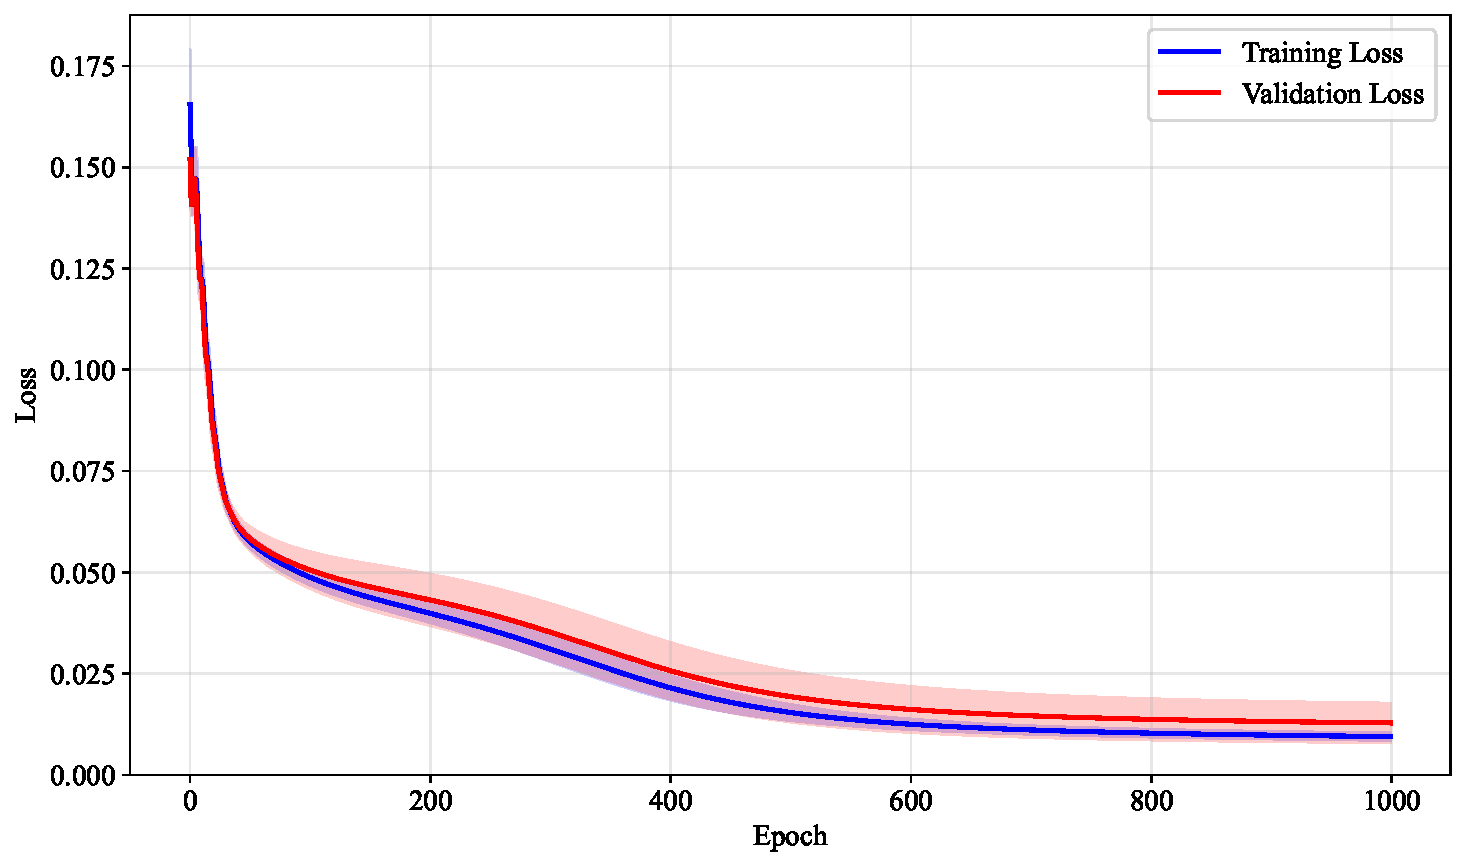
\includegraphics[width=\linewidth]{../results/iris/losses.pdf}
		\caption{Passive learning losses.}
		\label{fig:losses}
	\end{subfigure}
	
	\vspace{0.1em}
	
	\begin{subfigure}{\linewidth}
		\centering
		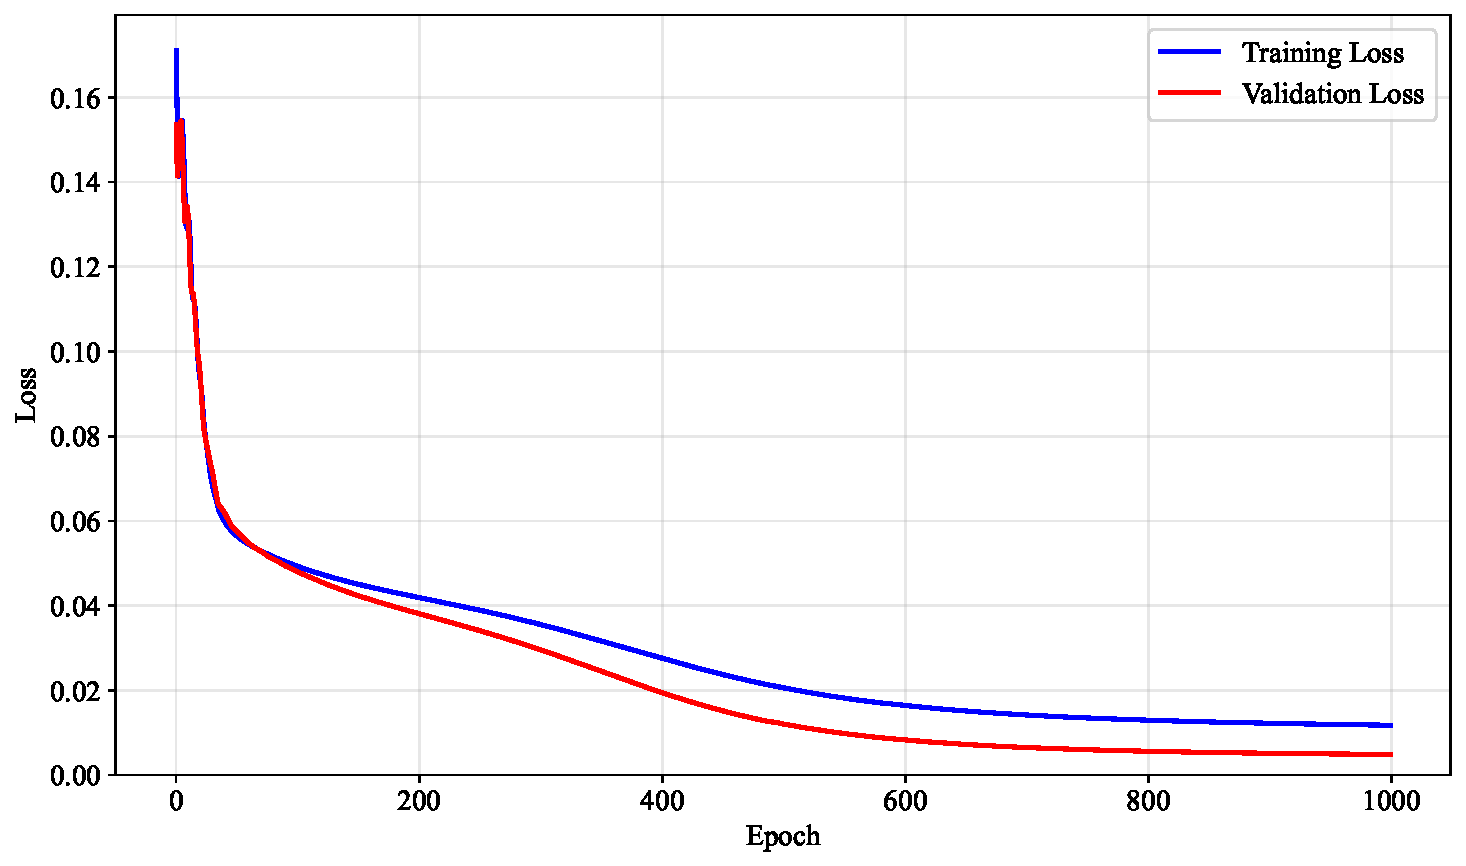
\includegraphics[width=\linewidth]{../results/iris/os_losses.pdf}
		\caption{SASLA losses.}
		\label{fig:os_losses}
	\end{subfigure}
	
	\vspace{0.1em}
	
	\begin{subfigure}{\linewidth}
		\centering
		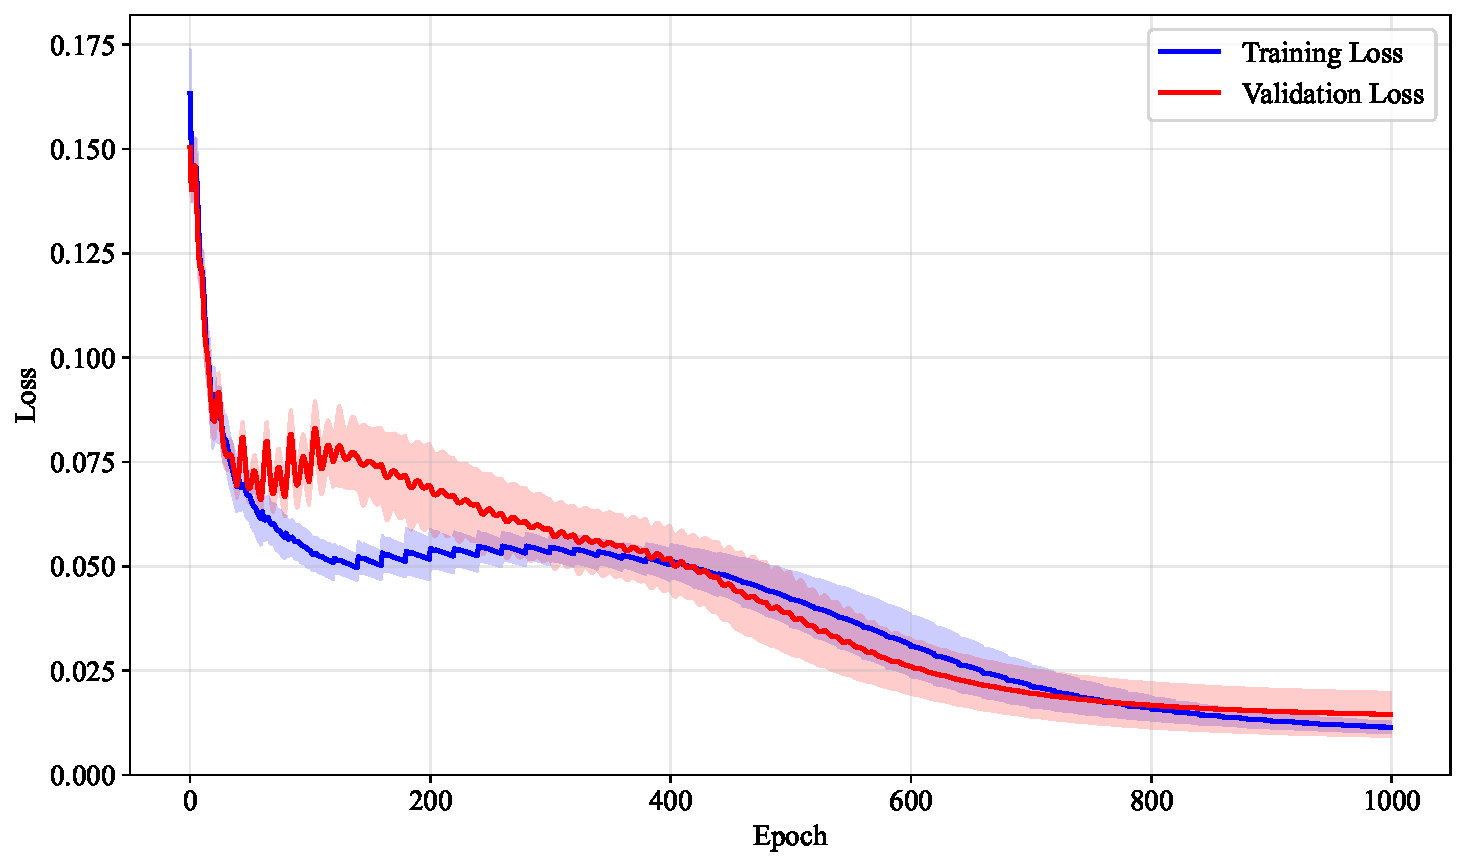
\includegraphics[width=\linewidth]{../results/iris/us_losses.pdf}
		\caption{Entropy uncertainty sampling losses.}
		\label{fig:us_losses}
	\end{subfigure}
	
	\vspace{0.1em}
	
	\begin{subfigure}{\linewidth}
		\centering
		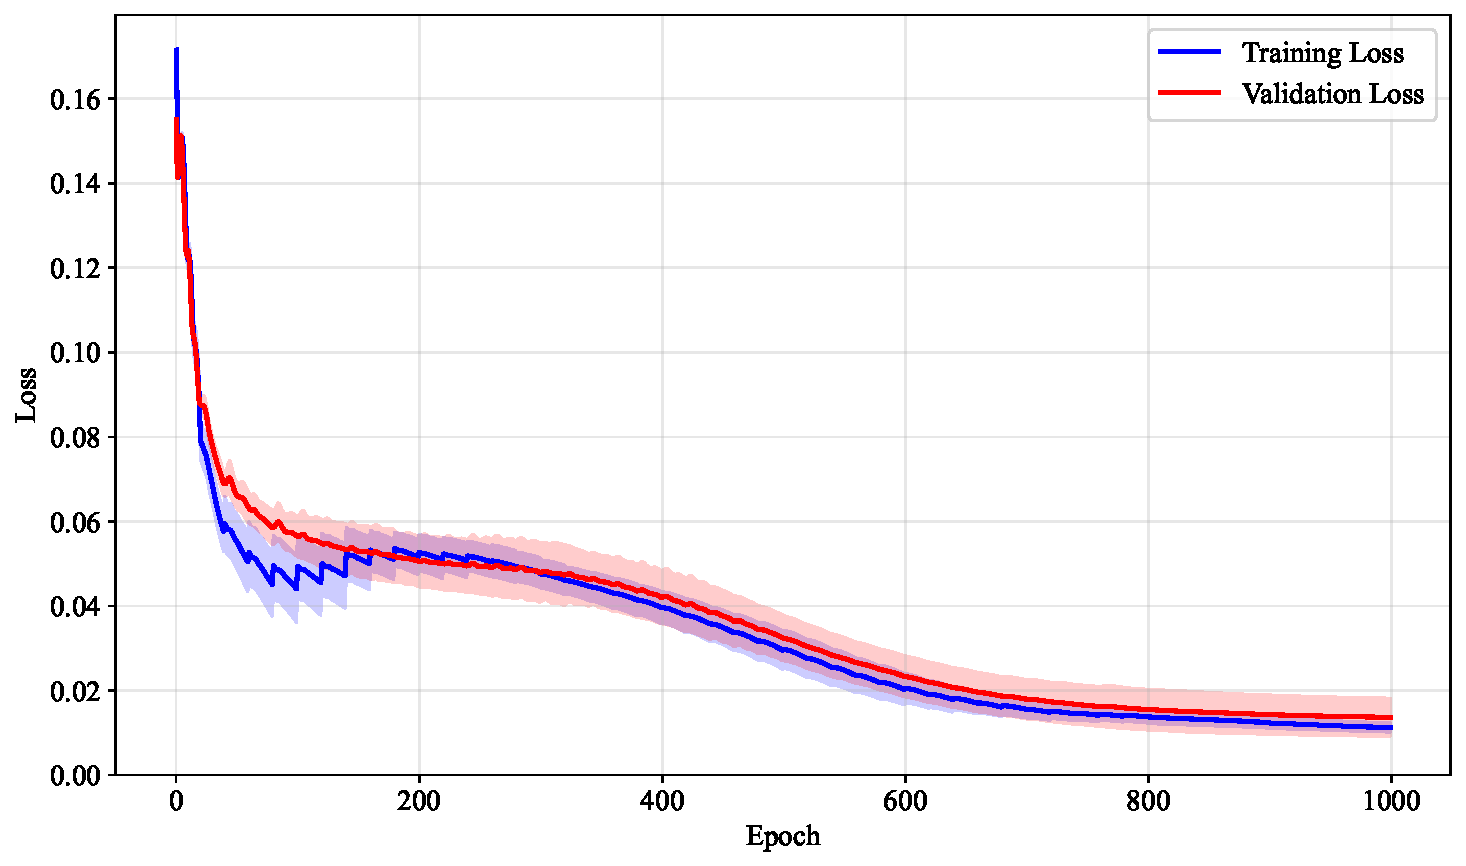
\includegraphics[width=\linewidth]{../results/iris/ensemble_us_losses.pdf}
		\caption{Ensemble uncertainty sampling losses.}
		\label{fig:ensemble_us_losses}
	\end{subfigure}
\end{figure}

\begin{figure}[!t]
	\centering
	\caption{Losses for training of frameworks with the wine dataset.}
	\label{fig:wine-loss}
	\begin{subfigure}{\linewidth}
		\centering
		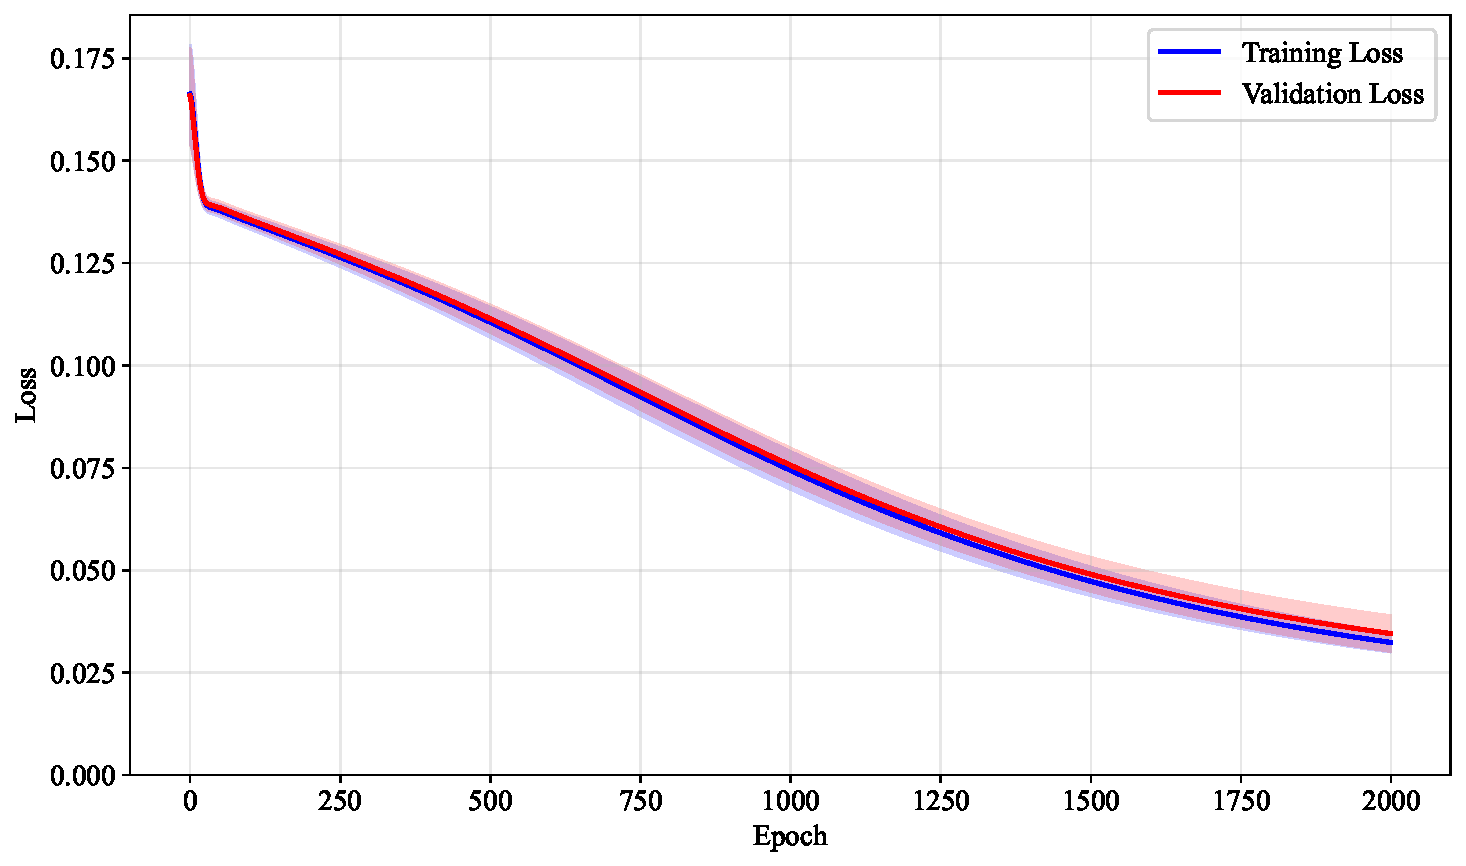
\includegraphics[width=\linewidth]{../results/wine/losses.pdf}
		\caption{Passive learning losses.}
		\label{fig:losses_wine}
	\end{subfigure}
	
	\vspace{0.1em}
	
	\begin{subfigure}{\linewidth}
		\centering
		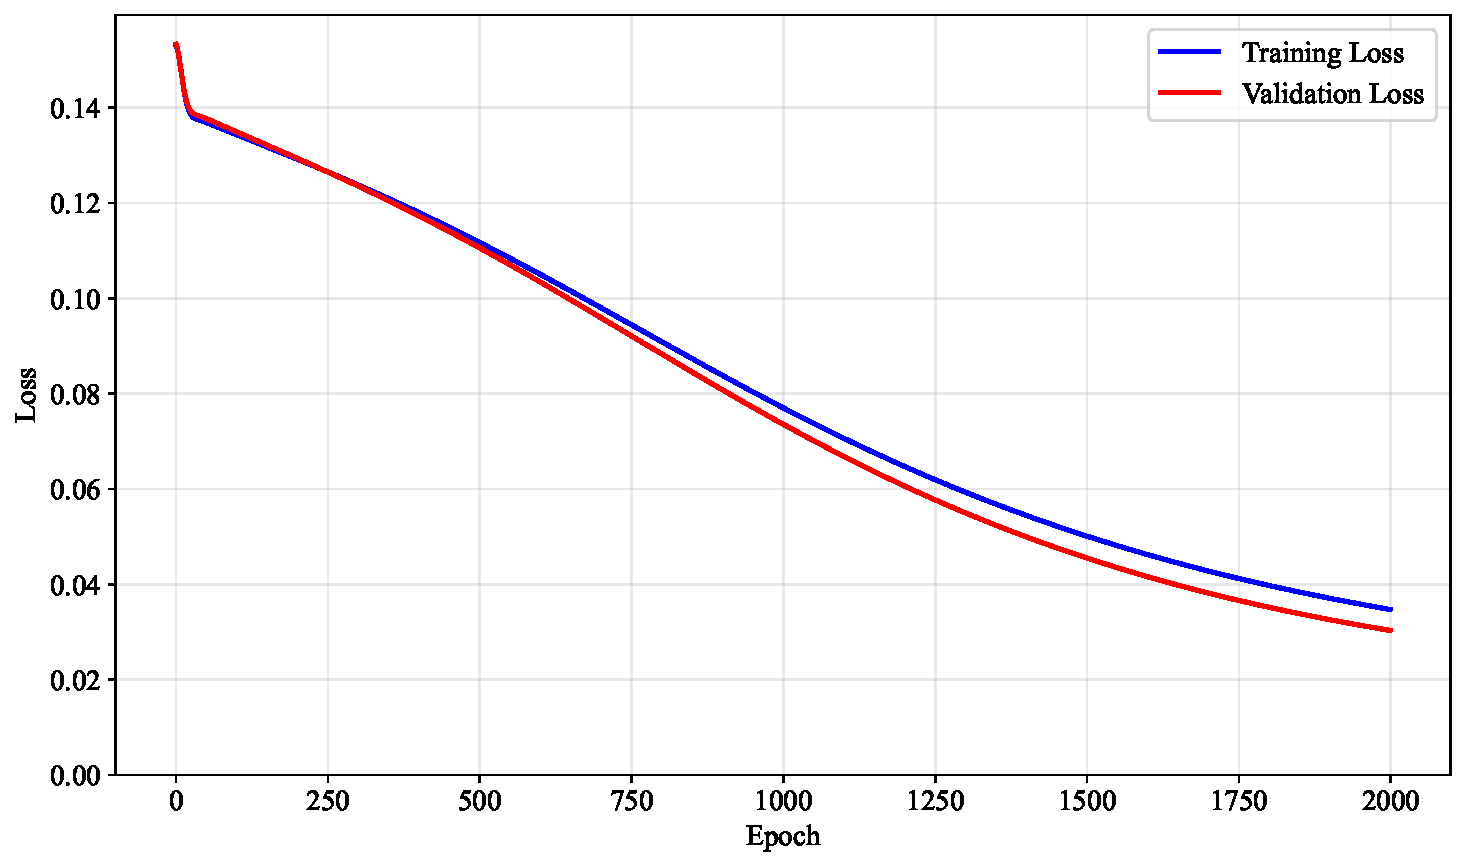
\includegraphics[width=\linewidth]{../results/wine/os_losses.pdf}
		\caption{SASLA losses.}
		\label{fig:os_losses_wine}
	\end{subfigure}
	
	\vspace{0.1em}
	
	\begin{subfigure}{\linewidth}
		\centering
		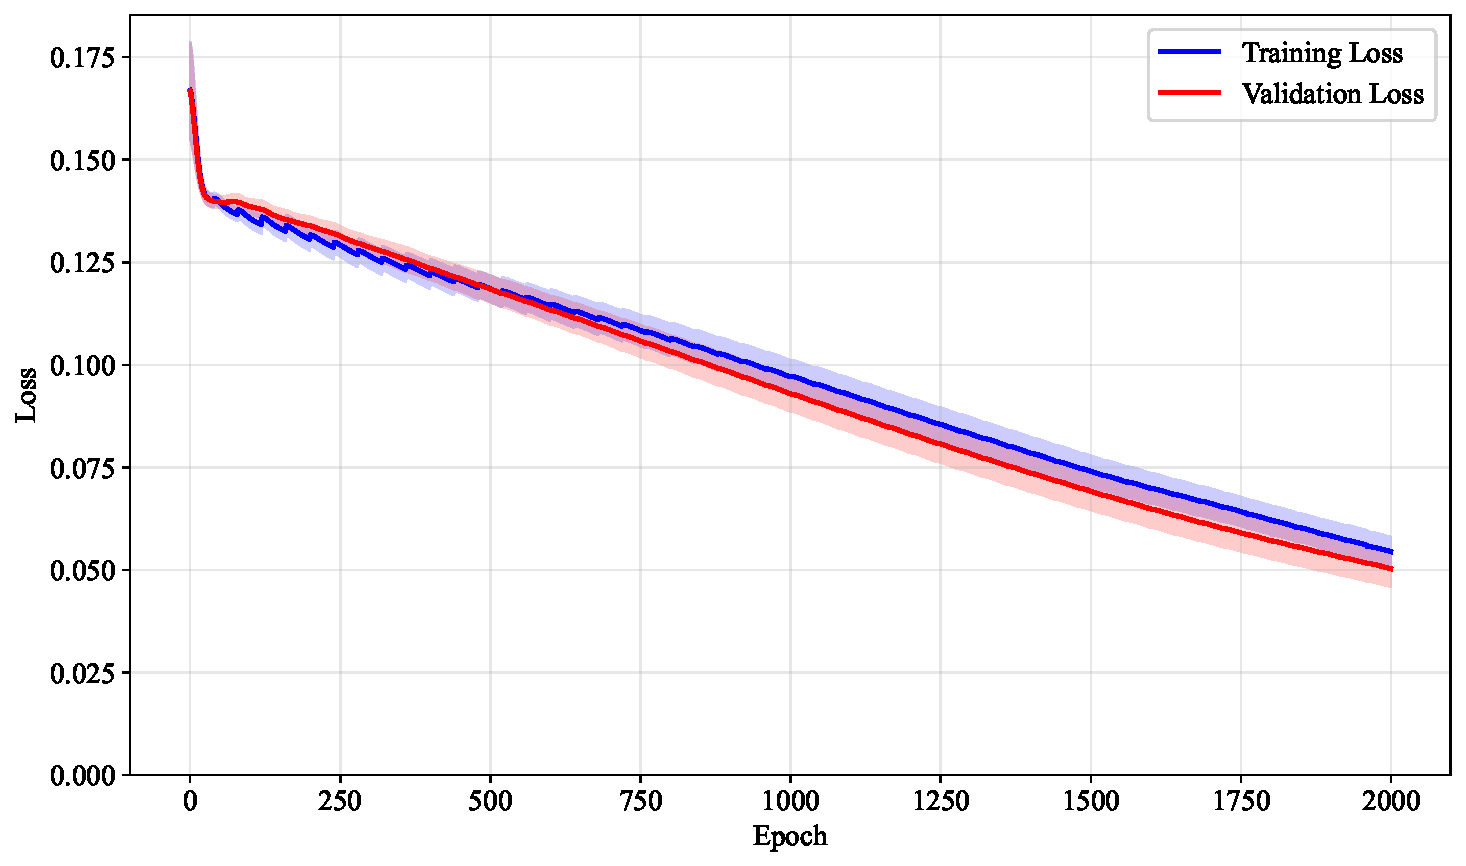
\includegraphics[width=\linewidth]{../results/wine/us_losses.pdf}
		\caption{Entropy uncertainty sampling losses.}
		\label{fig:us_losses_wine}
	\end{subfigure}
	
	\vspace{0.1em}
	
	\begin{subfigure}{\linewidth}
		\centering
		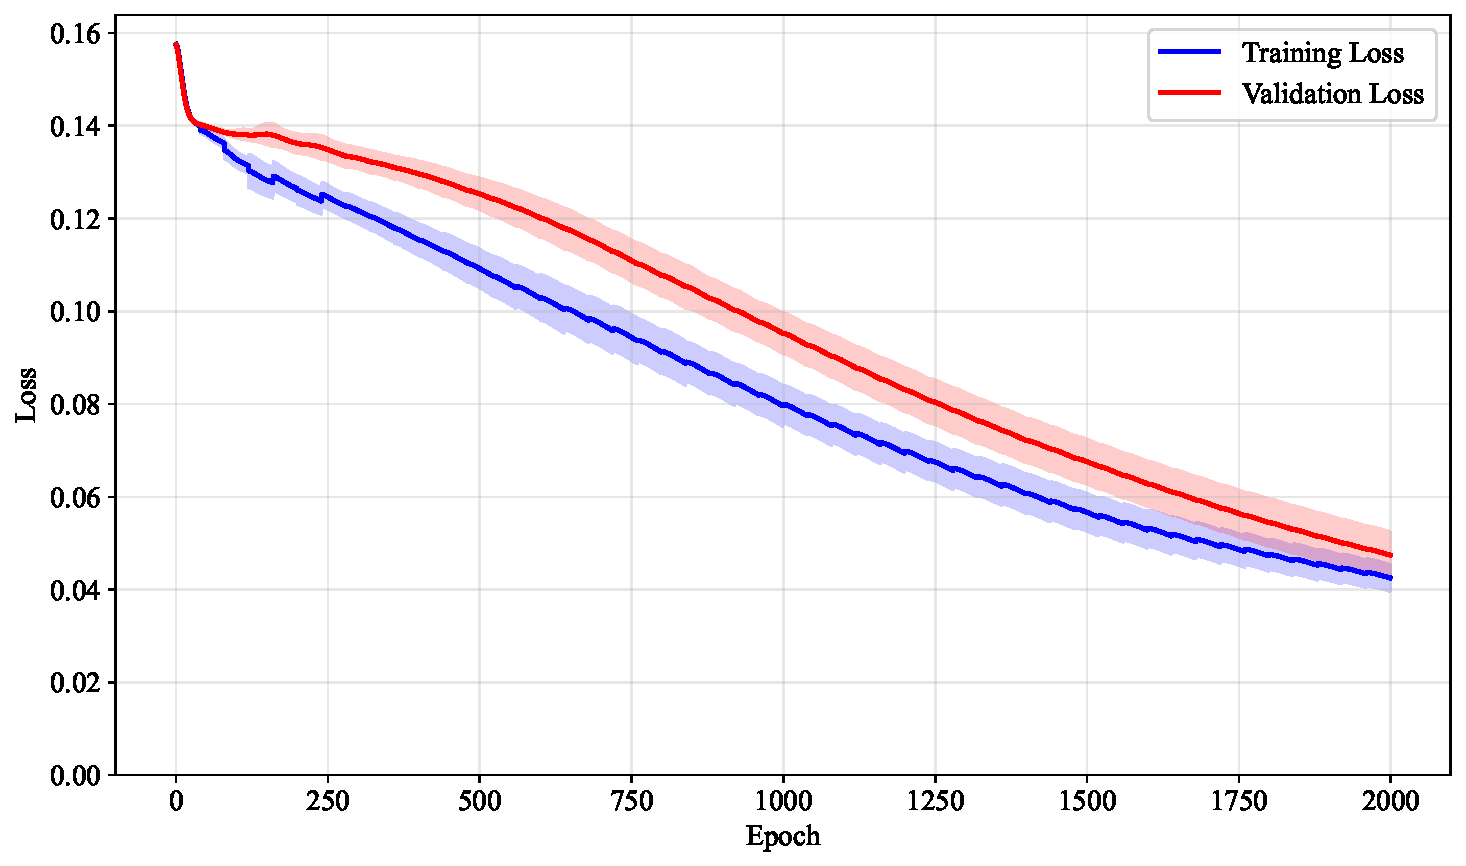
\includegraphics[width=\linewidth]{../results/wine/ensemble_us_losses.pdf}
		\caption{Ensemble uncertainty sampling losses.}
		\label{fig:ensemble_us_losses_wine}
	\end{subfigure}
\end{figure}


\begin{figure}[!t]
	\centering
	\caption{Losses for training of frameworks with the fashion-MNIST dataset.}
	\label{fig:fashion-loss}
	\begin{subfigure}{\linewidth}
		\centering
		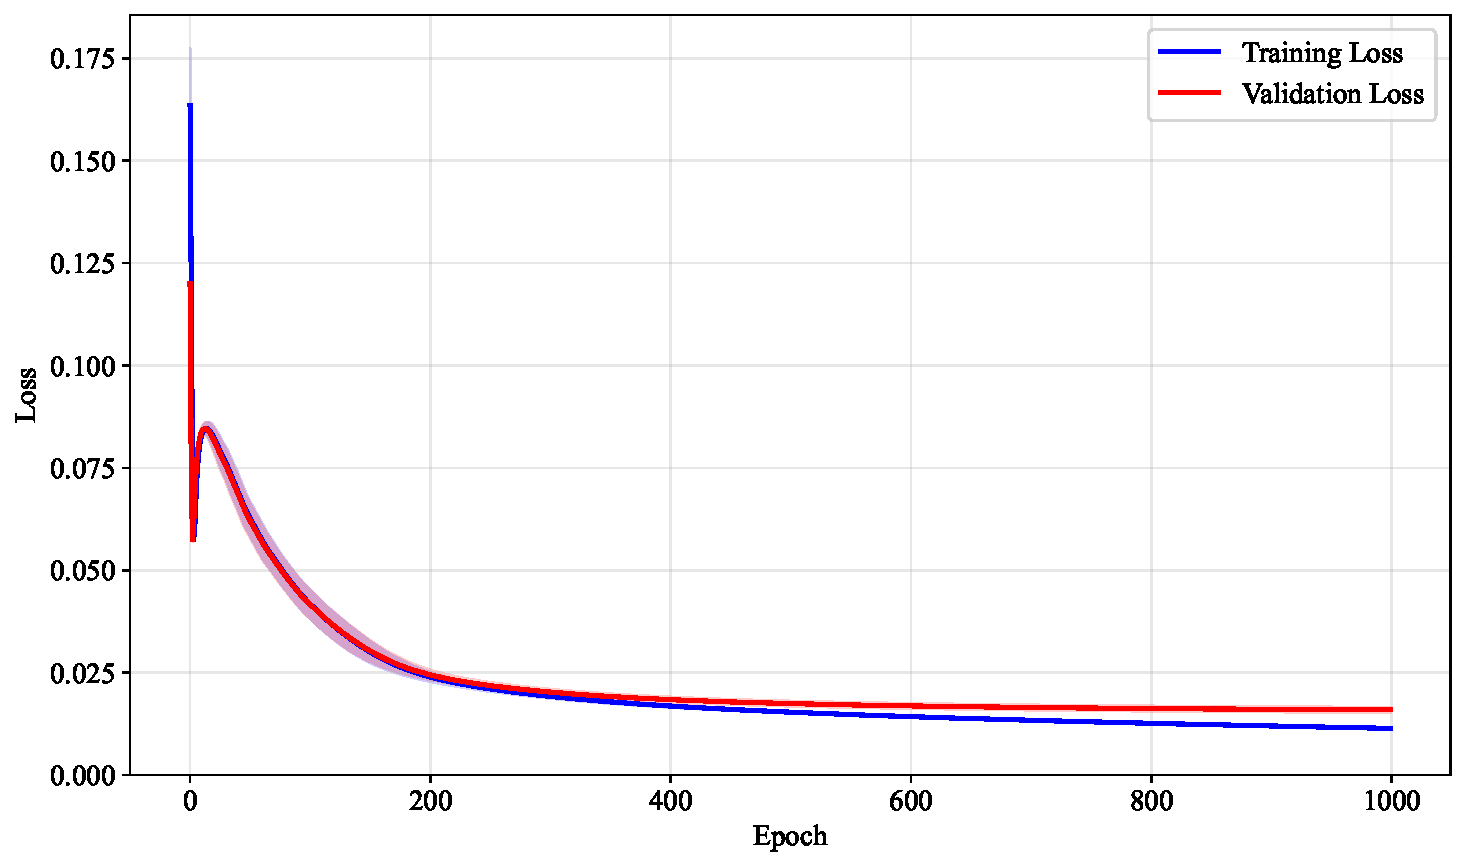
\includegraphics[width=\linewidth]{../results/fashion/losses.pdf}
		\caption{Passive learning losses.}
		\label{fig:losses_fashion}
	\end{subfigure}
	
	\vspace{0.1em}
	
	\begin{subfigure}{\linewidth}
		\centering
		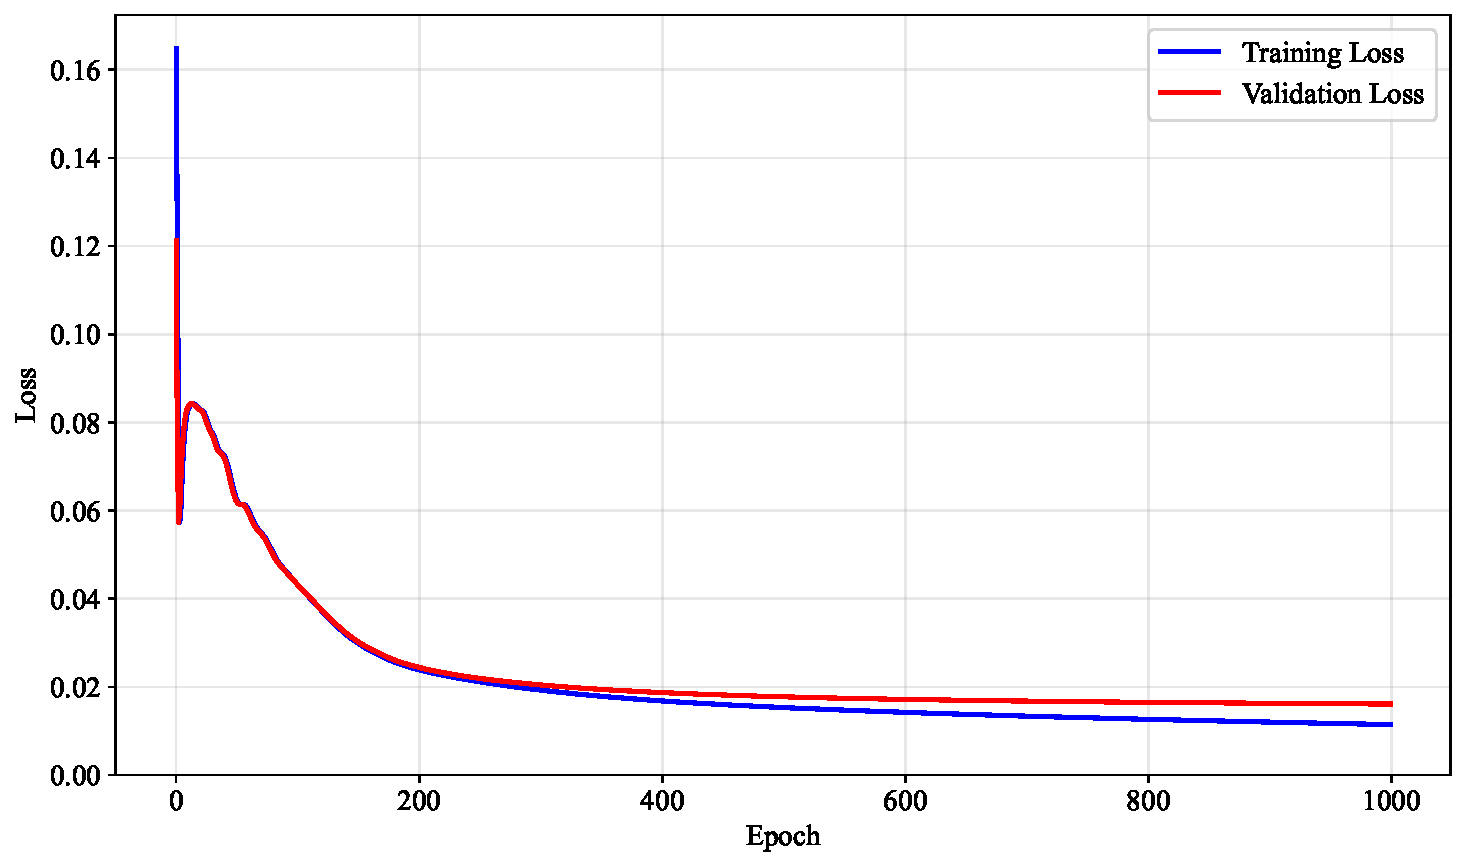
\includegraphics[width=\linewidth]{../results/fashion/os_losses.pdf}
		\caption{SASLA losses.}
		\label{fig:os_losses_fashion}
	\end{subfigure}
	
	\vspace{0.1em}
	
	\begin{subfigure}{\linewidth}
		\centering
		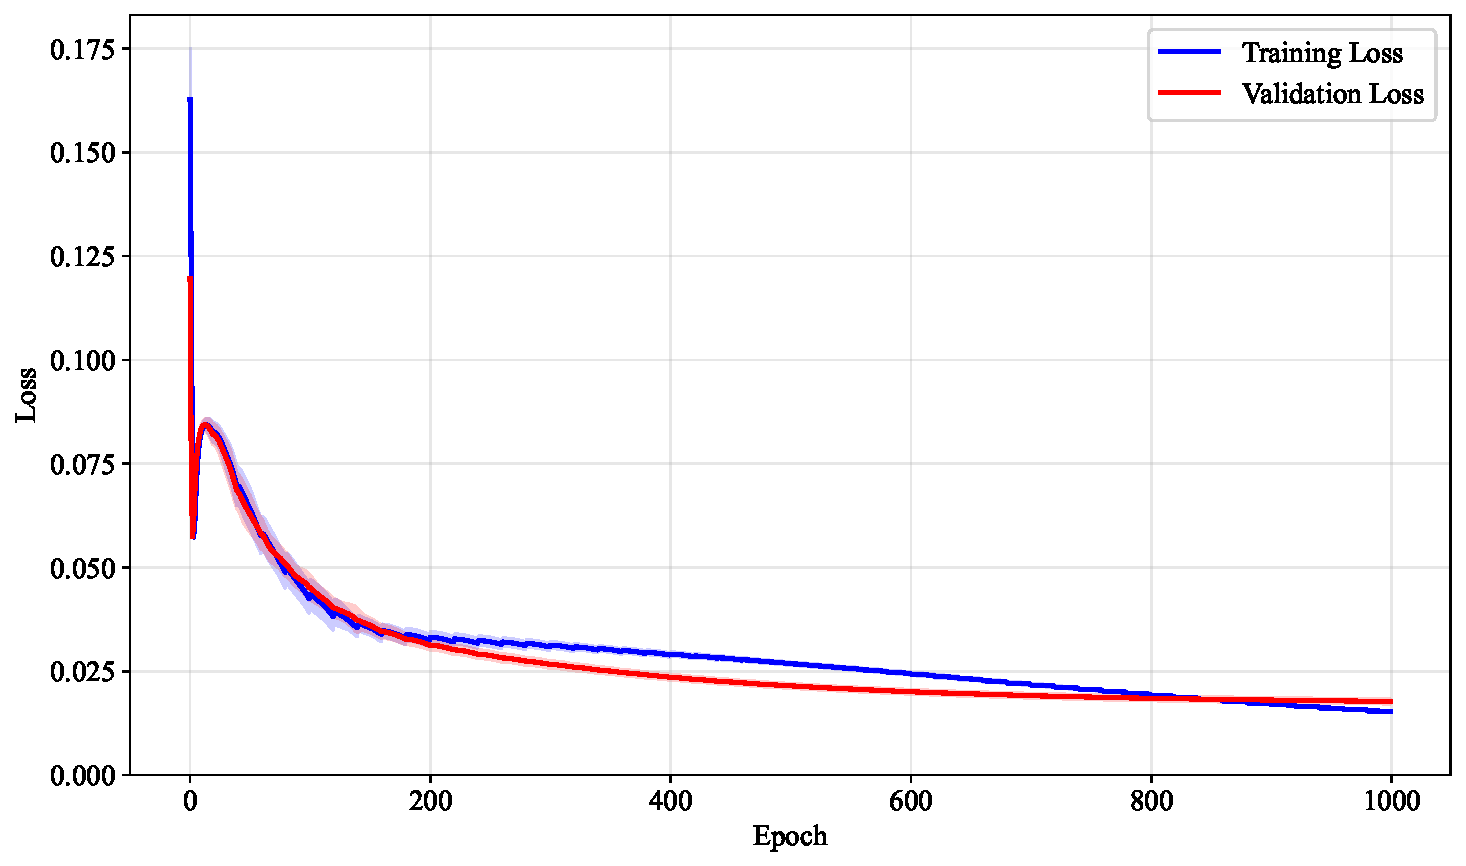
\includegraphics[width=\linewidth]{../results/fashion/us_losses.pdf}
		\caption{Entropy uncertainty sampling losses.}
		\label{fig:us_losses_fashion}
	\end{subfigure}
	
	\vspace{0.1em}
	
	\begin{subfigure}{\linewidth}
		\centering
		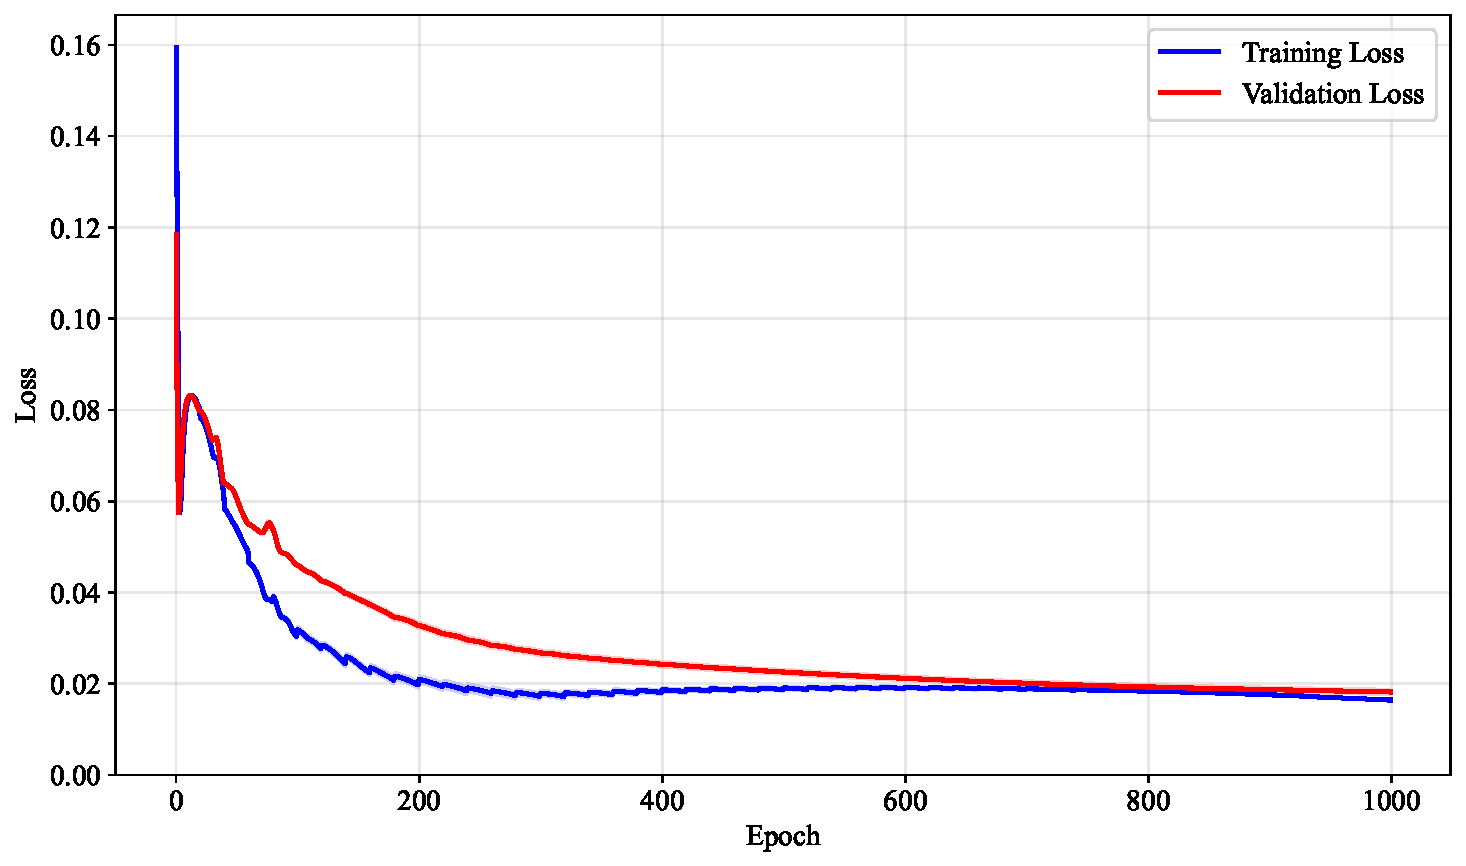
\includegraphics[width=\linewidth]{../results/fashion/ensemble_us_losses.pdf}
		\caption{Ensemble uncertainty sampling losses.}
		\label{fig:ensemble_us_losses_fashion}
	\end{subfigure}
\end{figure}


\begin{figure}[!t]
	\centering
	\caption{Losses for training of frameworks with the synthetic function dataset.}
	
	\begin{subfigure}{\linewidth}
		\centering
		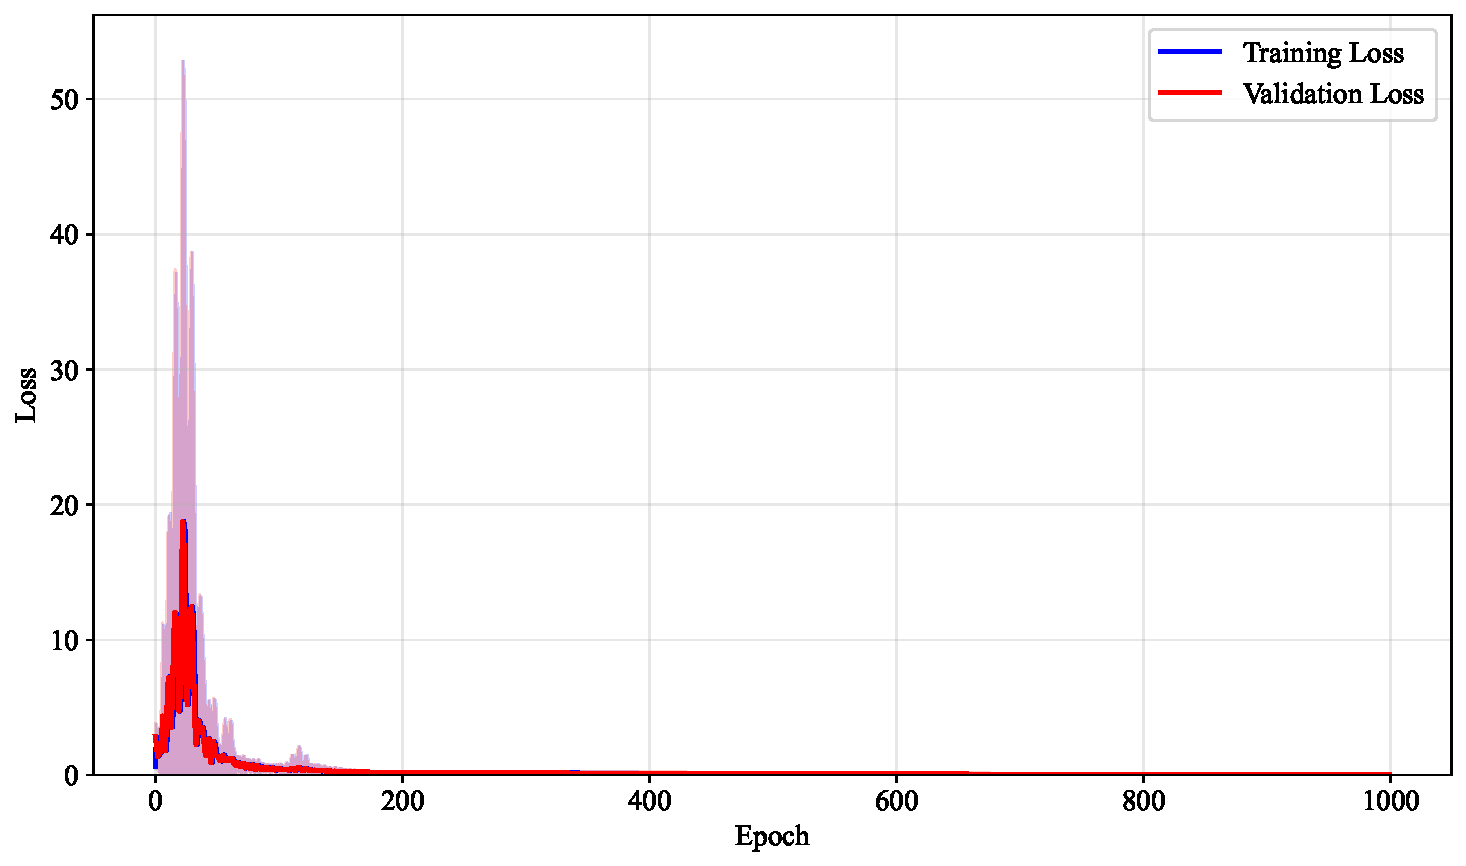
\includegraphics[width=\linewidth]{../results/synfunc/losses.pdf}
		\caption{Passive learning losses.}
		\label{fig:losses_synfunc}
	\end{subfigure}
	
	\vspace{0.1em}
	
	\begin{subfigure}{\linewidth}
		\centering
		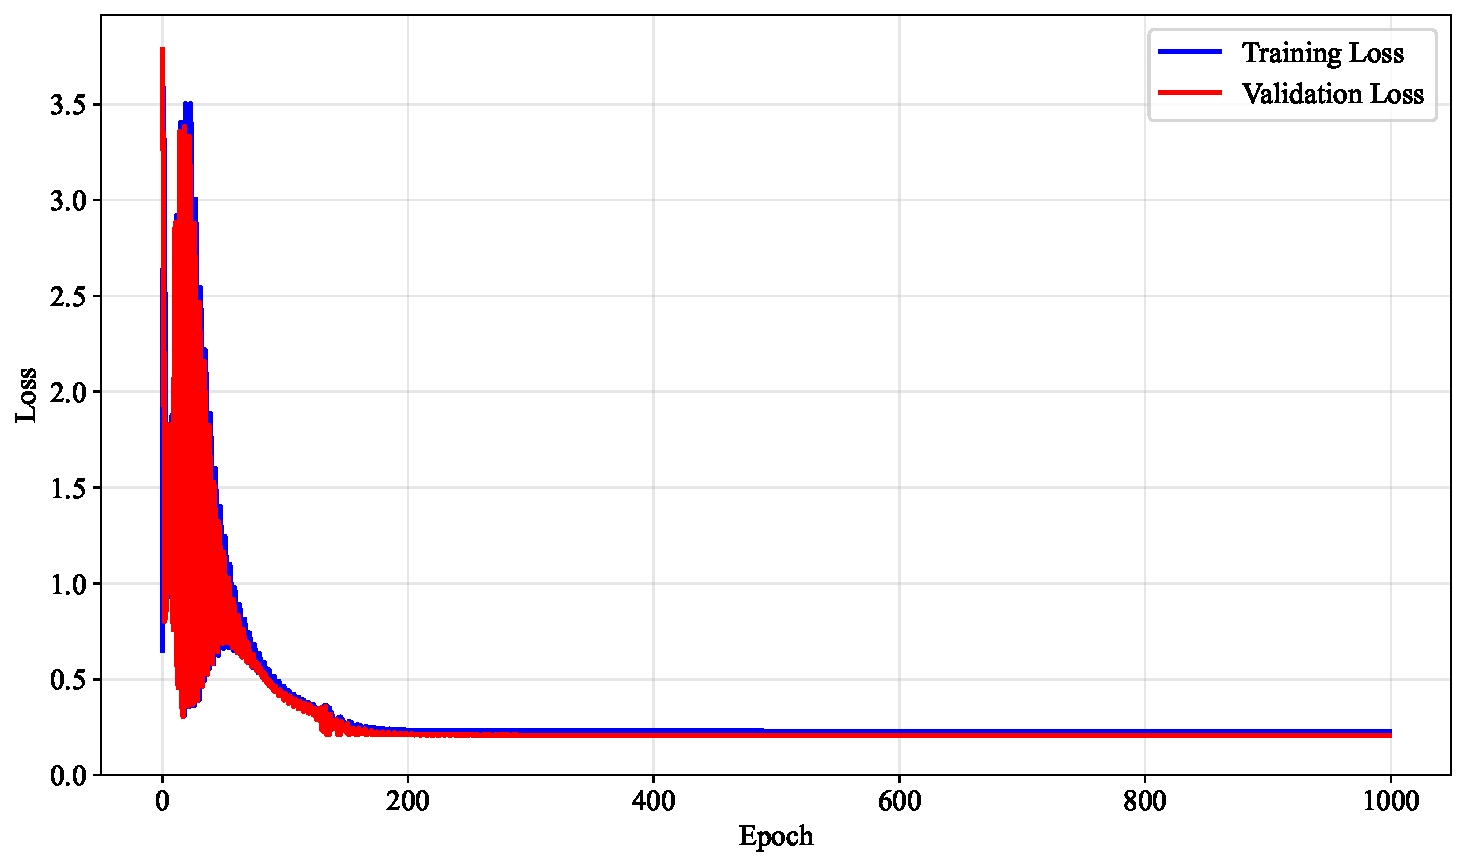
\includegraphics[width=\linewidth]{../results/synfunc/os_losses.pdf}
		\caption{SASLA losses.}
		\label{fig:os_losses_synfunc}
	\end{subfigure}
	
	\vspace{0.1em}
	
	\begin{subfigure}{\linewidth}
		\centering
		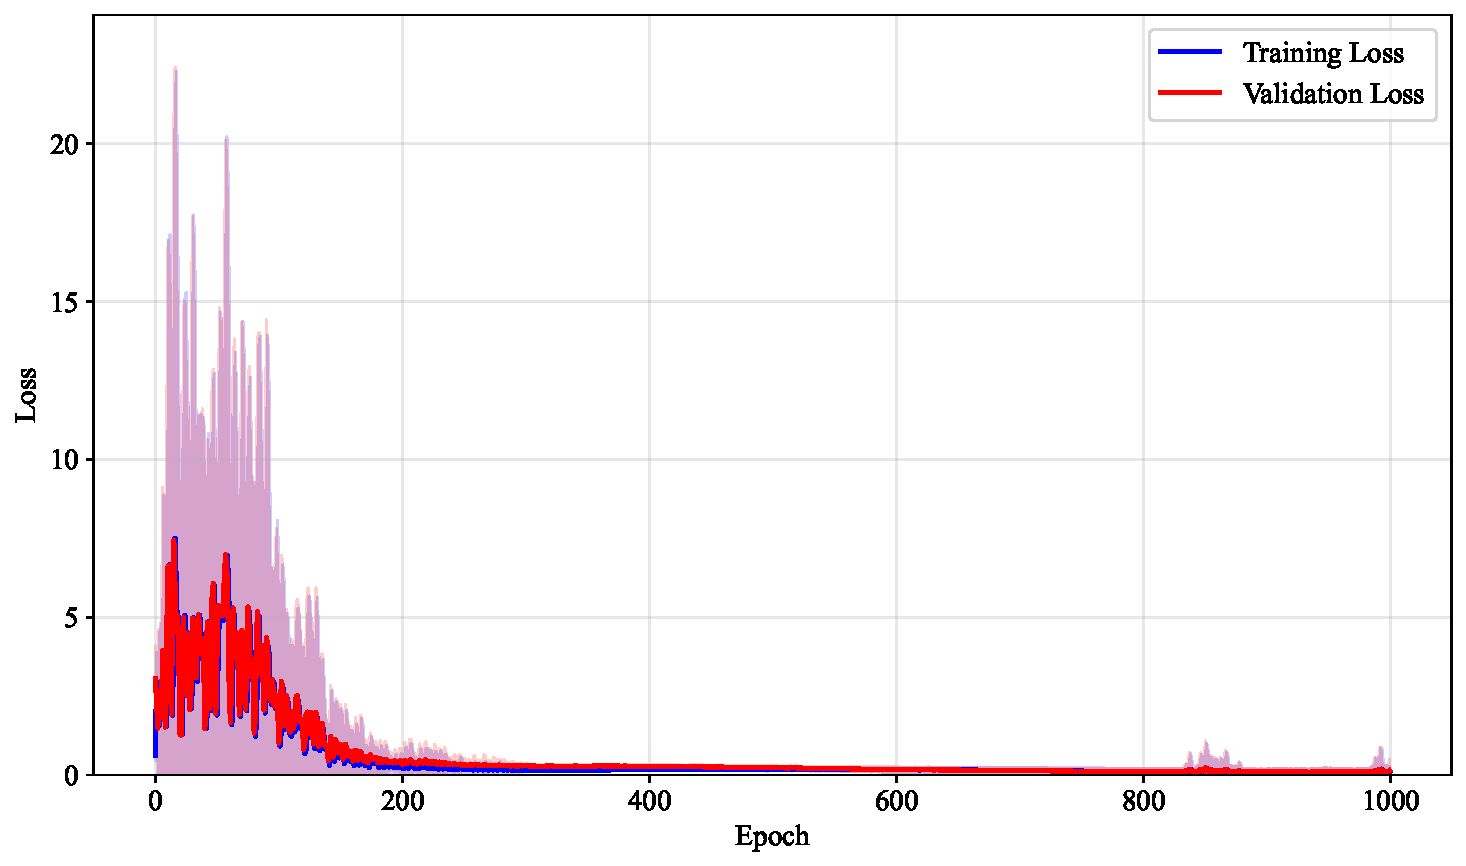
\includegraphics[width=\linewidth]{../results/synfunc/us_losses.pdf}
		\caption{Entropy uncertainty sampling losses.}
		\label{fig:us_losses_synfunc}
	\end{subfigure}
	
	\vspace{0.1em}
	
	\begin{subfigure}{\linewidth}
		\centering
		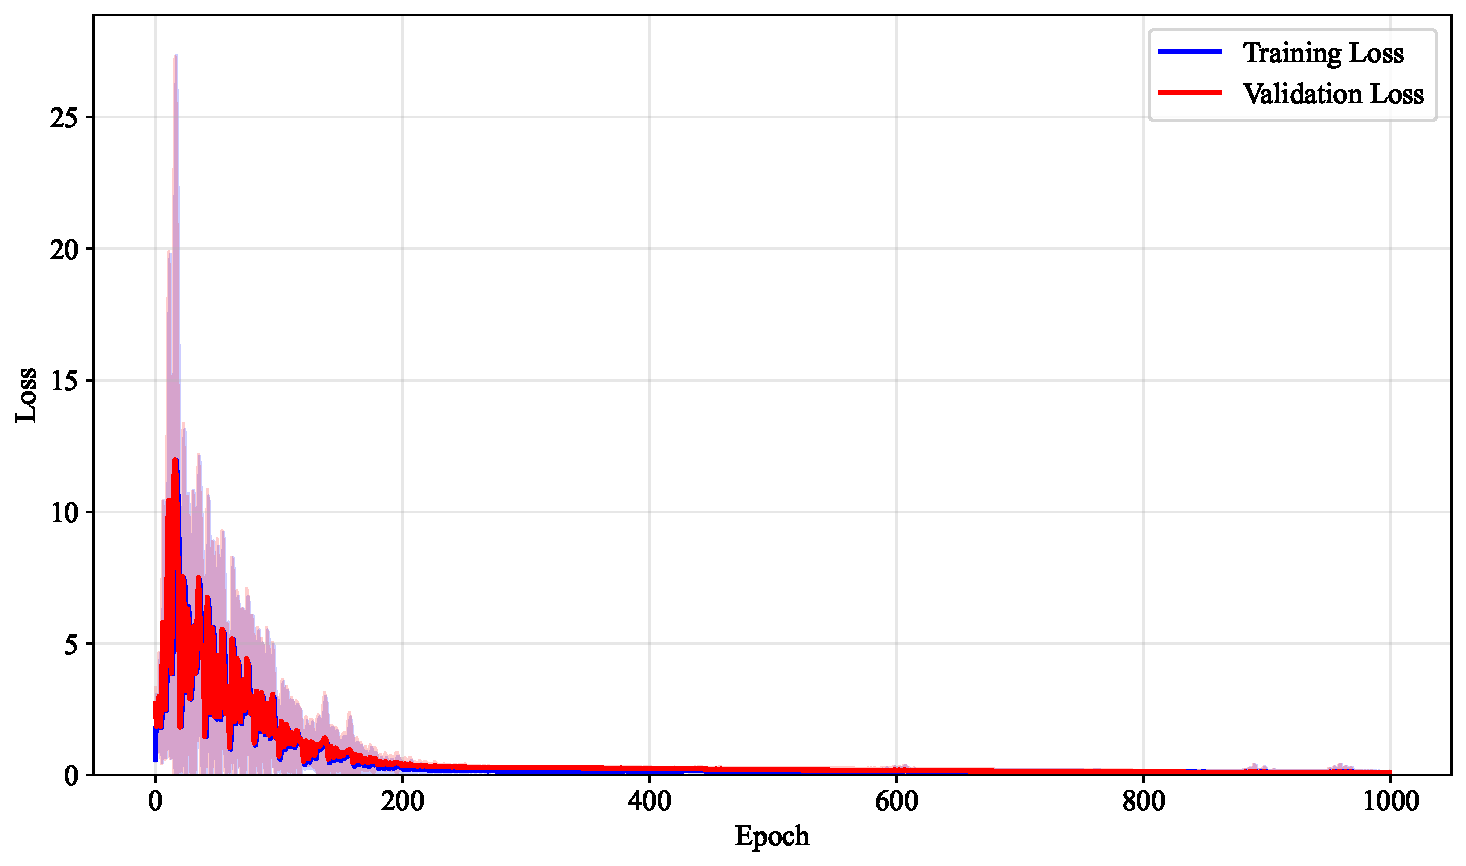
\includegraphics[width=\linewidth]{../results/synfunc/ensemble_us_losses.pdf}
		\caption{Ensemble uncertainty sampling losses.}
		\label{fig:ensemble_us_losses_synfunc}
	\end{subfigure}
\end{figure}

\begin{figure}[!t]
	\centering
	\caption{Losses for training of frameworks with the California housing dataset.}
	
	\begin{subfigure}{\linewidth}
		\centering
		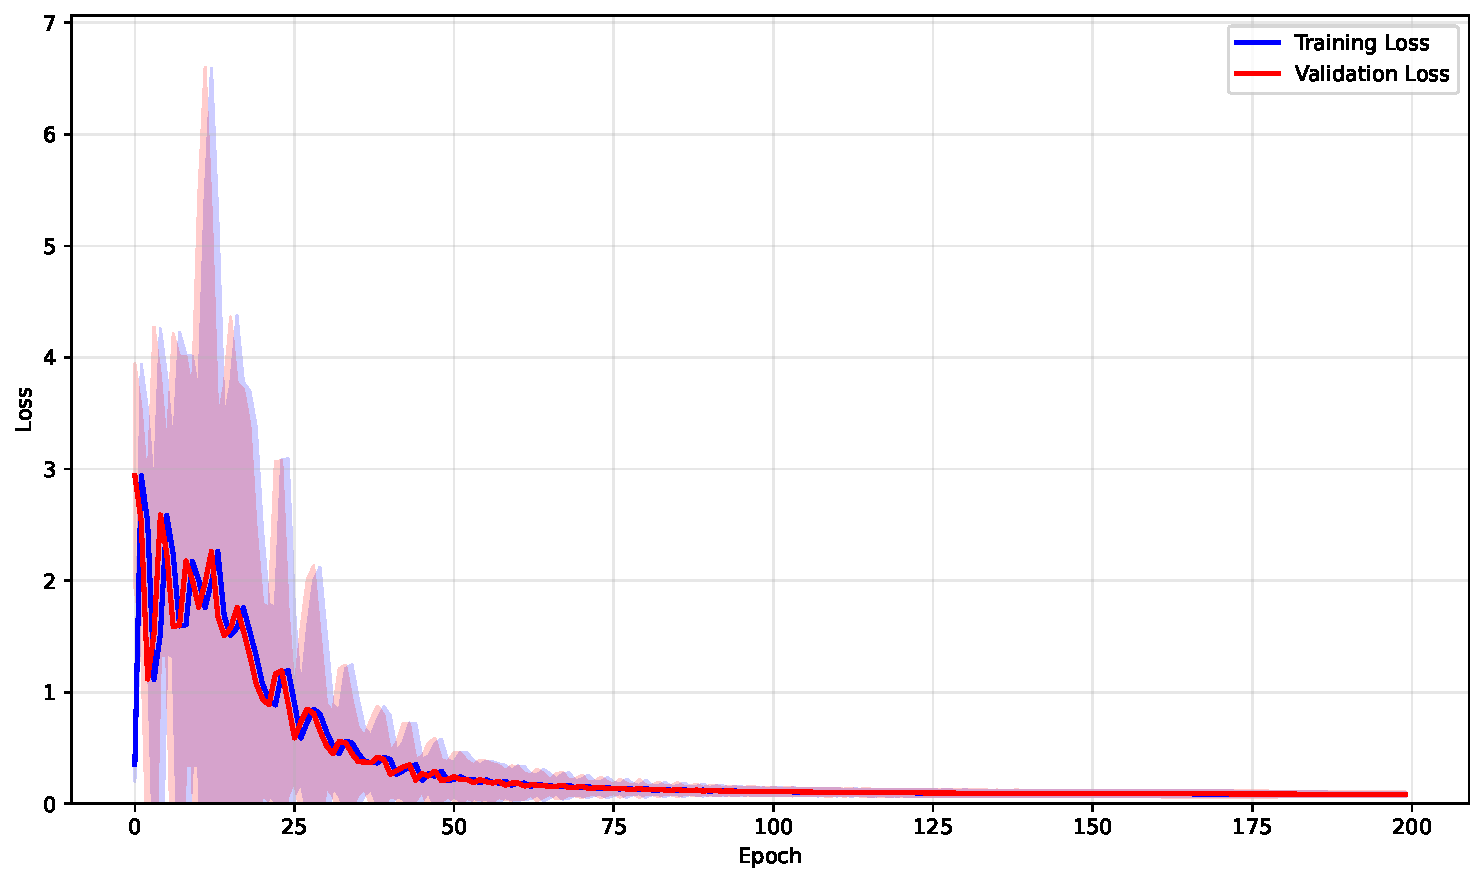
\includegraphics[width=\linewidth]{../results/housing/losses.pdf}
		\caption{Passive learning losses.}
		\label{fig:losses_housing}
	\end{subfigure}
	
	\vspace{0.1em}
	
	\begin{subfigure}{\linewidth}
		\centering
		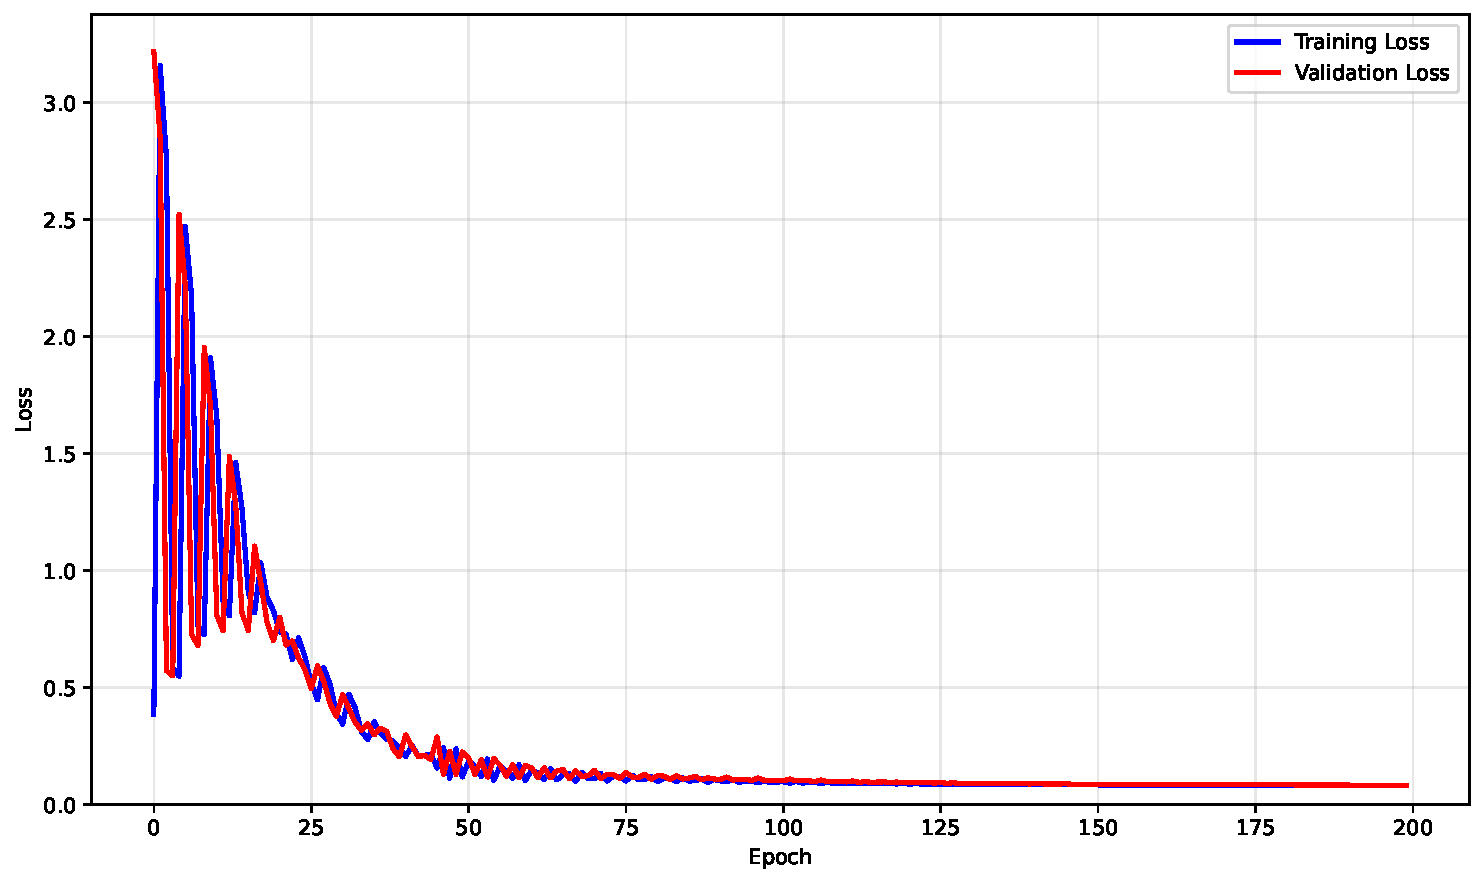
\includegraphics[width=\linewidth]{../results/housing/os_losses.pdf}
		\caption{SASLA losses.}
		\label{fig:os_losses_housing}
	\end{subfigure}
	
	\vspace{0.1em}
	
	\begin{subfigure}{\linewidth}
		\centering
		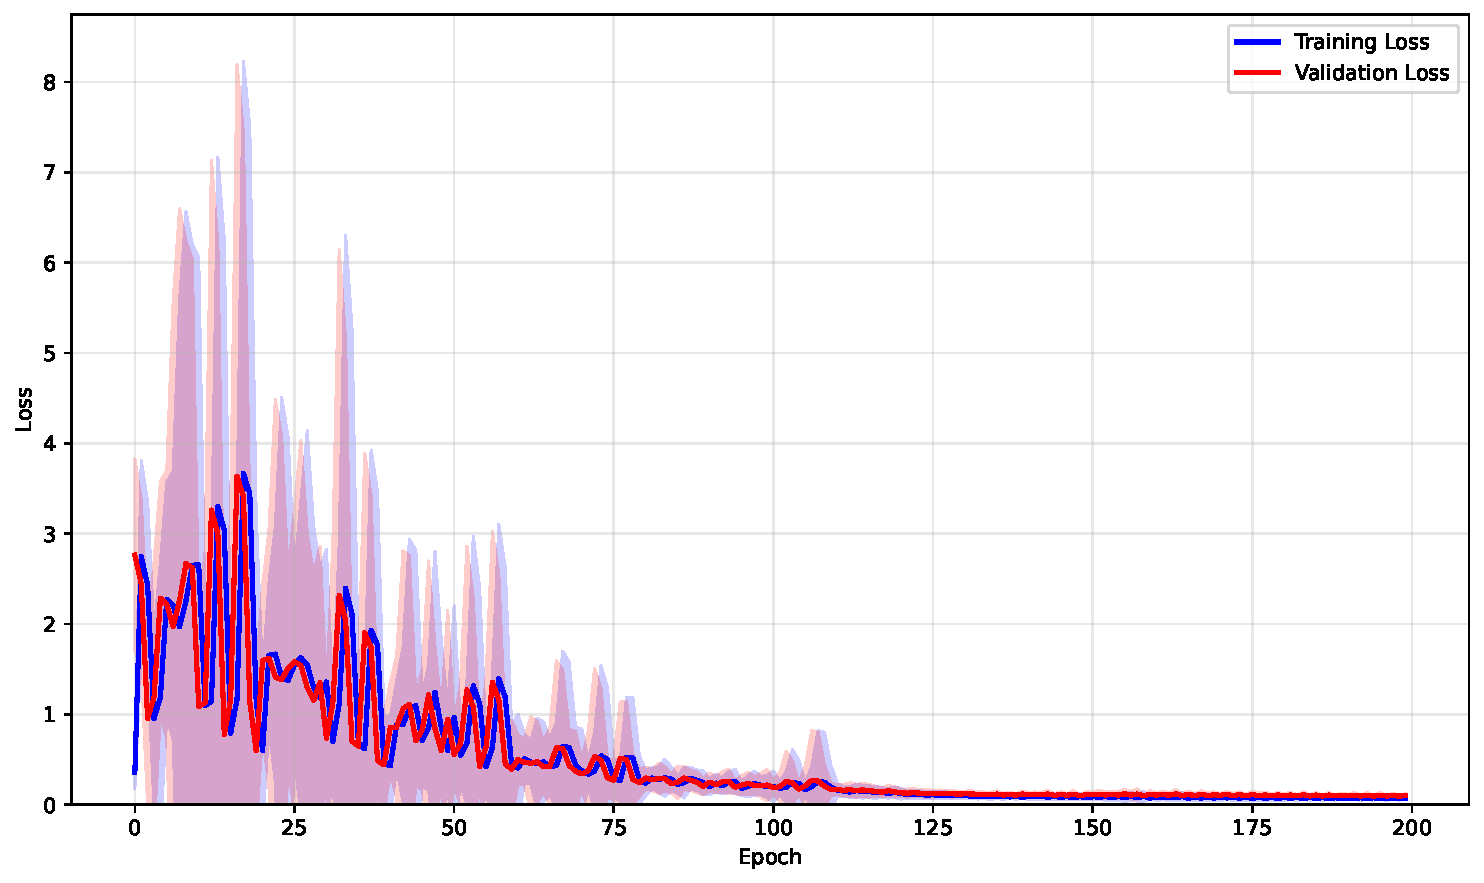
\includegraphics[width=\linewidth]{../results/housing/us_losses.pdf}
		\caption{Entropy uncertainty sampling losses.}
		\label{fig:us_losses_housing}
	\end{subfigure}
	
	\vspace{0.1em}
	
	\begin{subfigure}{\linewidth}
		\centering
		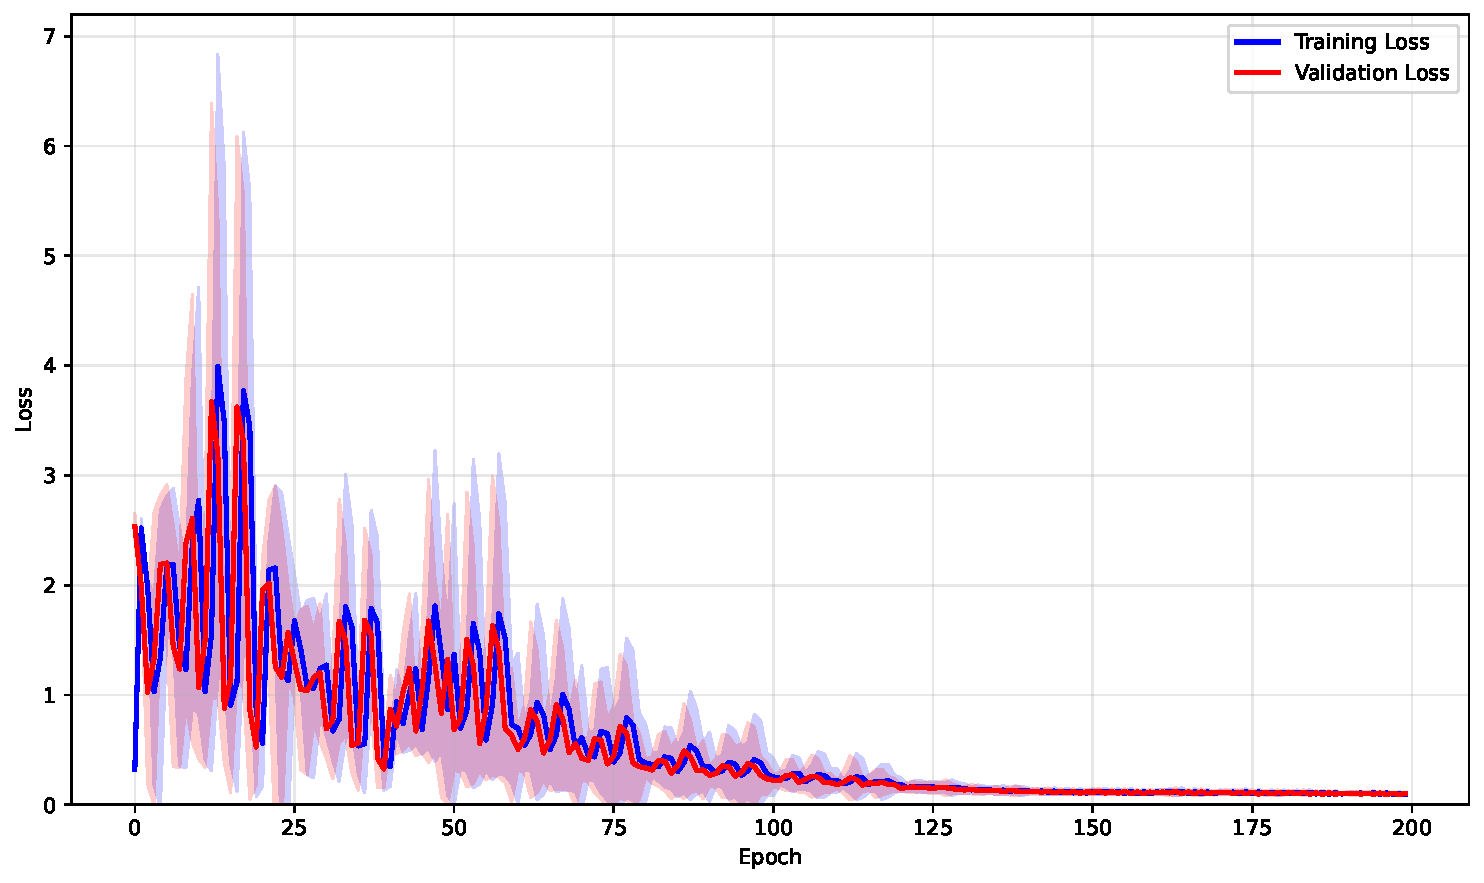
\includegraphics[width=\linewidth]{../results/housing/ensemble_us_losses.pdf}
		\caption{Ensemble uncertainty sampling losses.}
		\label{fig:ensemble_us_losses_housing}
	\end{subfigure}
\end{figure}

\begin{figure}[!t]
	\centering
	\caption{Losses for training of frameworks with the energy efficiency dataset.}
	
	\begin{subfigure}{\linewidth}
		\centering
		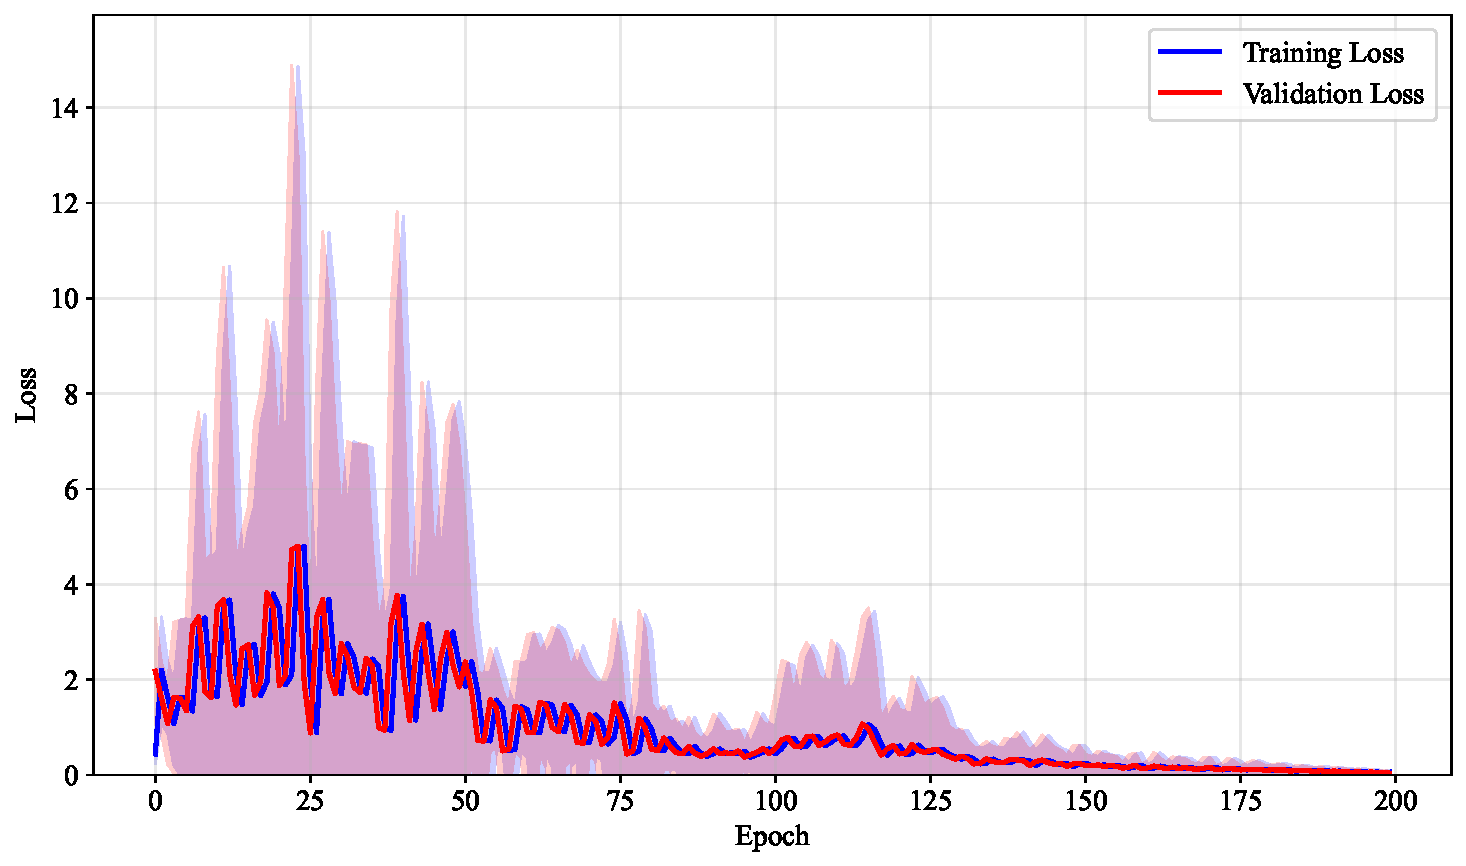
\includegraphics[width=\linewidth]{../results/energy/losses.pdf}
		\caption{Passive learning losses.}
		\label{fig:losses_energy}
	\end{subfigure}
	
	\vspace{0.1em}
	
	\begin{subfigure}{\linewidth}
		\centering
		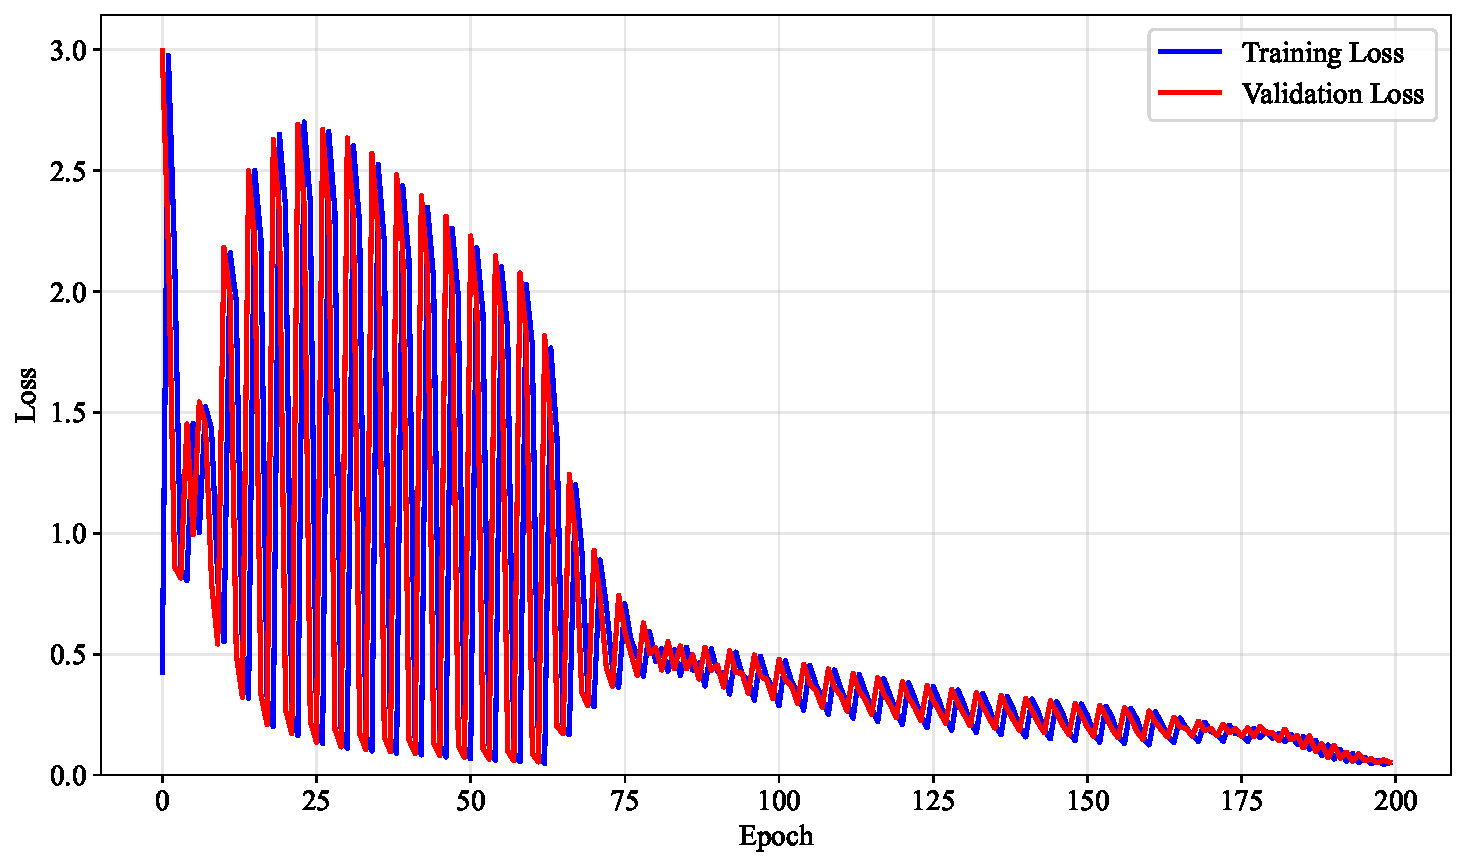
\includegraphics[width=\linewidth]{../results/energy/os_losses.pdf}
		\caption{SASLA losses.}
		\label{fig:os_losses_energy}
	\end{subfigure}
	
	\vspace{0.1em}
	
	\begin{subfigure}{\linewidth}
		\centering
		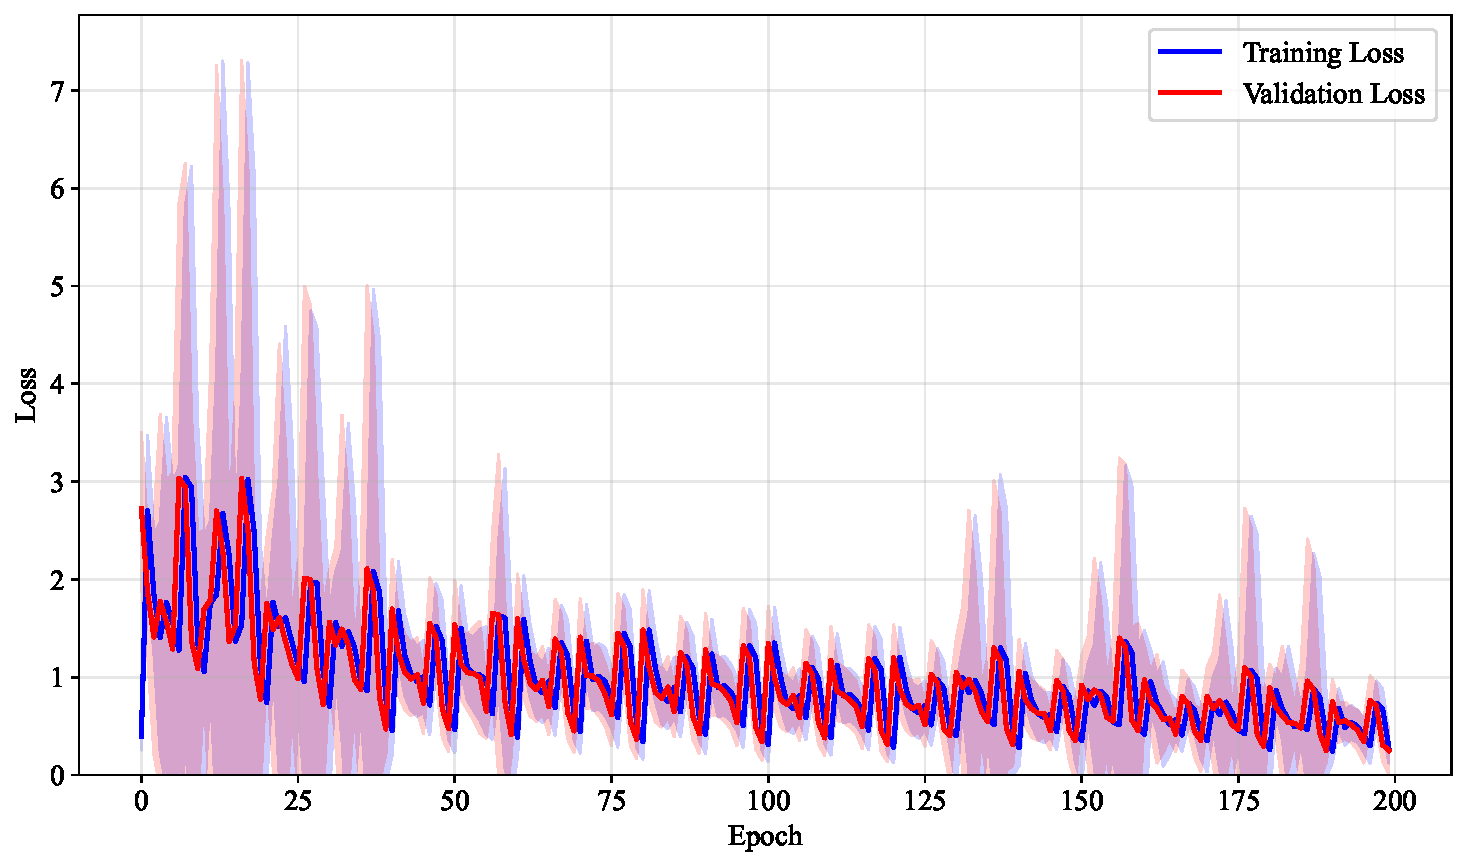
\includegraphics[width=\linewidth]{../results/energy/us_losses.pdf}
		\caption{Entropy uncertainty sampling losses.}
		\label{fig:us_losses_energy}
	\end{subfigure}
	
	\vspace{0.1em}
	
	\begin{subfigure}{\linewidth}
		\centering
		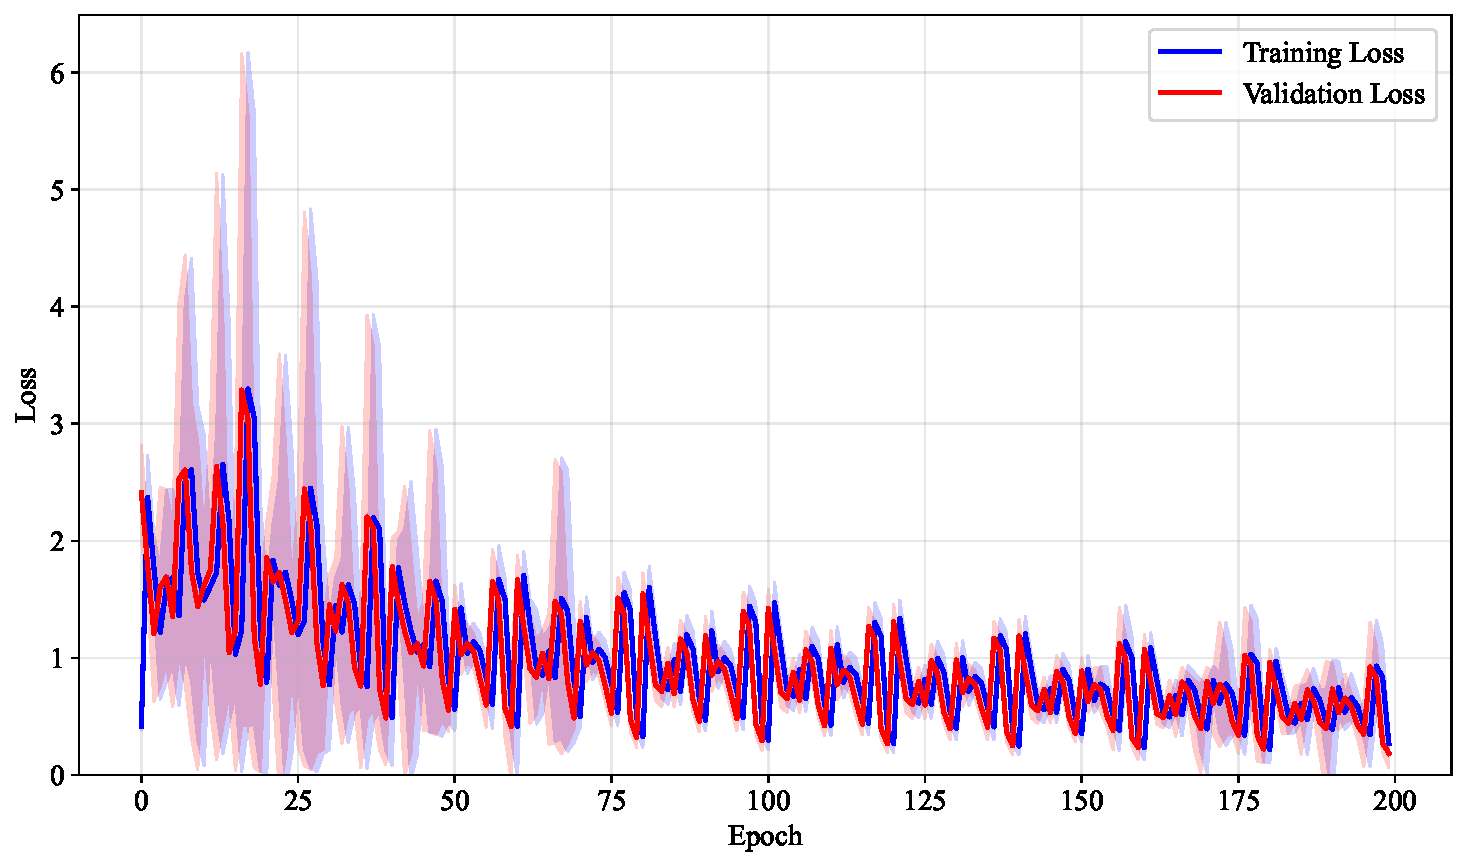
\includegraphics[width=\linewidth]{../results/energy/ensemble_us_losses.pdf}
		\caption{Ensemble uncertainty sampling losses.}
		\label{fig:ensemble_us_losses_energy}
	\end{subfigure}
\end{figure}

\begin{figure}[!t]
	\centering
	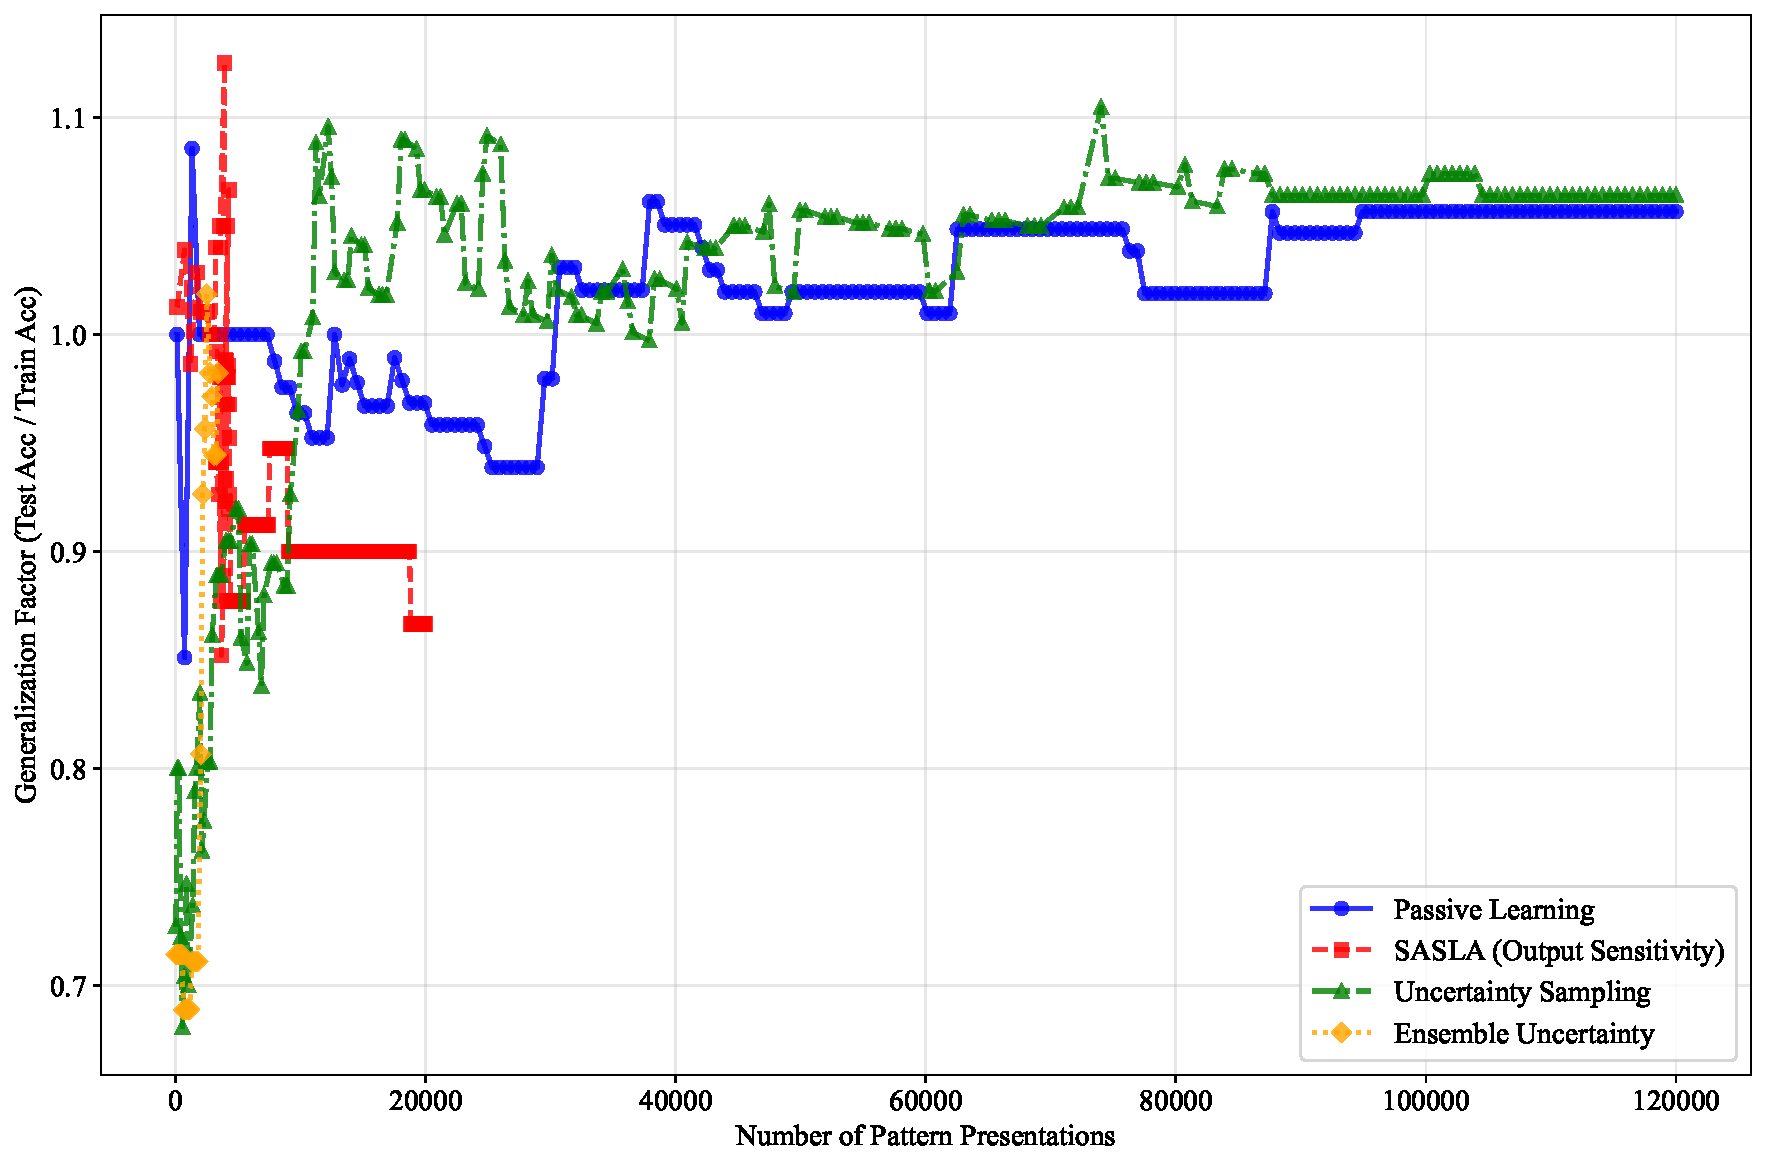
\includegraphics[width=\linewidth]{../results/iris/generalization_factor_vs_presentations.pdf}
	\caption{Generalisation factor versus number of pattern presentations for the iris dataset.}
	\label{fig:gf_iris}
\end{figure}

\begin{figure}[!t]
	\centering
	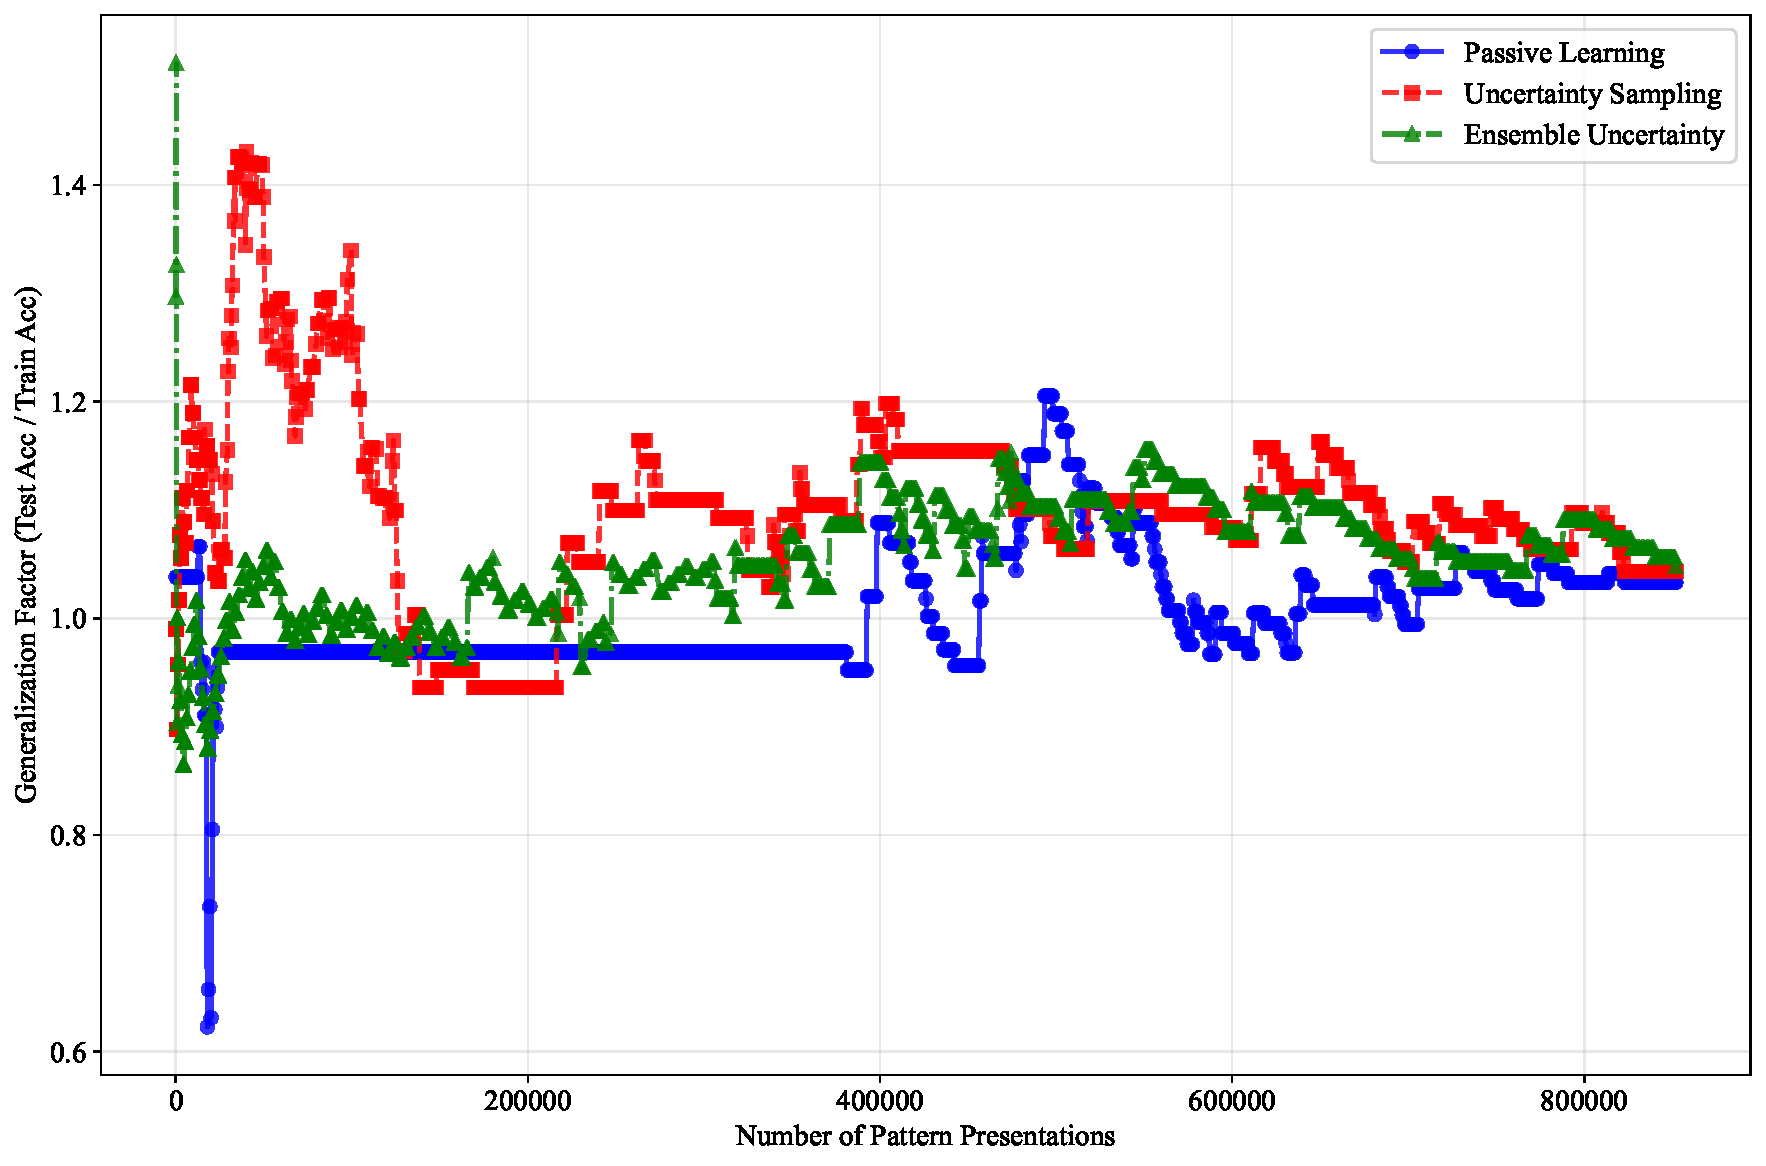
\includegraphics[width=\linewidth]{../results/wine/generalization_factor_vs_presentations.pdf}
	\caption{Generalisation factor versus number of pattern presentations for the wine dataset.}
	\label{fig:gf_wine}
\end{figure}

\begin{figure}[!t]
	\centering
	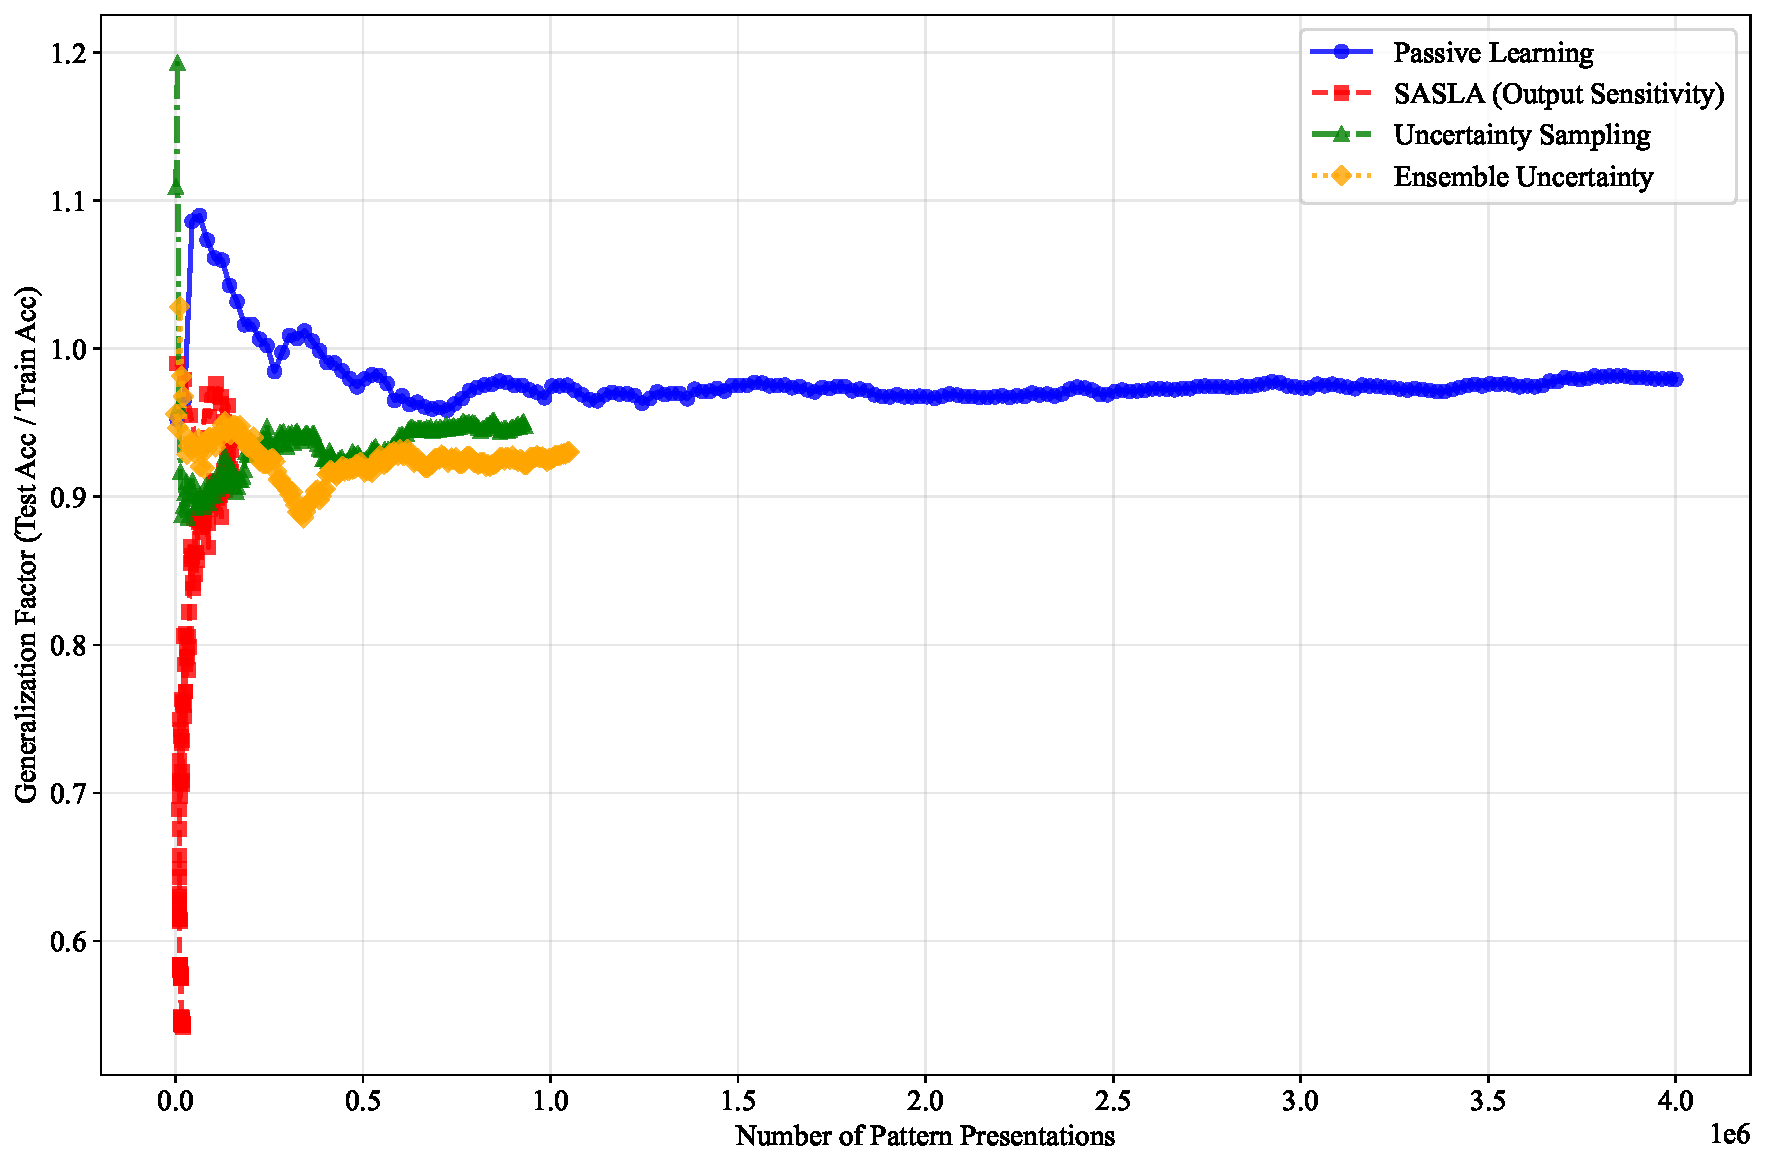
\includegraphics[width=\linewidth]{../results/fashion/generalization_factor_vs_presentations.pdf}
	\caption{Generalisation factor versus number of pattern presentations for the fashion-MNIST dataset.}
	\label{fig:gf_fashion}
\end{figure}

\begin{figure}[!t]
	\centering
	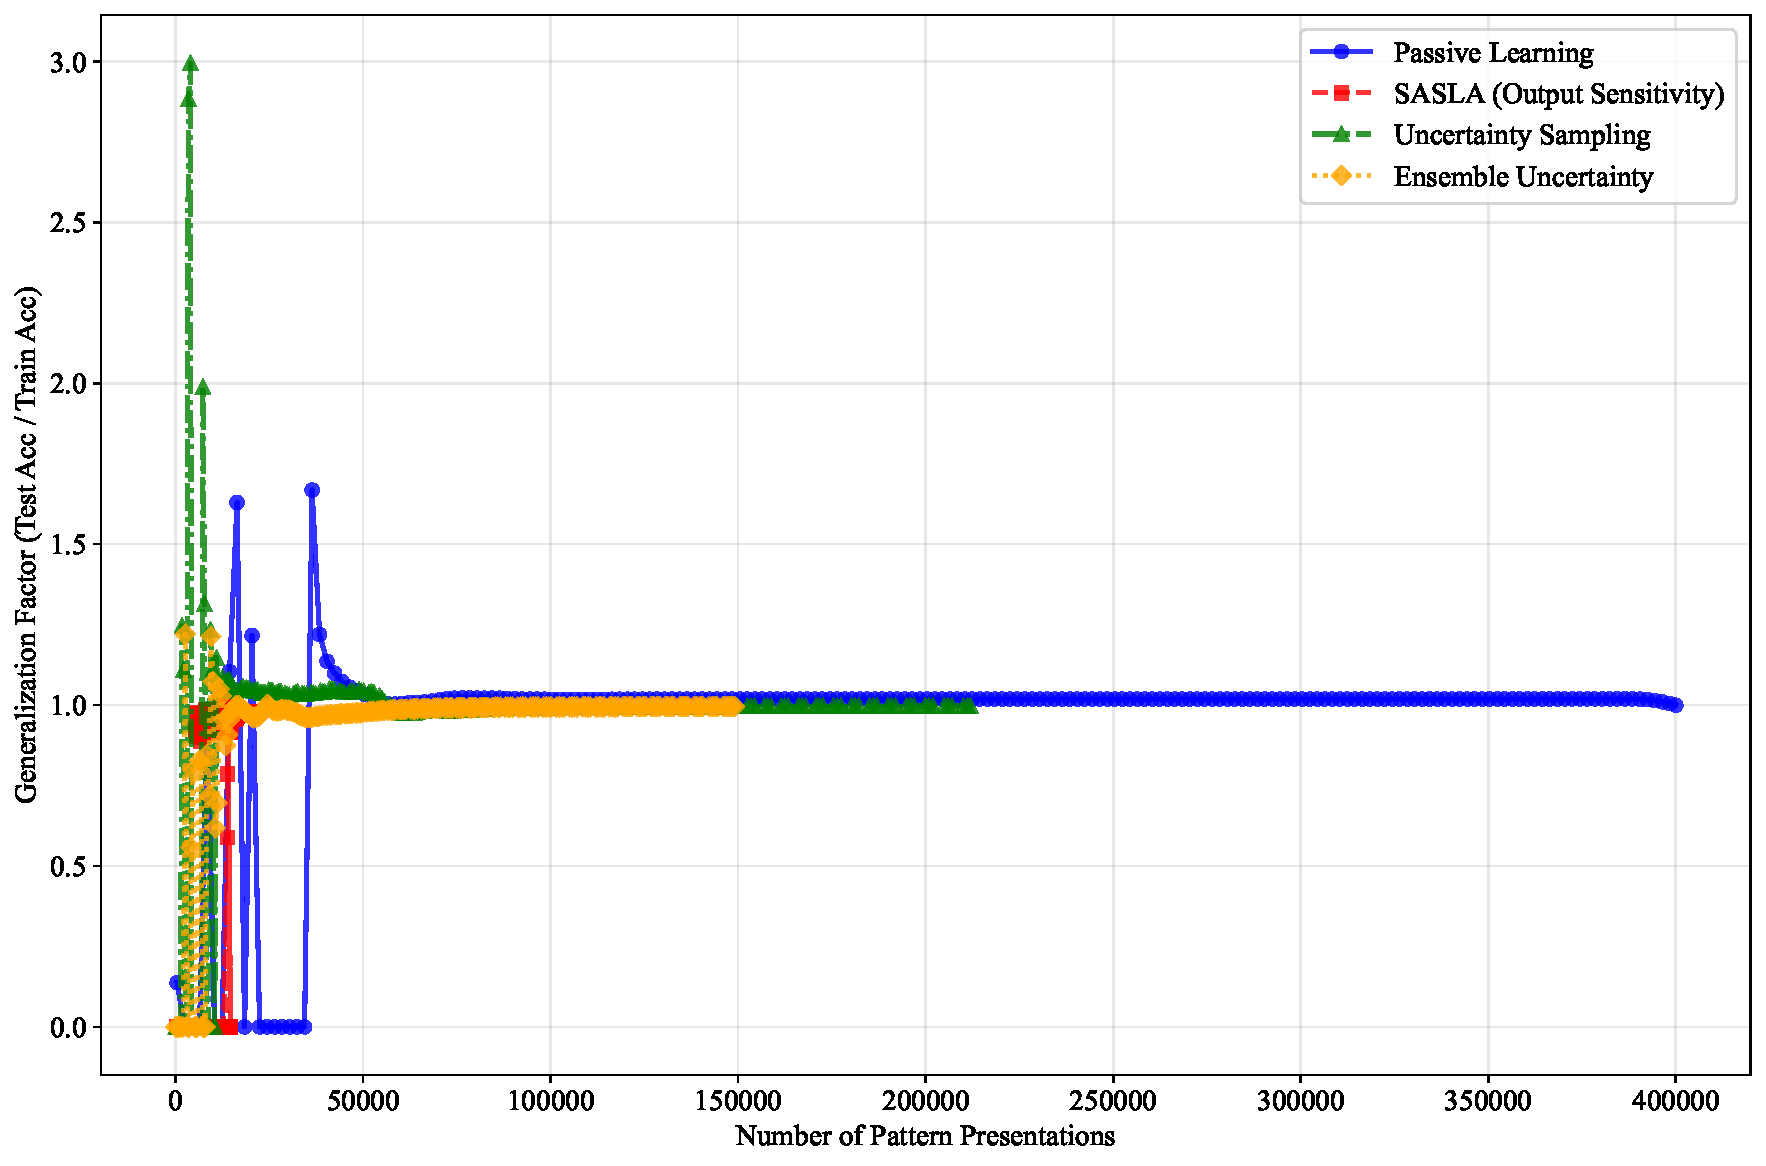
\includegraphics[width=\linewidth]{../results/synfunc/generalization_factor_vs_presentations.pdf}
	\caption{Generalisation factor versus number of pattern presentations for the synthetic function dataset.}
	\label{fig:gf_synfunc}
\end{figure}

\begin{figure}[!t]
	\centering
	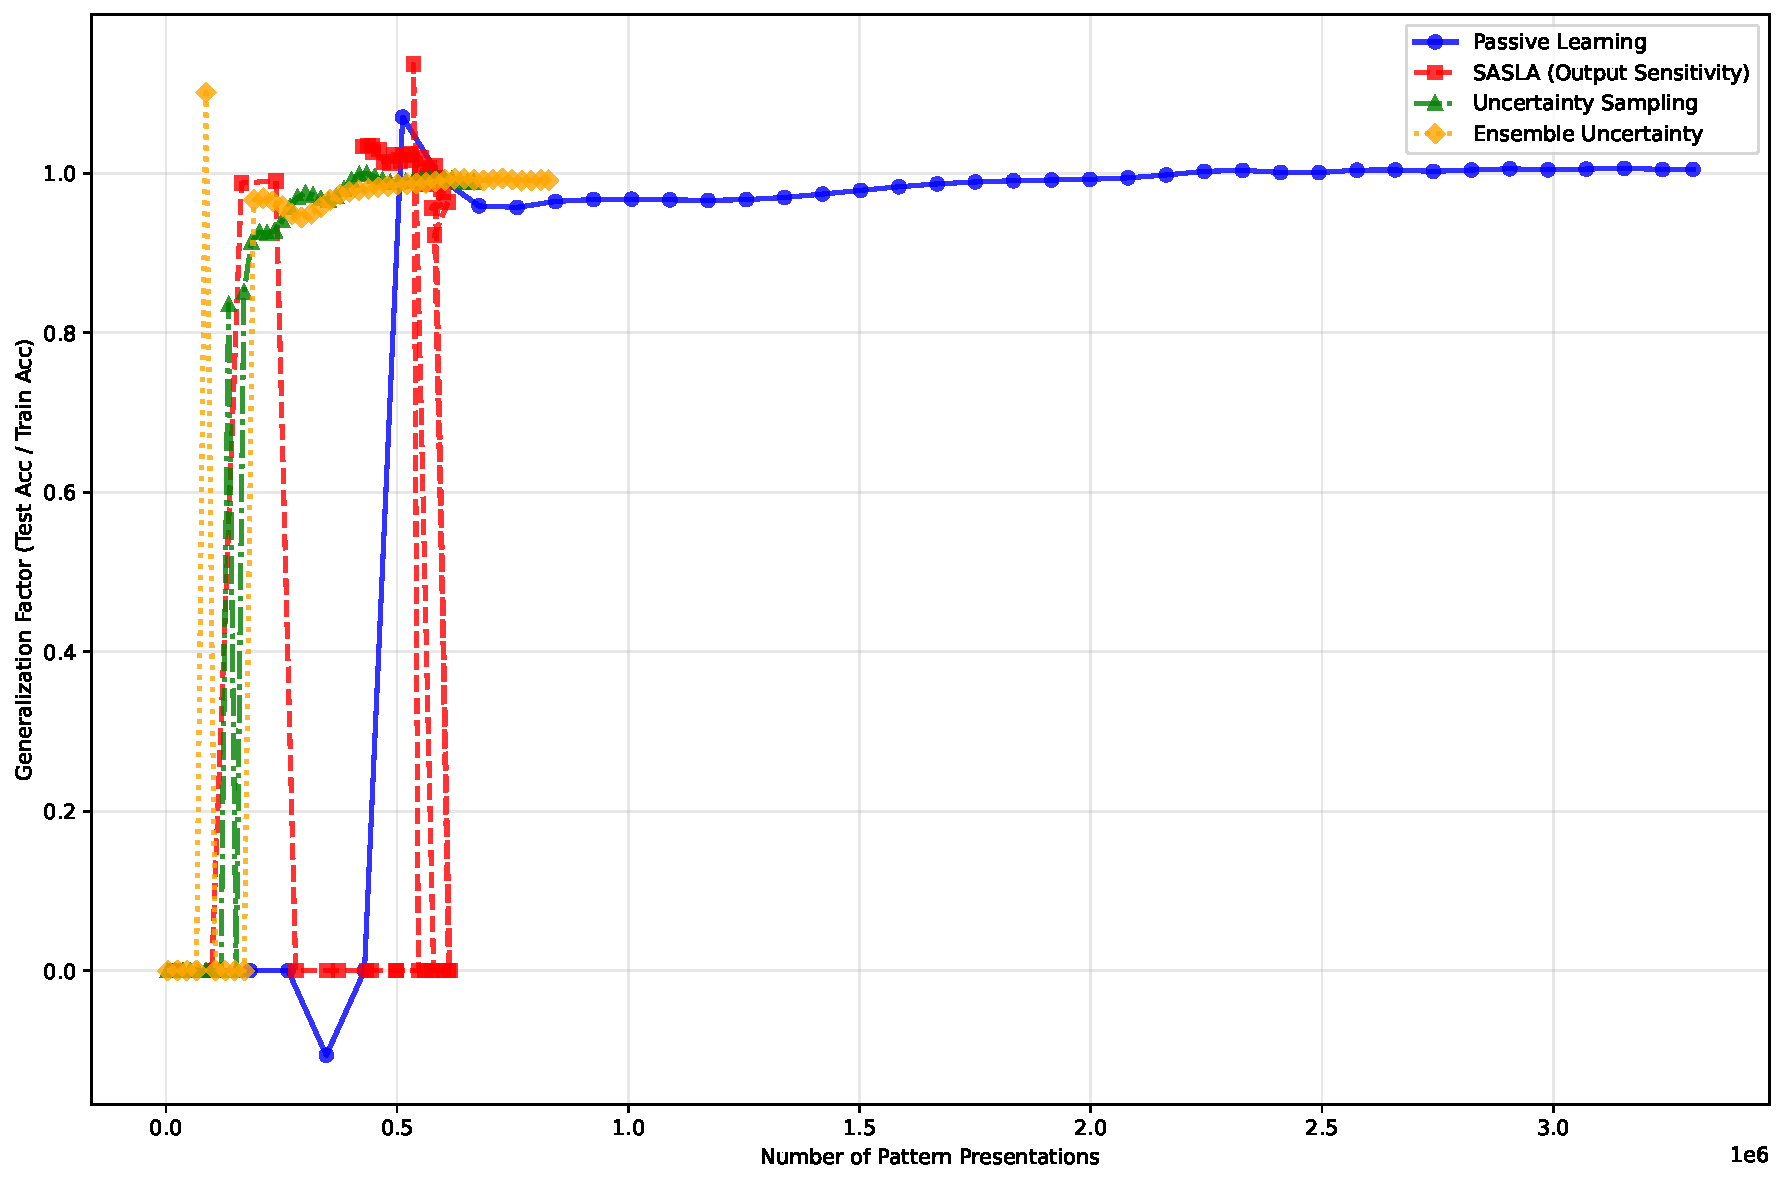
\includegraphics[width=\linewidth]{../results/housing/generalization_factor_vs_presentations.pdf}
	\caption{Generalisation factor versus number of pattern presentations for the California housing dataset.}
	\label{fig:gf_housing}
\end{figure}

%\begin{figure}[!t]
%	\centering
%	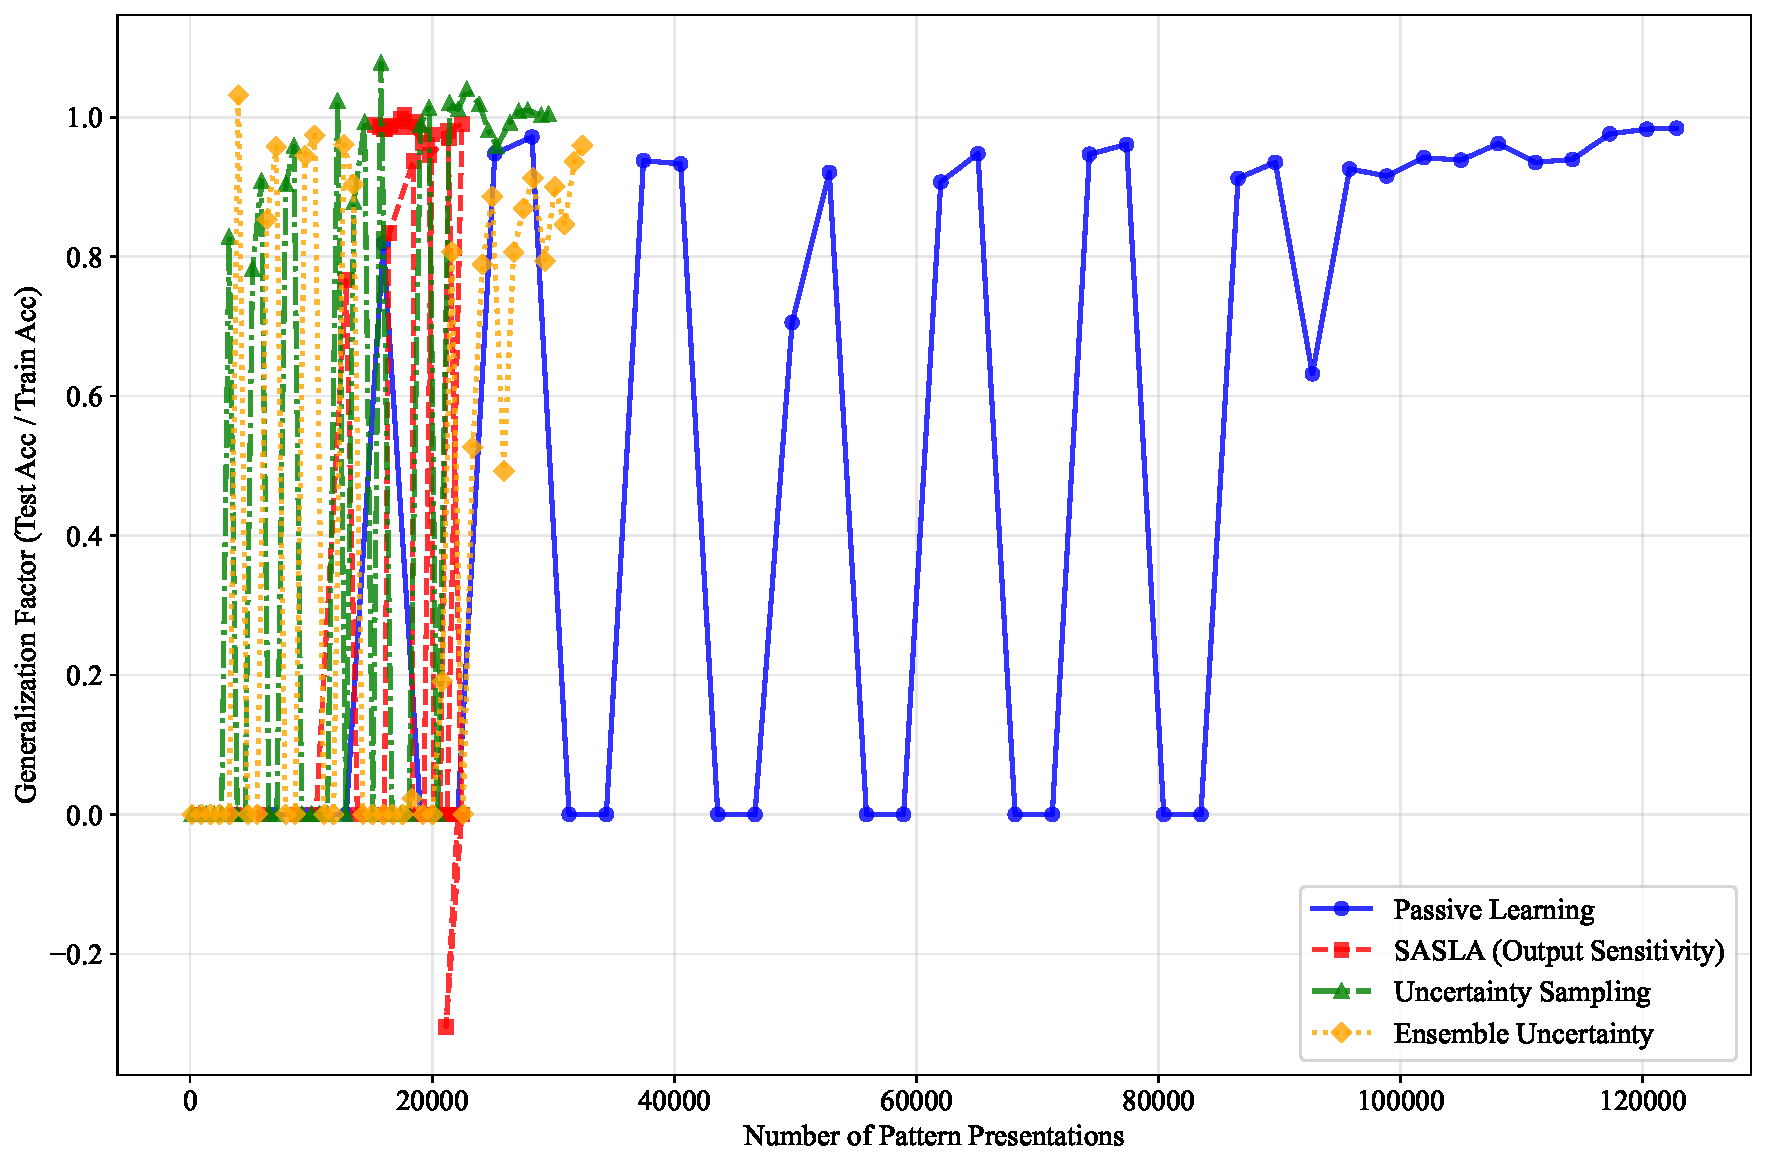
\includegraphics[width=\linewidth]{../results/energy/generalization_factor_vs_presentations.pdf}
%	\caption{Generalisation factor versus number of pattern presentations for the energy efficiency dataset.}
%	\label{fig:gf_energy}
%\end{figure}


\begin{figure}[!t]
	\centering
	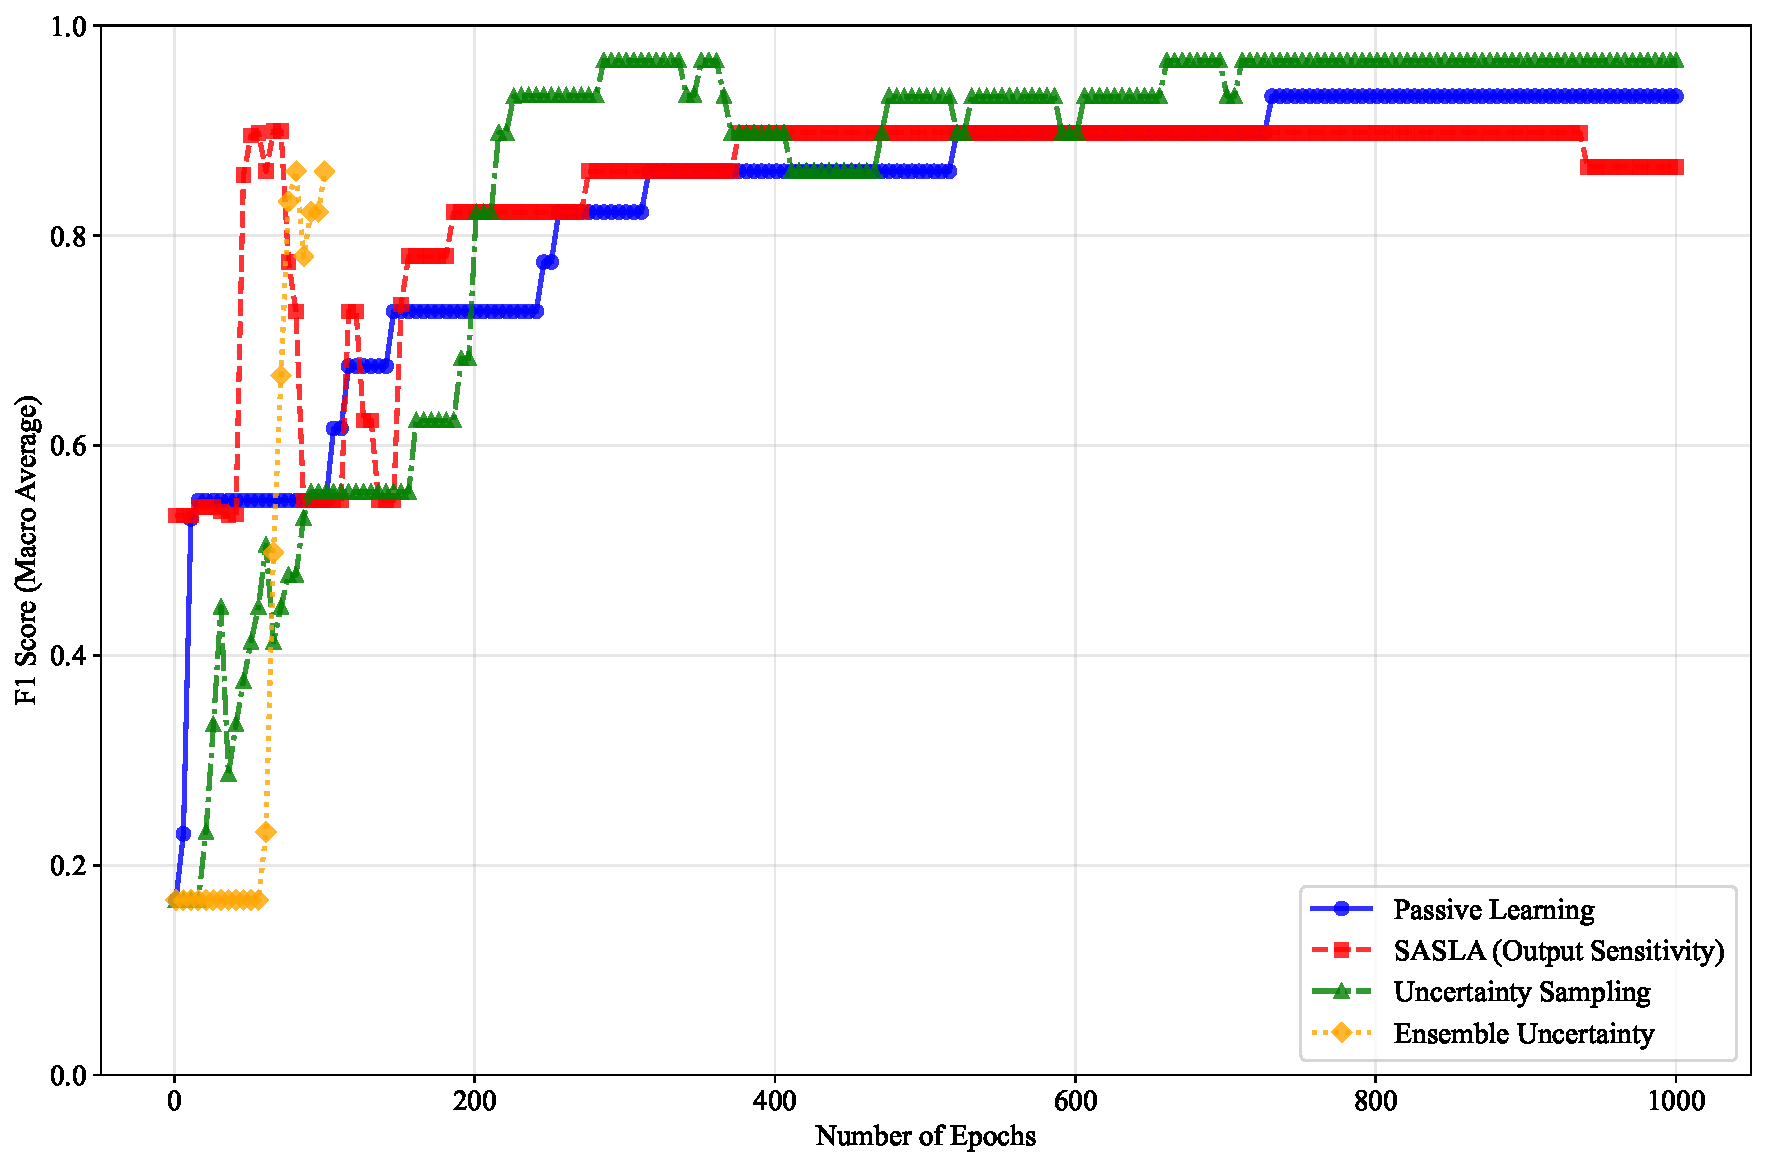
\includegraphics[width=\linewidth]{../results/iris/f1_score_vs_epochs.pdf}
	\caption{F1 score versus number of epochs for the iris dataset.}
	\label{fig:f1_iris}
\end{figure}

\begin{figure}[!t]
	\centering
	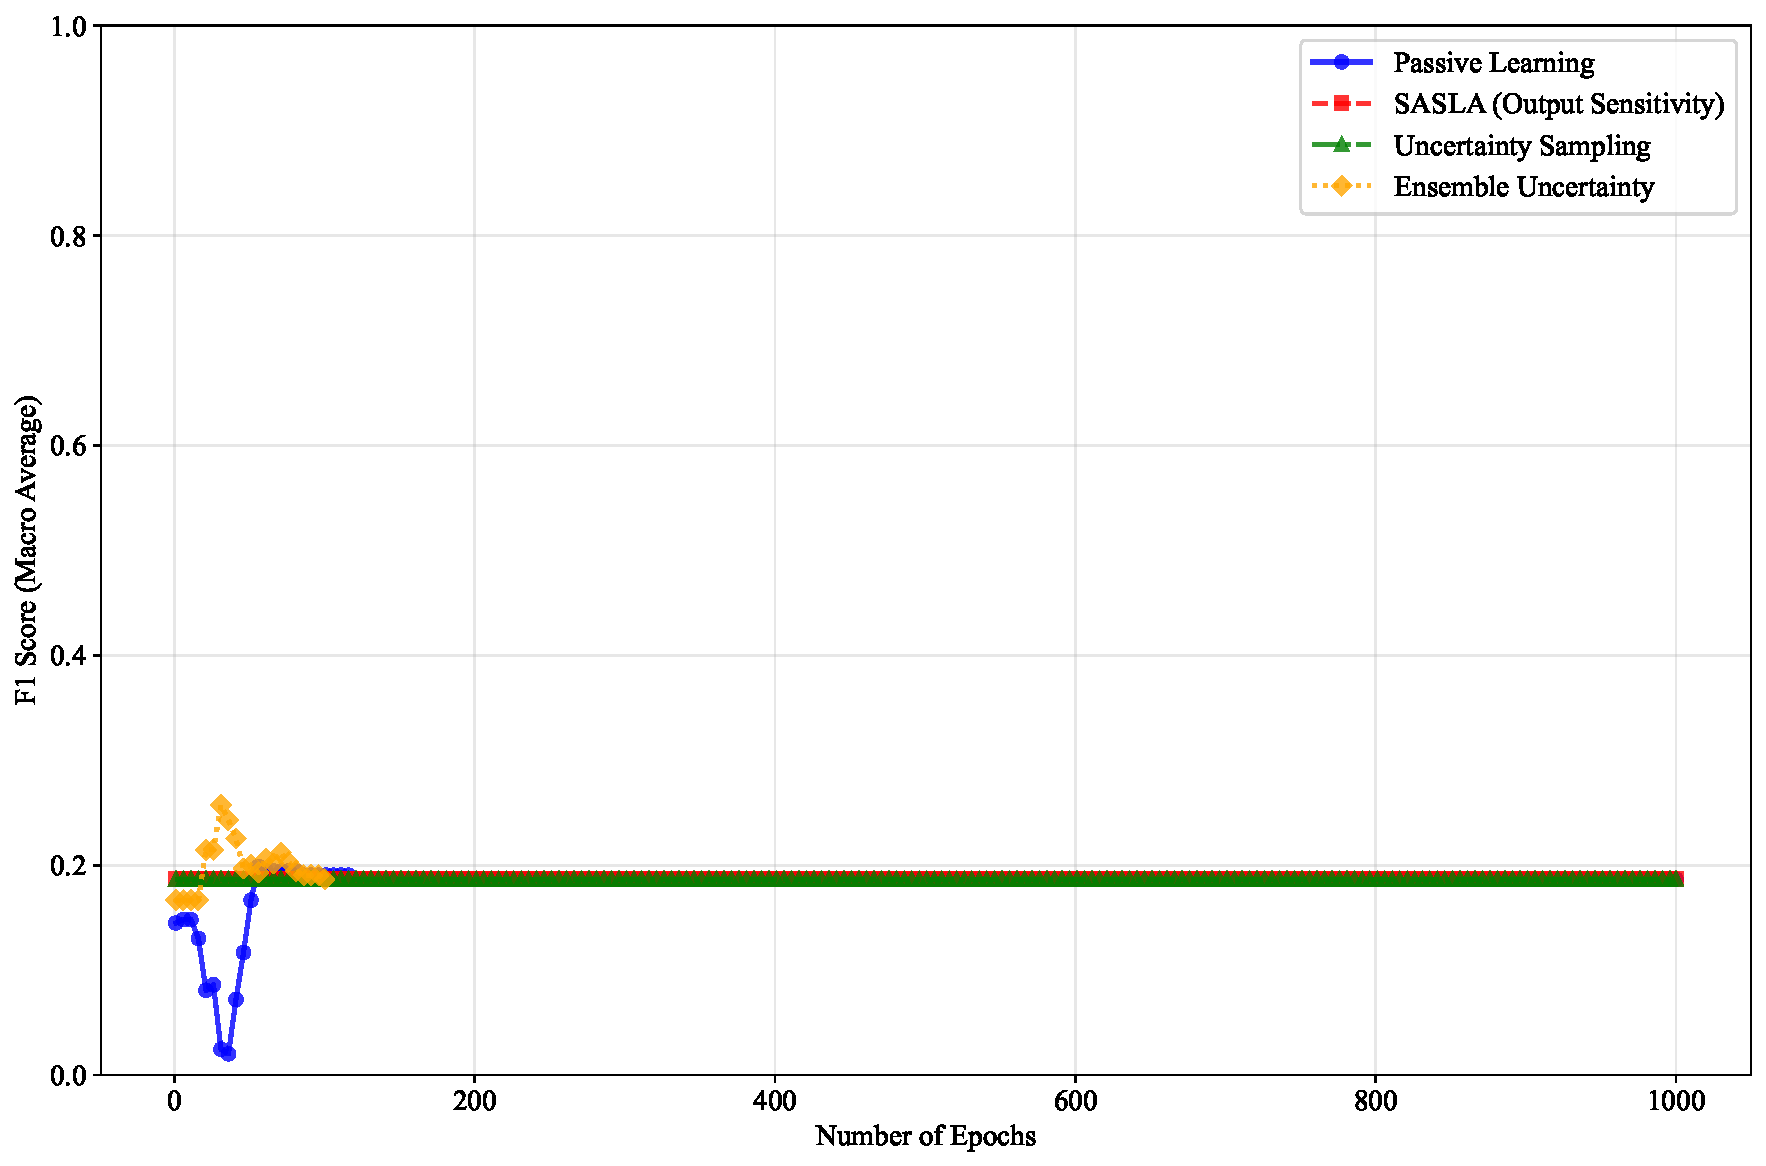
\includegraphics[width=\linewidth]{../results/wine/f1_score_vs_epochs.pdf}
	\caption{F1 score versus number of epochs for the wine dataset.}
	\label{fig:f1_wine}
\end{figure}

\begin{figure}[!t]
	\centering
	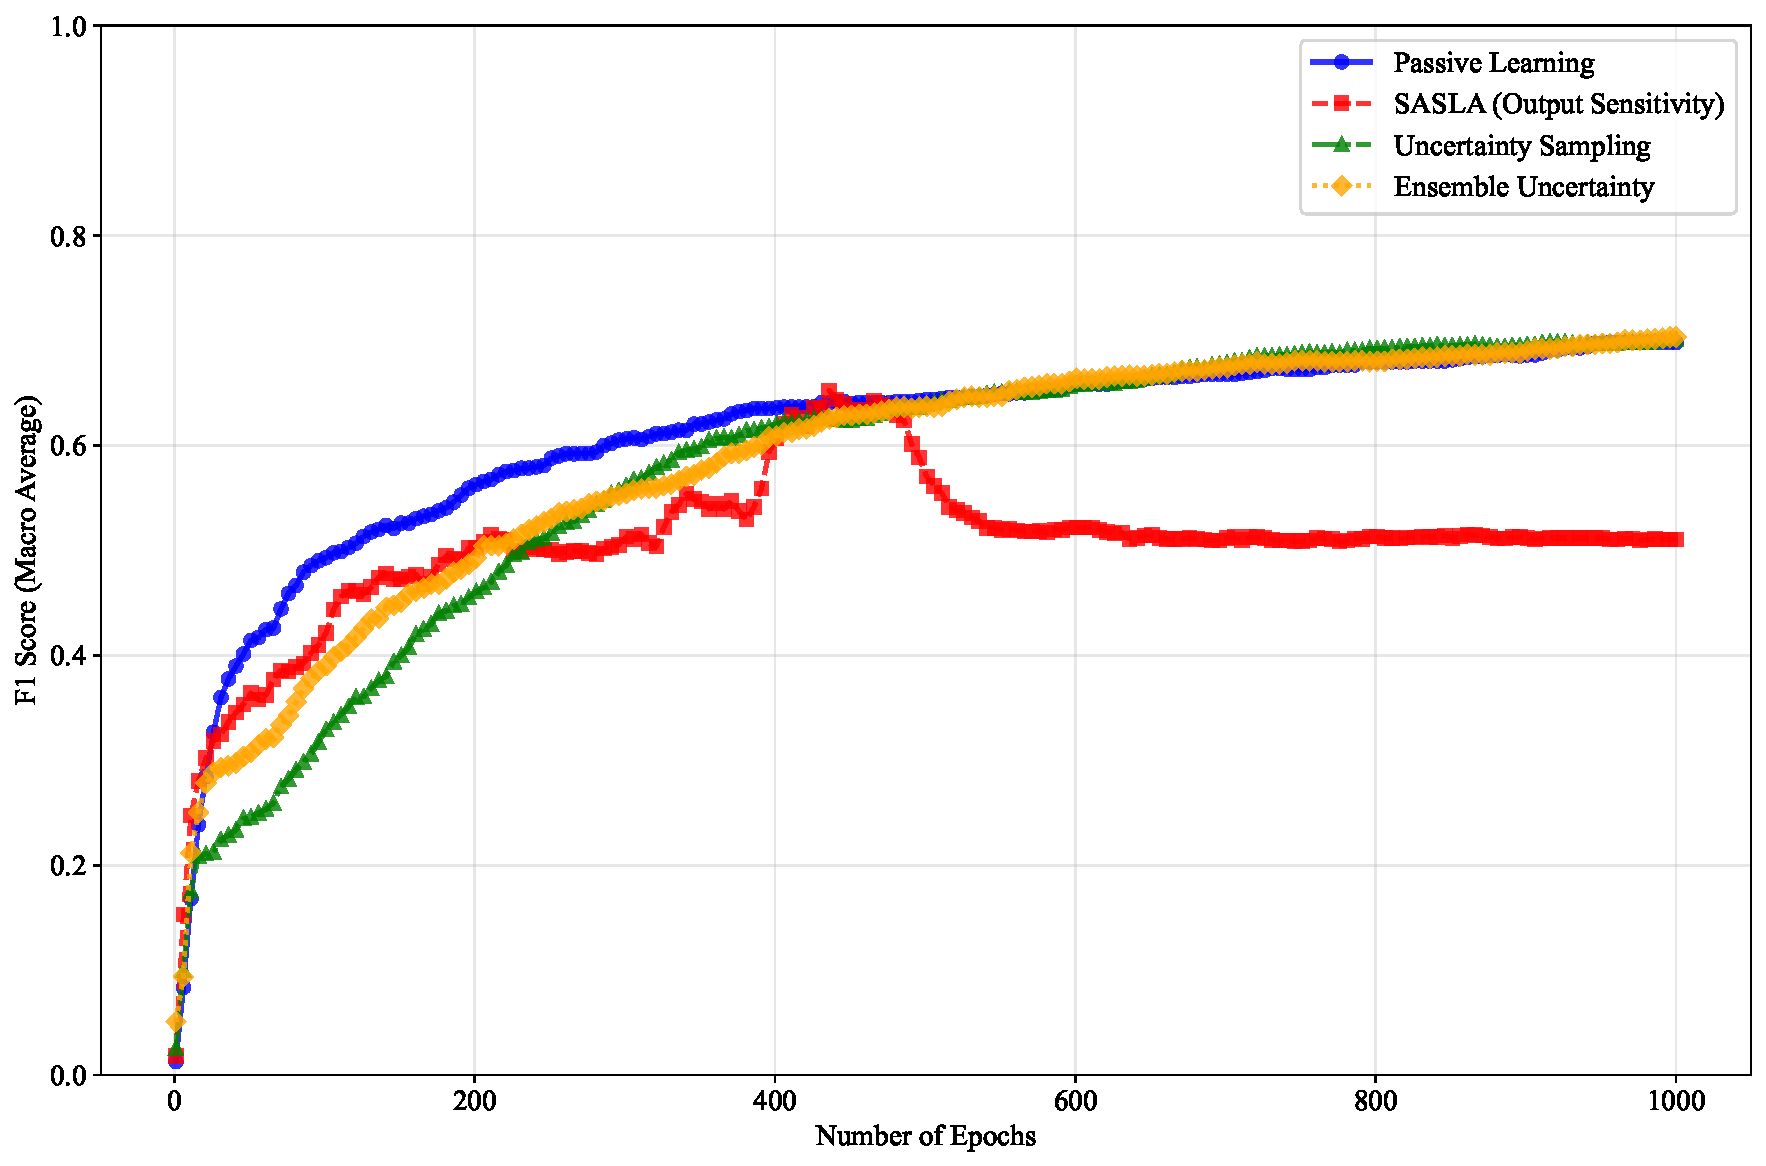
\includegraphics[width=\linewidth]{../results/fashion/f1_score_vs_epochs.pdf}
	\caption{F1 score versus number of epochs for the fashion-mnist dataset.}
	\label{fig:f1_fashion}
\end{figure}

\begin{figure}[!t]
	\centering
	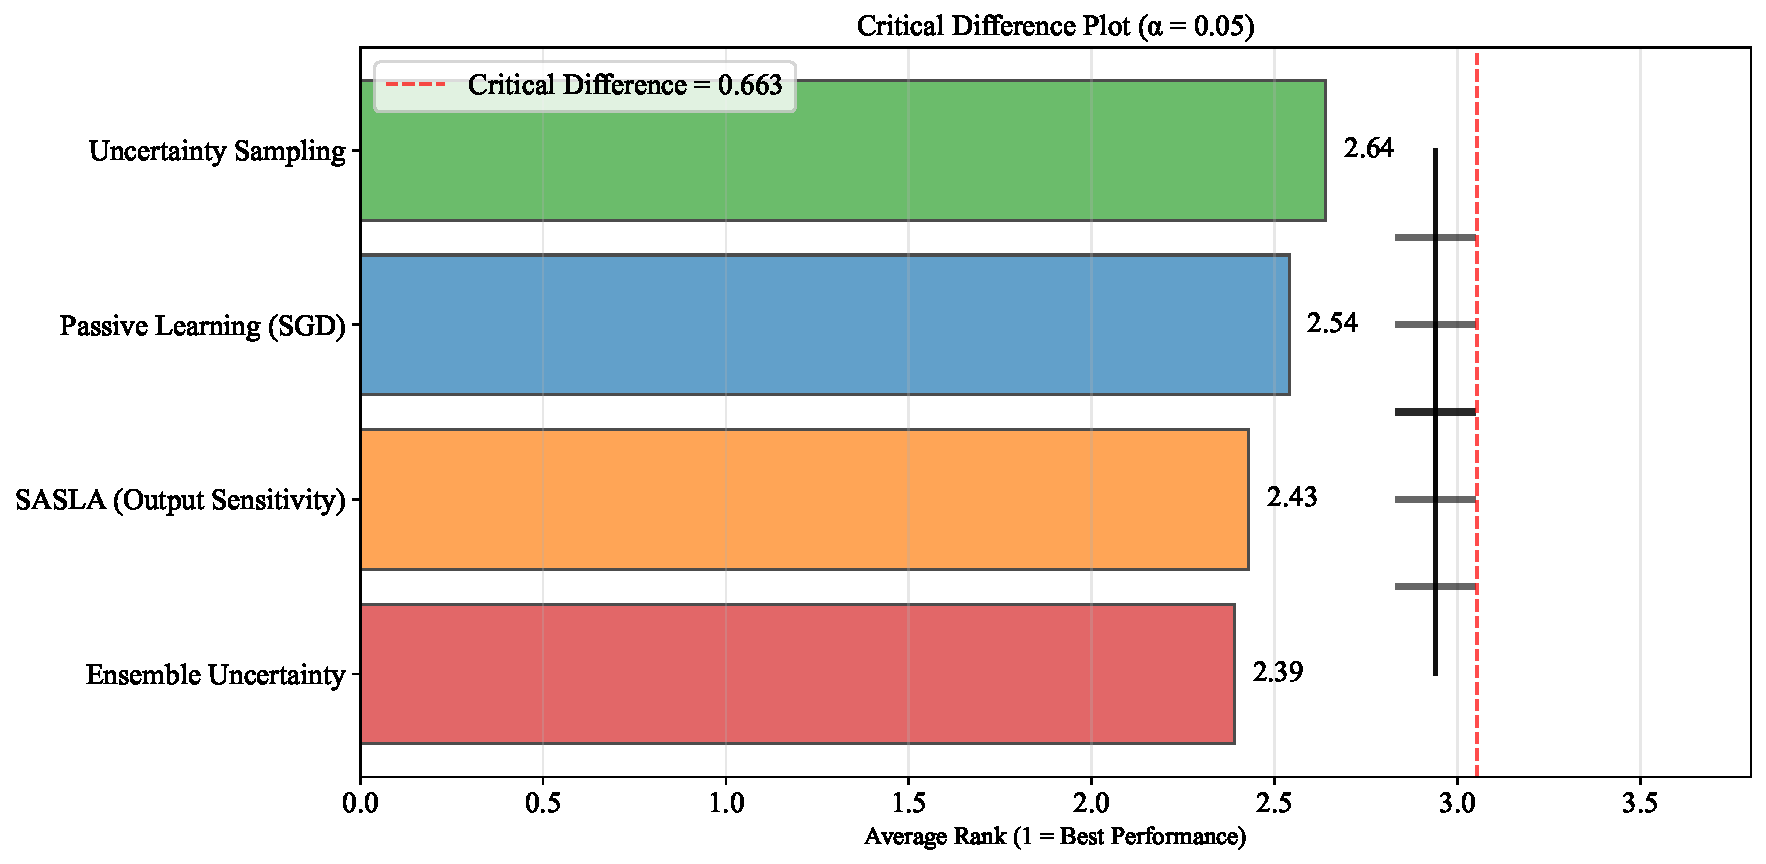
\includegraphics[width=\linewidth]{../results/iris/critical_difference_plot.pdf}
	\caption{Critical difference plot for the iris dataset.}
	\label{fig:cd_iris}
\end{figure}

%\begin{figure}[!t]
%	\centering
%	\includegraphics[width=\linewidth]{../results/wine/critical_difference_plot.pdf}
%	\caption{Critical difference plot for the wine dataset.}
%	\label{fig:cd_wine}
%\end{figure}

\begin{figure}[!t]
	\centering
	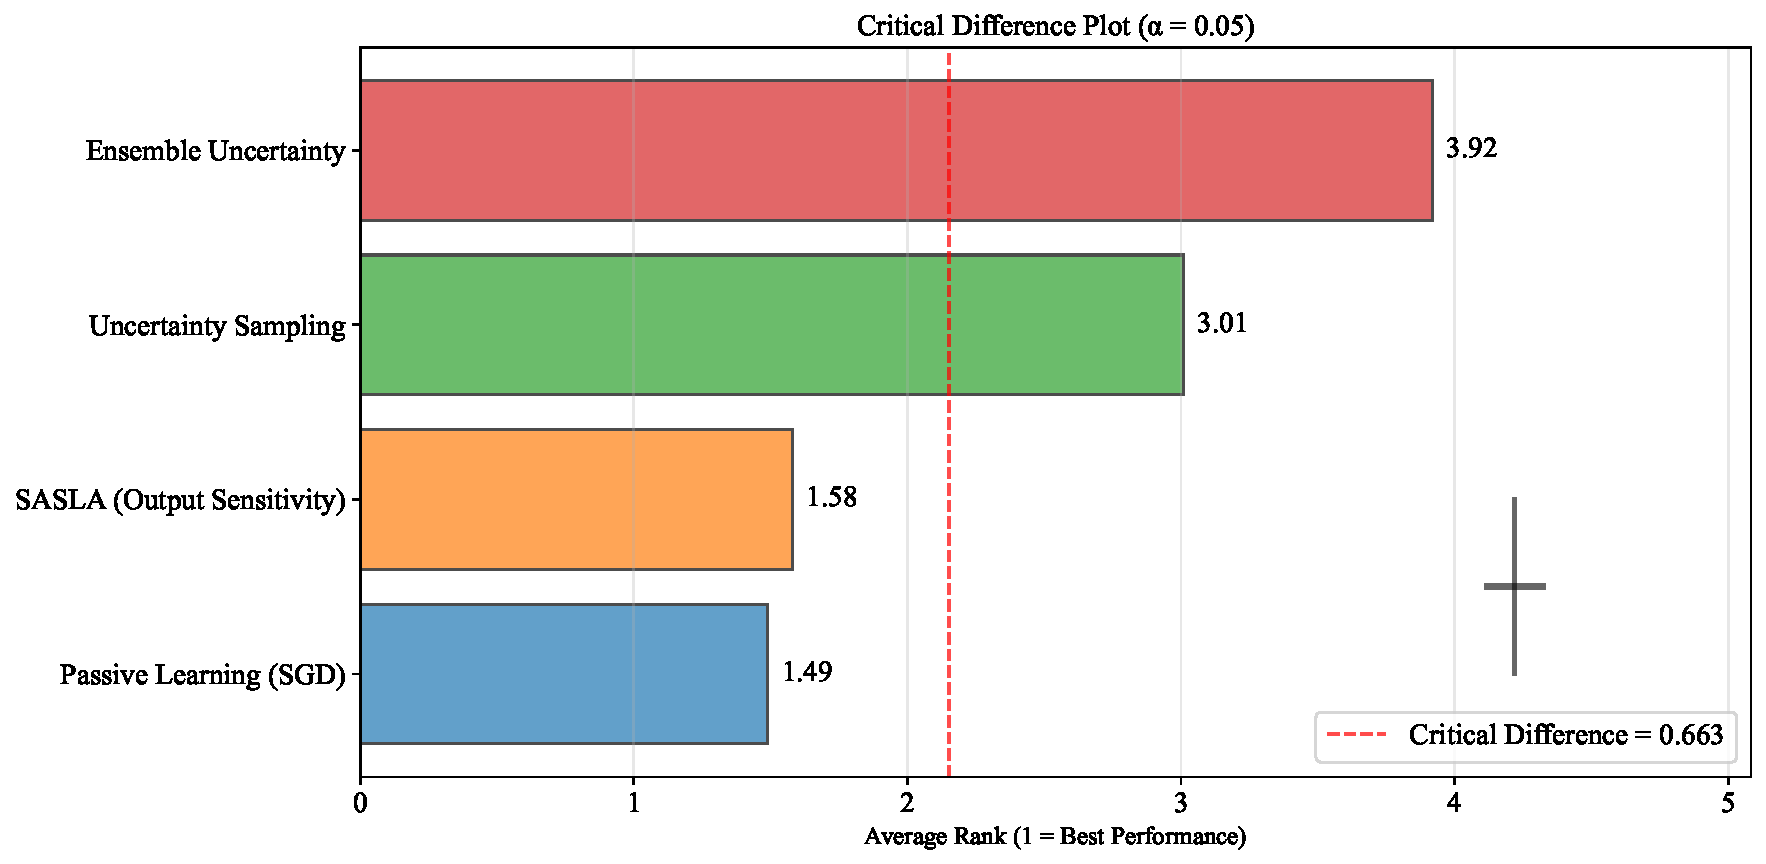
\includegraphics[width=\linewidth]{../results/fashion/critical_difference_plot.pdf}
	\caption{Critical difference plot for the fashion-mnist dataset.}
	\label{fig:cd_fashion}
\end{figure}

\begin{figure}[!t]
	\centering
	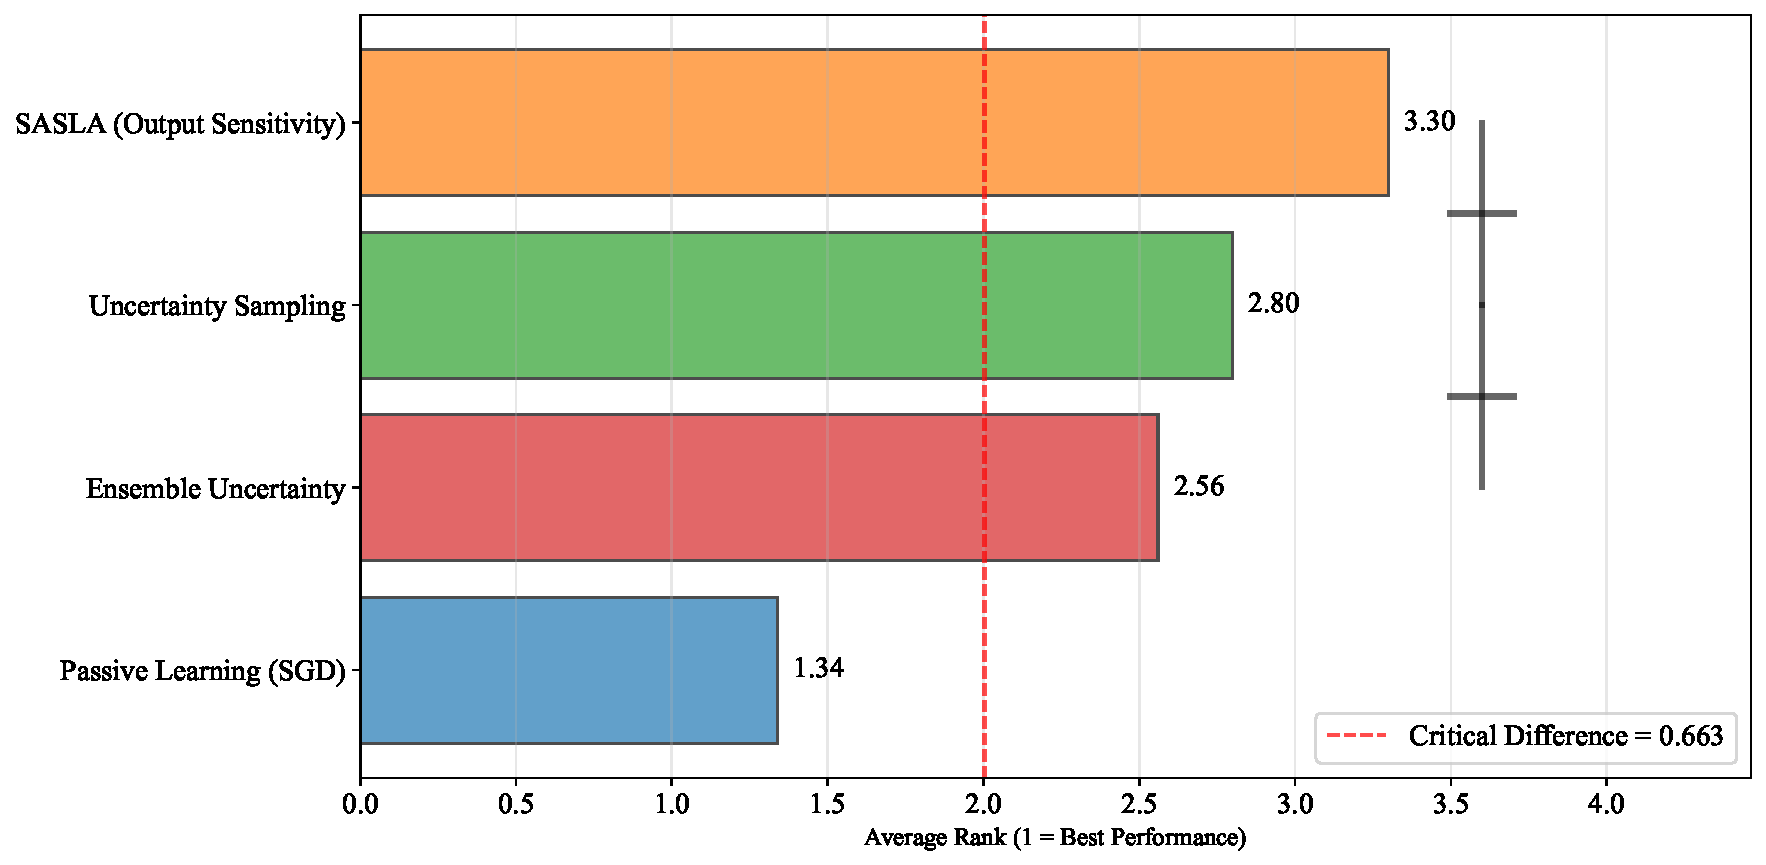
\includegraphics[width=\linewidth]{../results/synfunc/critical_difference_plot.pdf}
	\caption{Critical difference plot for the synthetic function dataset.}
	\label{fig:cd_synfunc}
\end{figure}

\begin{figure}[!t]
	\centering
	\includegraphics[width=\linewidth]{../results/housing/critical_difference_plot.pdf}
	\caption{Critical difference plot for the California Housing dataset.}
	\label{fig:cd_housing}
\end{figure}

\begin{figure}[!t]
	\centering
	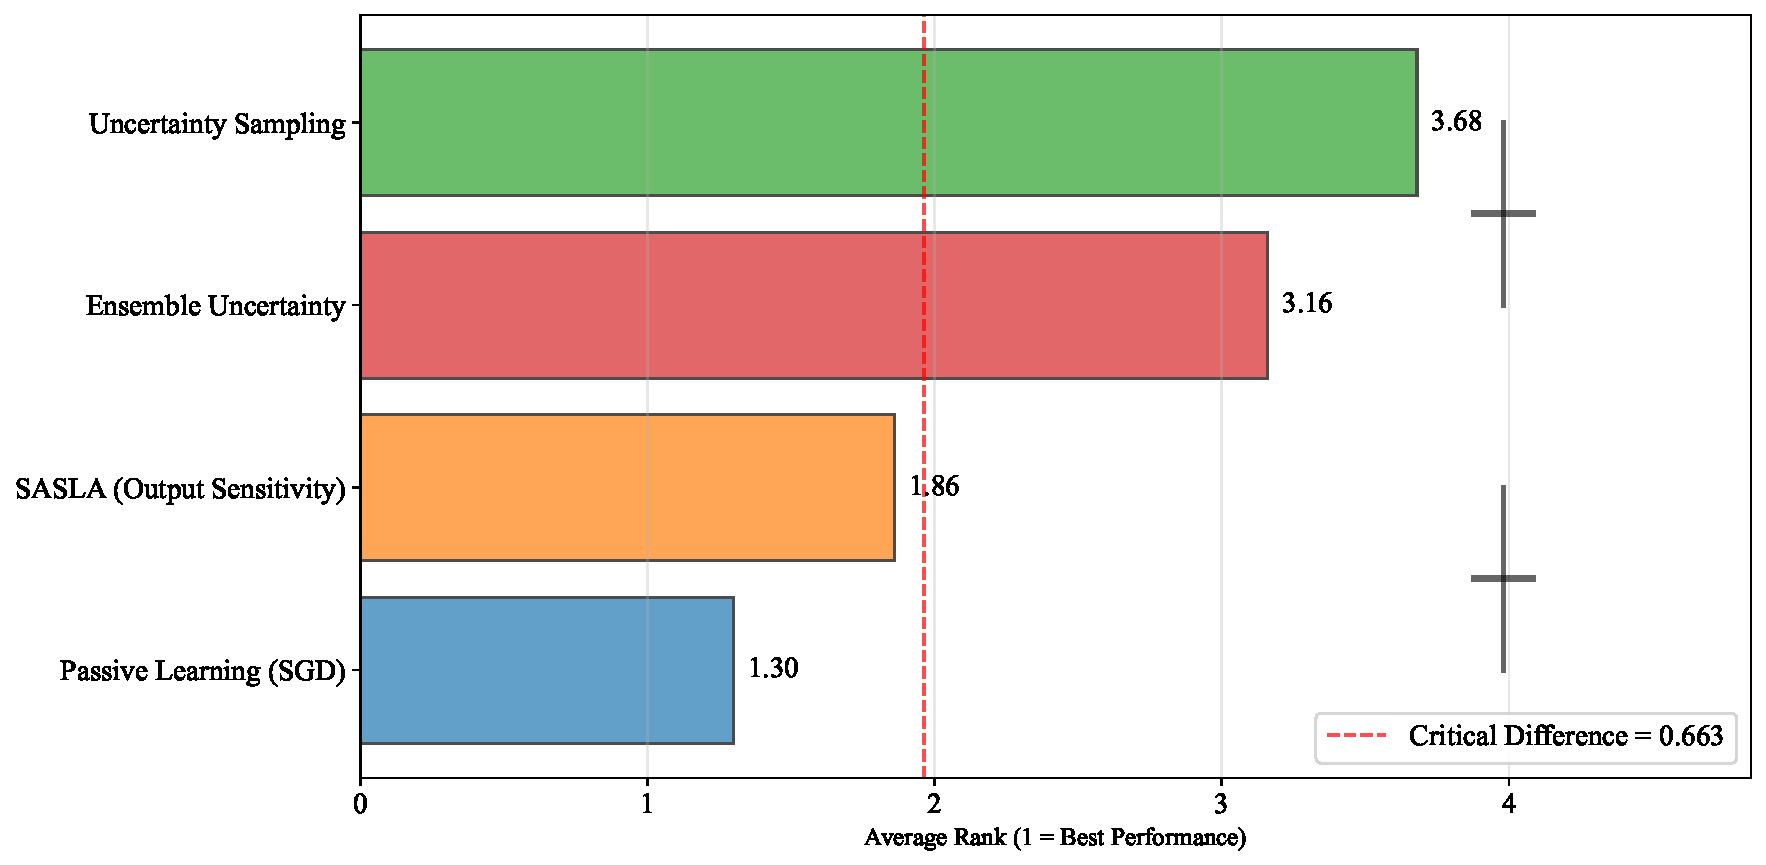
\includegraphics[width=\linewidth]{../results/energy/critical_difference_plot.pdf}
	\caption{Critical difference plot for the energy efficiency dataset.}
	\label{fig:cd_energy}
\end{figure}



\end{document}
